\documentclass[a4paper,12pt]{book}
%\usepackage[utf8]{inputenc}         %What is this?

%%%%%%%%%%%%%%%%%%%%%%%%%
%%% Document preamble %%%
%%%%%%%%%%%%%%%%%%%%%%%%%

\usepackage{appendix}
\usepackage[english]{babel}   %Spell-checker
%% extra symbols
\usepackage{amsmath}
\usepackage{amssymb}
\usepackage{wasysym}
%\usepackage{gensymb}    %Package not found ...
% hyperref
\usepackage[plainpages=false,pdfpagelabels=true,naturalnames=false,colorlinks=true,linkcolor=blue,citecolor=magenta,a4paper]{hyperref} %% online version
%\usepackage[plainpages=false,pdfpagelabels=true,naturalnames=false,colorlinks=false,linkcolor=blue,citecolor=magenta]{hyperref} %% print version 
% nice citations; hypernat needed to make natbib and hyperref interoperate
\usepackage[sort&compress,square,comma,numbers]{natbib}
\usepackage{hypernat}
% for figures
\usepackage{pstricks}
\usepackage{graphicx} 

\usepackage{caption}
\usepackage{subcaption}

%\usepackage{feynmf}    %Package not found
%\usepackage{axodraw} 

\usepackage{xspace}
\usepackage{color}
%\usepackage[center,tight]{subfigure}
\usepackage{eso-pic}
\usepackage{multirow}
\usepackage{epigraph}
% allow more text and floats per page
\renewcommand{\textfraction}{0.10}
\renewcommand{\topfraction}{0.90}
\setcounter{totalnumber}{5}

% change fonts: 
\usepackage[T1]{fontenc} % Needed? Makes feynmf crash...
\usepackage[utf8]{inputenc}

% latin modern
%\usepackage{lmodern}
% sans serif for normal text
%\renewcommand*\familydefault{\sfdefault}     %STIJN
% sans serif for math text
%\usepackage[lm]{sfmath}                      %STIJN
%\usepackage{helvet}
%% Choose one of the following (if not choosing the default, 
%% viz., Computer Modern, font family):
 %\usepackage{lmodern}
 %\usepackage{mathpazo}  %Can't write sigma
 %\usepackage{kpfonts} % CAVAKES
 %\usepackage{mathptmx}  %VUIL
 %\usepackage{times,mtpro2}
 %\usepackage{stix}
 %\usepackage{txfonts}   %VUIL
 %\usepackage{bookman}    %HEEL VUIL
 %\usepackage{newcent}   %VUIL
 %\usepackage{charter}    %OK, wiskundige symbolen slecht :(
 %\usepackage{chancery}   %VERKEERD!!
 %\usepackage{cmbright} % CAVAKES, min of meer
 %\usepackage{fourier} % NIET OK
 %\usepackage{euler} % NIET OK
 %\usepackage[adobe-utopia]{mathdesign}  %NIET OK
 % \usepackage[light,math,condensed]{anttor}  %ZEER RAAR
 % \usepackage{boisik} %Lelijk
 %\usepackage[bitstream-charter]{mathdesign}  %Voor mij ok, afgeprint zien
 %\usepackage{pxfonts}  %Precies onduidelijk om te lezen

% try to get dot working
% from http://www.maths.qmul.ac.uk/~rwb/latex.html
\DeclareSymbolFont{upright}       {OT1}{pnc}{m}{n}
\DeclareMathAccent{\dot}{\mathalpha}{upright}{"5F}  % single dot
\DeclareMathAccent{\ddot}{\mathalpha}{upright}{"7F} % double dot
\DeclareMathAccent{\bar}{\mathalpha}{upright}{"16}  % bar

% adjust page width (needs to be done before fancy headers)
\addtolength{\textwidth}{18mm}
% fancy page headers
\usepackage{fancyhdr}
\pagestyle{fancy}
\renewcommand{\chaptermark}[1]{\markboth{\MakeUppercase{\chaptername}\ \thechapter:\ #1}{}}
\renewcommand{\sectionmark}[1]{}
\fancyhf{}
\fancyhead[LE,RO]{\begin{footnotesize}\thepage\end{footnotesize}}
\fancyhead[RE,LO]{\begin{small}\leftmark\end{small}}
\renewcommand{\headrulewidth}{0.4pt}
% adjust rest of page layout (needs to be done after fancy headers)
\addtolength{\headheight}{2.5pt} % bring header closer
\addtolength{\headsep}{-2.5pt}
\addtolength{\topmargin}{-10mm} % enlarge vertical space
\addtolength{\textheight}{25mm}
\addtolength{\oddsidemargin}{-8mm} % adjust odd&even margins for texwidth
\addtolength{\evensidemargin}{-10mm}
% Add rotating possibility in columns and such
\usepackage{rotating}
% Add table row/column spans, extra space
\usepackage{multirow,array}
% Add linenumbers
\usepackage{lineno}      %Package not found
%\linenumbers

% my definitions
%My definitions!!
\newcommand{\ttbar}{t\bar{t}}
\newcommand{\gR}{g_{R}}
\newcommand{\csTh}{\cos \theta^{*}}
\newcommand{\DO}{D\O}
\newcommand{\DZ}{D$\varnothing$~}
\newcommand{\LWtb}{\mathcal{L}_{Wtb}}

% Units
\newcommand{\unit}[1]{\, \mathrm{#1}}	% units: roman + small space before
\newcommand{\eV}{\unit{eV}}		% electronvolt
\newcommand{\MeV}{\unit{MeV}}		% mega-electronvolt
\newcommand{\GeV}{\unit{GeV}}		% giga-electronvolt
\newcommand{\TeV}{\unit{TeV}}		% tera-electronvolt
\newcommand{\pbinv}{\pb^{-1}}		% 1/picobarn
\newcommand{\Hz}{\unit{Hz}}		% hertz
\newcommand{\MHz}{\unit{MHz}}		% megahertz
\newcommand{\km}{\unit{km}}             % kilometer
\newcommand{\cm}{\unit{cm}}             % centimeter
\newcommand{\mm}{\unit{mm}}             % millimeter
\newcommand{\m}{\unit{m}}               % meter
\newcommand{\s}{\unit{s}}               % second
\newcommand{\ns}{\unit{ns}}             % nanosecond
\newcommand{\K}{\unit{K}}               % Kelvin
\newcommand{\T}{\unit{T}}               % Tesla
\newcommand{\Tesla}{\unit{Tesla}}
\newcommand{\pbI}{\unit{pb}^{-1}}
\newcommand{\fbI}{\unit{fb}^{-1}}
\newcommand{\mum}{\mu\unit{m}}

%Kinematic information
\newcommand{\pT}{p_{\rm T}}
\newcommand{\ET}{E_{\rm T}}
\newcommand{\px}{p_{\rm x}}
\newcommand{\py}{p_{\rm y}}
\newcommand{\pz}{p_{\rm z}}
\newcommand{\kT}{k_{\rm T}}

% Program names
\newcommand{\FORTRAN}{\texttt{FORTRAN}}
\newcommand{\Pythia}{\texttt{PYTHIA}}
\newcommand{\FASTSIM}{\texttt{FASTSIM}}
\newcommand{\MGME}{\texttt{MadGraph/MadEvent}}
\newcommand{\Herwig}{\texttt{HERWIG}}
\newcommand{\Geant}{\texttt{GEANT4}}
\newcommand{\Madgraph}{\texttt{MADGRAPH}}
\newcommand{\Madweight}{\texttt{MADWEIGHT}}
\newcommand{\Powheg}{\texttt{PowHeg}}
\newcommand{\MCNLO}{\texttt{MC@NLO}}

%QCD coupling
\newcommand{\alpS}{\alpha_{S}}

%Missing transverse energy
\def\eslash{\ensuremath{{\hbox{$E$\kern-0.6em\lower-.05ex\hbox{/}\kern0.10em}}}}
\def\vecmet{\mbox{$\vec{\eslash}_T$}\xspace} %missing ET vector
\def\met{\mbox{$\eslash_T$}\xspace}

%Indent when using special paragraph listing
\newcommand{\indPar}{\hspace{3.5ex}}

%-------------------------------------------------------------------------------------------------

% % Units
% \newcommand{\unit}[1]{\, \mathrm{#1}}	% units: roman + small space before
% \newcommand{\eV}{\unit{eV}}		% electronvolt
% \newcommand{\MeV}{\unit{MeV}}		% mega-electronvolt
% \newcommand{\GeV}{\unit{GeV}}		% giga-electronvolt
% \newcommand{\TeV}{\unit{TeV}}		% tera-electronvolt
% \newcommand{\mb}{\unit{mb}}		% millibarn
% \newcommand{\mub}{\unit{\mu b}}		% microbarn
% \newcommand{\nb}{\unit{nb}}		% nanobarn
% \newcommand{\pb}{\unit{pb}}		% picobarn
% \newcommand{\pbinv}{\pb^{-1}}		% 1/picobarn
% \newcommand{\fb}{\unit{fb}}		% femtobarn
% \newcommand{\fbinv}{\fb^{-1}}		% 1/femtobarn
% \newcommand{\km}{\unit{km}}		% kilometer
% \newcommand{\m}{\unit{m}}		% meter
% \newcommand{\cm}{\unit{cm}}		% centimeter
% \newcommand{\mm}{\unit{mm}}		% millimeter
% \newcommand{\mum}{\unit{\mu m}}		% micrometer
% \newcommand{\fm}{\unit{fm}}		% femtometer
% \newcommand{\second}{\unit{s}}		% second
% \newcommand{\mus}{\unit{\mu s}}		% nanosecond
% \newcommand{\ns}{\unit{ns}}		% nanosecond
% \newcommand{\ps}{\unit{ps}}		% picosecond
% \newcommand{\Hz}{\unit{Hz}}		% hertz
% \newcommand{\MHz}{\unit{MHz}}		% megahertz
% \newcommand{\rad}{\unit{rad}}           % rad
% % Particles
% \newcommand{\pr}{$p$}		% proton
% \newcommand{\uq}{$u$}		% up quark
% \newcommand{\dq}{$d$}		% down quark
% \newcommand{\sq}{$s$}		% strange quark
% \newcommand{\cq}{$c$}		% charm quark
% \newcommand{\bq}{$b$}		% bottom quark
% \newcommand{\tq}{$t$}		% top quark
% \newcommand{\qq}{$q$}		% general quark q
% \newcommand{\Qq}{$Q$}		% heavy quark Q
% \newcommand{\gl}{$g$}		% gluon
% \newcommand{\uds}{$uds$}            % uds quarks
% \newcommand{\udsg}{$udsg$}          % udsg partons
% \newcommand{\jet}{$j$}		% jet in general
% \newcommand{\Z}{$Z$}		% Z boson
% \newcommand{\W}{$W$}		% W boson
% \newcommand{\Wpm}{\W$^{\pm}$}		% W+-
% \newcommand{\cH}{$H^{\pm}$}         % charged Higgs boson
% % Processes
% \newcommand{\ttbar}{\tq\bar{\tq}}
% \newcommand{\bbbar}{\bq\bar{\bq}}
% \newcommand{\ttbttj}{\tq\bar{\tq}\bq/\tq\bar{\tq}\jet}
% \newcommand{\ttbb}{\tq\bar{\tq}\bq\bar{\bq}}
% \newcommand{\ttjj}{\tq\bar{\tq}\jet\jet}
% \newcommand{\chhtotb}{\cH \to \tq\bq}
% \newcommand{\chhtotaunu}{\cH \to \tau\nu}
% % Special things
% \newcommand{\fixme}[1]{\textcolor{magenta}{{\bf FIX[}#1{\bf]}}}
% \newcommand{\todo}[1]{\textcolor{red}{{\bf TODO[}#1{\bf]}}}
% \newcommand{\ud}{\mathrm{d}}		% differential
% \newcommand{\Dcov}{\mathcal{D}}         % covariant derivative
% \newcommand{\LQCD}{\Lambda_\mathrm{QCD}}
% \newcommand{\tanbeta}{\tan \! \beta}
% \newcommand{\cotbeta}{\cot \! \beta}
% \newcommand{\BR}{{\rm BR}}		% branching ratio
% \newcommand{\LR}{\mathcal{L}}
% \newcommand{\DR}{\Delta R}
% \newcommand{\ET}{E_{\rm T}}
% \newcommand{\ETmiss}{E_{\rm T}^{\rm miss}}
% \newcommand{\pT}{p_{\rm T}}
% \newcommand{\pTmin}{p_{\rm T,min}}
% \newcommand{\kT}{k_{\rm T}}
% \newcommand{\mT}{m_{\rm T}}
% % Program names
% \newcommand{\FORTRAN}{\texttt{FORTRAN}}
% \newcommand{\VER}[1]{\texttt{#1}}
% \newcommand{\Pythia}{\texttt{PYTHIA}}
% \newcommand{\PYTHIAVER}[1]{\PYTHIA{} \VER{#1}}
% \newcommand{\HDECAY}{\texttt{HDECAY}}
% \newcommand{\HDECAYVER}[1]{\HDECAY{} \VER{#1}}
% \newcommand{\CMSJET}{\texttt{CMSJET}}
% \newcommand{\CMSJETVER}[1]{\CMSJET{} \VER{#1}}
% \newcommand{\FASTSIM}{\texttt{FASTSIM}}
% \newcommand{\MGME}{\texttt{MadGraph/MadEvent}}
% \newcommand{\Herwig}{\texttt{HERWIG}}
% \newcommand{\COMPHEP}{\texttt{CompHEP}}
% \newcommand{\COMPHEPVER}[1]{\COMPHEP{} \VER{#1}}
% \newcommand{\ALPGEN}{\texttt{ALPGEN}}
% \newcommand{\ALPGENVER}[1]{\ALPGEN{} \VER{#1}}
% \newcommand{\CMKIN}{\texttt{CMKIN}}
% \newcommand{\CMKINVER}[3]{\CMKIN{}\VER{\_#1\_#2\_#3}}
% \newcommand{\CMSIM}{\texttt{CMSIM}}
% \newcommand{\CMSIMVER}[1]{\CMSIM{}\VER{#1}}
% \newcommand{\COBRA}{\texttt{COBRA}}
% \newcommand{\OSCAR}{\texttt{OSCAR}}
% \newcommand{\OSCARVER}[3]{\OSCAR{}\VER{\_#1\_#2\_#3}}
% \newcommand{\ORCA}{\texttt{ORCA}}
% \newcommand{\ORCAVER}[3]{\ORCA{}\VER{\_#1\_#2\_#3}}
% \newcommand{\FAMOS}{\texttt{FAMOS}}
% \newcommand{\FAMOSVER}[3]{\FAMOS{}\VER{\_#1\_#2\_#3}}
% \newcommand{\GEANT}{\texttt{GEANT}}
% \newcommand{\GEANTVER}[1]{\GEANT{}\VER{#1}}
% \newcommand{\CRAB}{\texttt{CRAB}}
% \newcommand{\Madgraph}{\texttt{MADGRAPH}}
% \newcommand{\Madweight}{\texttt{MADWEIGHT}}
% % Colliders, Experiments,...
% \newcommand{\CERN}{CERN}
% \newcommand{\LEP}{{\sc LEP}}
% \newcommand{\Tevatron}{{\sc Tevatron}}
% \newcommand{\HERA}{{\sc HERA}}
% \newcommand{\DESY}{{\sc DESY}}
% \newcommand{\Delphi}{DELPHI}
% \newcommand{\Babar}{{\sc BaBar}}
% \newcommand{\Belle}{{\sc Belle}}
% \newcommand{\TOTEM}{{\sc Totem}}
% \newcommand{\ATLAS}{ATLAS}
% \newcommand{\ALICE}{ALICE}
% \newcommand{\LHCB}{LHCb}
% \newcommand{\LHCF}{LHCf}
% \newcommand{\CDF}{CDF}
% \newcommand{\DO}{D\O}
% %CHAPTER3
% \newcommand{\alpS}{\alpha_{S}}

% Random stuff
\newenvironment{myindentpar}%
{\begin{list}{}%
        {\setlength{\leftmargin}{0.5cm}}%
        \item[]%
}
{\end{list}}

\def\eslash{\ensuremath{{\hbox{$E$\kern-0.6em\lower-.05ex\hbox{/}\kern0.10em}}}}
\def\vecmet{\mbox{$\vec{\eslash}_T$}\xspace} %missing ET vector
\def\met{\mbox{$\eslash_T$}\xspace}


\usepackage{titlesec}
\titleformat{\chapter}[display]
  {\bfseries\huge}
%  {\filleft\Large\chaptertitlename~\thechapter}
  {\hrulefill ~\Large\chaptertitlename~\thechapter ~\hrulefill}
%  {3ex}
  {0.3ex}
%  {\titlerule\vspace{1.5ex}\filright}
  {\filcenter}
  [\vspace{0.5ex}\titlerule]

%\makeatletter
%\def\thickhrulefill{\leavevmode \leaders \hrule height 1.2ex \hfill \kern \z@}
%\def\@makechapterhead#1{
%  \vspace*{10\p@}%
%  {\parindent \z@ \centering \reset@font
%        \thickhrulefill\quad 
%        \scshape\bfseries\textit{\@chapapp{}  \thechapter}  
%        \quad \thickhrulefill
%        \par\nobreak
%        \vspace*{10\p@}%
%        \interlinepenalty\@M
%        \hrule
%        \vspace*{10\p@}%
%        \Huge \bfseries #1 \par\nobreak
%        \par
%        \vspace*{10\p@}%
%        \hrule
%        \vskip 100\p@
%  }}

% my hyphenations
%\hyphenation{si-mu-la-ted stu-died middle-ware re-nor-ma-li-za-tion}

%%%%%%%%%%%%%%%%%%%%%%%%%%%
%%% The document itself %%%
%%%%%%%%%%%%%%%%%%%%%%%%%%%

\begin{document}
%\begin{linenumbers}

% \frontmatter     %Commented temporarily during writing to have the pagenumbers matching with the counter

% the titlepage
%\cleardoublepage
%
%  Titlepage
%
\thispagestyle{empty}

%\AddToShipoutPicture{
%  \AtPageCenter{
%    \begin{minipage}{3cm}
%      \vspace*{-18cm}
%      \hspace{-1.5cm}
\includegraphics[width=3cm,height=3cm]{FrontMatter/vublogo}%
%      \hspace{-3cm}\psframe[linecolor=white,fillstyle=crosshatch,hatchwidth=.05pt,hatchsep=1pt,hatchcolor=white](0,0)(3,3)
%    \end{minipage}
%  }
%}

\vspace*{-5mm}
\begin{minipage}{\textwidth}
  \begin{center}
%    \vspace{-3mm}\rule{\textwidth}{1pt}
    \begin{Large}
      Vrije Universiteit Brussel\\[6mm]
    \end{Large}
    
\includegraphics[width=0.4 \textwidth]{FrontMatter/vublogo}\\[6mm]
    \begin{large}
      Faculteit Wetenschappen en Bio-ingenieurswetenschappen\\
      Vakgroep Fysica\\
    \end{large}
  \end{center}
\end{minipage}

\vspace{1.5cm}
\begin{minipage}{\textwidth}
  \begin{flushleft}
%    \vspace{-5cm}\rule{1mm}{5cm}\rule{13cm}{1mm}
    \rule{\textwidth}{1mm}
    %\vspace{-0.1cm}
  \end{flushleft}
  \begin{center}
    \begin{bfseries}
      \begin{sffamily}
        \begin{Huge}%
          Measuring the anomalous couplings \\ \vspace{0.2cm}
          in the Wtb vertex using the Matrix \\ \vspace{0.4cm}
          Element Method at the LHC
        \end{Huge}
      \end{sffamily}
    \end{bfseries}
  \end{center}
%  \vspace{.5mm}
  \begin{flushright}
%    \rule[4.9cm]{13cm}{1mm}\rule{1mm}{5cm}\vspace{-5cm}
    \rule{\textwidth}{1mm}
  \end{flushright}
\end{minipage}

\vspace{1.5cm}
\begin{minipage}{\textwidth}
  \begin{center}
    \begin{bfseries}
      \begin{sffamily}
        \begin{LARGE}
          Annik Olbrechts\\
        \end{LARGE}
      \end{sffamily}
    \end{bfseries}
  \end{center}
\end{minipage}

\vspace{1.5cm}
\begin{minipage}{\textwidth}
  \begin{center}
    \begin{large}
      Promotor:  Prof. Dr. Jorgen D'Hondt\\[5mm]
      Proefschrift ingediend met het oog op het behalen van\\
      de academische graad Doctor in de Wetenschappen\\[10mm]
      %Month 2015
      Version: \today
    \end{large}
  \end{center}
\end{minipage}

%\vspace{-25cm}
%\begin{minipage}{\textwidth}
%    \begin{large}
%      \textcolor{magenta}{Preliminary --- Compiled on \today{}}
%    \end{large}
%\end{minipage}


\newpage
\thispagestyle{empty}

%\ClearShipoutPicture{}


%\vspace*{\stretch{1}}

\begin{large}

\begin{center}
\begin{minipage}{15cm}
Doctoral examination commission:\\[2mm]
%Prof. Dr. J. D'Hondt (Vrije Universiteit Brussel)\\%[0.5mm]
%Prof. Dr. B. Craps (Vrije Universiteit Brussel)\\%[0.5mm]
%Prof. Dr. F. Blekman (Vrije Universiteit Brussel)\\%[0.5mm]
%Prof. Dr. F. Maltoni (Université Catholique de Louvain)\\%[0.5mm]
%Prof. Dr. N. Van Eijndhoven (Vrije Universiteit Brussel)\\%[0.5mm]
%Prof. Dr. P. Vanlaer (Université Libre de Bruxelles) \\%[0.5mm]
%(Prof.) Dr. P. Van Mulders (Vrije Universiteit Brussel)\\
%Prof. Dr. W. De Meuter (Vrije Universiteit Brussel)\\[1cm]


%This thesis is realised with the financial support of IWT-Vlaanderen.\\[3cm]
%Cover illustration: Different visualisations of the reconstructed particles in the CMS detector originating from the decay of a semi-muonic $\ttbar$ event at a center of mass energy of 10\,TeV.\\[0.5mm]
%Print: Silhouet, Maldegem\\[0.5cm]
\copyright \, 2015 Annik Olbrechts\\[0.5cm]
%2010 Uitgeverij ASP (Academic and Scientific Publishers nv)\\%[0.5mm]
%Ravensteingalerij 28\\%[0.5mm]
%B-1000 Brussels\\%[0.5mm]
%Tel. + 32 (0)2 289 26 50\\%[0.5mm]
%Fax + 32 (0)2 289 26 59\\%[0.5mm]
%E-mail: info\@aspeditions.be\\%[0.5mm]
%www.aspeditions.be\\[0.5cm]
%ISBN 978 90 5487 761 5\\%[0.5mm]
%NUR 924\\%[0.5mm]
%Legal Deposit D/2010/11.161/085\\[1cm]
All rights reserved. No parts of this book may be reproduced or transmitted in any form or by
any means, electronic, mechanical, photocopying, recording, or otherwise, without the prior
written permission of the author.

\end{minipage}
\end{center}

\end{large}
%\vspace*{\stretch{1}}

%\newpage
%\thispagestyle{empty}


% the table of contents
\cleardoublepage
\phantomsection
%\addcontentsline{toc}{chapter}{Contents}
\tableofcontents

%\mainmatter        %Commented temporarily during writing to have the pagenumbers matching with the counter

% the introduction
\cleardoublepage
\phantomsection
%\addcontentsline{toc}{chapter}{Introduction}
%\chapter*{Introduction\markboth{\MakeUppercase{Introduction}}{}}


% the chapters
%%\dropchapter{0.4in}
\chapter{Anomalous couplings in the top quark sector} \label{chp::SM}
%\epigraphhead[70]{\epigraph{\textit{If I could remember the names of all these particles, I'd be a botanist.}}{Enrico Fermi}}
%\undodrop

%The ultimate goal of any particle physics is to \\
%Within experimental particle physics, the ultimate goal is to understand \\
Ever since the beginning of physics, and especially of particle physics, the ultimate goal is to progress and move forward in the understanding of the particles and their interactions observed around us. 
In order to achieve a new breakthrough on the level of elementary particle physics our current knowledge should continously be questioned and no detail, no matter how small, should be overlooked.
%** no stone should be left unturned **.
In this perspective the Standard Model of elementary particle physics should be seen as a first step towards a grand unification of all fundamental interactions which has met every test endured up to now.
%endured is ``tested to the limit'' time after time, but for the moment has met every test.
\\
\textit{Now shortly summarize what will be discussed in this chapter!}\\
\textbf{More focus ont he role of top in SM searches!}

\section{Standard Model of elementary particle physics}
The Standard Model of elementary particle physics (SM) is a theoretical framework designed in 1978 which contains three of the four fundamental interactions.

\subsection{Particle content}

The extensive search for elementary particles and the chain of discoveries during the 20$^{th}$ century continously altered the understanding of the fundamental theory describing them.
%It almost appears that every new particle discovery resulted in a complete destruction of the existing theory assumptions.
Every new discovery divided the physics community and often required the development of a completely new structure capable of describing the observations.
Hence the Standard Model, officially established in the early 1970s, actually consists of many ingenious contributions from many renown physicists~\cite{Griffiths}. 
For the last decades the general belief on elementary particles is conceived rather stable, especially since every new discovery validated the theory described by the Standard Model. % and summarized in Table~\ref{table::ElemParticles}.

The elementary particles have been subdivided based on their spin. Fermions, containing both leptons and quarks, have half-integer spin while bosons, also called force mediators, have integer spin. 
The collection of fermions can be stored into three separate generations, characterized by increasing mass, and is summarized in Table~\ref{table::ElemParticles}.  Each fermion $f$ has an antiparticle, which is defined to have the same mass but opposite electrical charge and is denoted as $\bar{f}$. The only exception is the antiparticle of the charged leptons $l^{-}$ which are represented as $l^{+}$.\\
Even though the Standard Model is only complete when all three generations are considered, the first one is the one which is relevant for describing all stable matter visible around us.
The up- and down-quarks can bond together to form protons and neutrons, with respective quark-content $uud$ and $udd$. Together with the electron this is sufficient to form atoms and hence build every known chemical element.
%The atom of each chemical element consists of a nucleus surrounded with electrons while the nucleus can be  
%The core of any nucleus atom consists of protons and neutrons, with quark-content $uud$ and $udd$, respectively, 
\setlength\extrarowheight{5pt}
\begin{table}[h!t]
 \centering
 \caption{Overview of the fermions in the Standard Model and their corresponding electrical charge.} \label{table::ElemParticles}
 \begin{tabular}{|c|cr|cc|cc|cc|c|}
  \hline
  \textbf{Generation} 		& \multicolumn{4}{c|}{\textbf{Quarks}} 				& \multicolumn{4}{c|}{\textbf{Leptons}} 				\\
  \hline
  1$^{st}$ 			& up 		& $u$ 		& down 		& $d$ 		& electron neutrino	& $\nu_{e}$ 	& electron	& $e^{-}$ 	\\
  \hline
  2$^{nd}$ 			& charm 	& $c$ 		& strange 	& $s$		& muon neutrino		& $\nu_{\mu}$ 	& muon		& $\mu^{-}$ 	\\
  \hline
  3$^{rd}$ 			& top		& $t$ 		& bottom 	& $b$ 		& tau neutrino 		& $\nu_{\tau}$ 	& tau		& $\tau^{-}$ 	\\
  \hline
  \hline
  \textbf{Electrical charge} 	& \multicolumn{2}{c|}{+2/3} 	& \multicolumn{2}{c|}{-1/3} 	& \multicolumn{2}{c|}{0} 		& \multicolumn{2}{c|}{1}	\\
  \hline
 \end{tabular}
\end{table}

The division of fermions into leptons and quarks is motivated by the different fundamental forces they interact with. The Standard Model comprises three of the four fundamental interactions, only gravity is still missing in the overall picture. The interactions which are included are the electromagnetic one, responsible for ..., the weak force, used for describing ..., and the strong force, ... . The leptons only interact through the weak and electromagnetic force, with the exceptions of the neutrinos which are not influenced by the electromagnetic force since they are neutral, while the quarks in addition also interact through the strong force. 

The fundamental forces described by the Standard Model are each represented by a spin-1 boson, which is mediated during the interactions.
The only interaction which is mediated by a massless force carrier is the weak force as can be seen from Table~\ref{table::ForceCarriers}.
This table also clearly indicates that the number of bosons for each force is allowed to vary since the electromagnetic one is provided by one single photon, the weak force by three massive bosons and the strong force even has 8 gluons. The only difference between the different gluons is the colour charge they carry and which is exchanged with the quarks.
%Within the Standard Model 11 of these force mediators exist, of which 8 are gluons with only a different color charge. \textbf{BETTER!!}

\begin{table}[h!t]
 \centering
 \caption{Overview of the spin-1 force-carriers in the Standard Model and their mass~\cite{WMass,ZMass}.} \label{table::ForceCarriers}
 \begin{tabular}{|c|cc|c|}%c|}
  \hline
  \textbf{Force} 		&\multicolumn{2}{c|}{\textbf{Boson}} 	& \textbf{Mass ($\GeV$)}	\\%& \textbf{Spin}	\\
  \hline
  Strong force 			& gluon 	& g 			& 0 				\\%& 1		\\
  \hline
  Electromagnetic force		& photon 	& $\gamma$ 		& 0 				\\%& 1 		\\
  \hline
  \multirow{2}{*}{Weak force} 	& W-boson 	& W$^{\pm}$ 		& $\pm$ 			\\%& 1 		\\
				& Z-boson 	& Z$^{0}$ 		& $\pm$ 			\\%& 1 		\\
  \hline
 \end{tabular}
\end{table}

A final, but definitely not less important, boson which is incorporated in the Standard Model is the spin-0 Brout-Englert-Higgs (BEH) boson. This particle is responsible for providing mass to all other particles through the mechanism of electroweak symmetry breaking, as will be explained in Section~\ref{sec::SuccessAndFailSM}. Its existence was postulated in 1964 but was only discovered rather recently~\cite{Higgs}.

\subsection{Interactions through gauge invariance}
The most powerful aspect of the Standard Model is that it is able to describe the interactions of the particles as a relativistic quantum field theory. The basic property on which it is based is gauge invariance under each of the three included interactions. From this the interactions between the different particles follows automatically (\textbf{or only the case for fermions?}).
\\
Since the fermions are half integer spin particles they are represented by a Dirac spinor field which is described by the Dirac Lagrangian:
\begin{equation} \label{eq::DiracL}
 \mathcal{L}_{Dirac} = i \bar{\psi} \gamma^{\mu} \partial_{\mu} \psi - m \bar{\psi} \psi
\end{equation}

The gauge invariance requires the fields to be invariant under the corresponding transformation
\begin{equation} \label{eq::GaugeTransf}
 \psi \rightarrow U(x) \psi =  \exp \left( -i \vec{\alpha}(x) \cdot \frac{\vec{\tau}}{2} \right) \psi
\end{equation}
where $\vec{\alpha}$ are the rotation parameters in the symmetry group represented by the Lie group generators $\vec{\tau}$.\\

Invariance of the Dirac Lagrangian under the transformation given in Equation (\ref{eq::GaugeTransf}) can only be accomplished by replacing the partial derivative $\partial$ by a covariant derivative $D$. This however comes at the price of introducing new gauge fields $A_{\mu}$ which will interact with the fermion fields with coupling strenght $g$.
% which transforms the same way as the matter field $\psi$. 
\begin{equation} \label{eq::CovDer}
 D_{\mu} = \partial_{\mu} -i g \vec{A}_{\mu} \cdot \frac{\vec{\tau}}{2}
\end{equation}
Inserting this covariant derivative results in an additional term in the Dirac Lagrangian of Equation (\ref{eq::DiracL}), which describes the interaction between the fermion fields mediated by the gauge field.
\begin{equation} \label{eq::DiracLInter}
 \mathcal{L}_{Dirac} = i \bar{\psi} \gamma^{\mu} \partial_{\mu} \psi - m \bar{\psi} \psi + g \bar{\psi} \gamma^{\mu} \psi \vec{A}_{\mu} \cdot \frac{\vec{\tau}}{2}
\end{equation}

Requiring that the covariant derivative transforms in the same way as the matter fields $\psi$ in order to ensure the Lagrangian to remain invariant under the considered gauge transformation, this new vector field should incorporate the local changes and transform in the following way (\textbf{is this not general enough? why using the matrix U?}):
\begin{equation}
 A_{\mu}^{'} =  A_{\mu} - \frac{1}{g} \partial_{\mu} (\vec{\alpha}\cdot\frac{\vec{\tau}}{2})
\end{equation}
\paragraph{Remark: } Is this $\cdot$ and vector arrow always necessary??

\subsubsection{Elementary fermion interactions in the Standard Model}
The theory of gauge invariance has been explained in a general way with the introduced matrix $U(x)$ being the most general rotation matrix of the symmetry group SU(N). This can however easily be simplified in order to obtain the three gauge interactions for which the Standard Model is invariant, which each introduce a number of vector fields responsible for the interactions between the fermions. 

\begin{myindentpar}
  \begin{description}
    \item[Quantum chromodynamics gauge transformations] \hfill \\
    As mentioned before the strong interaction is represented by the quantum number colour implying that each quark can exist in three equivalent states. Hence the fermion fields in the Dirac equation actually should be seen as three-component column vector such that the symmetry group for quantum chromodynamics (QCD) is SU(3). This explains the existence of 8 gluons, which are introduced as the gauge fields $G_{\mu}^{a}$ in order for the Lagrangian to remain invariant under the gauge transformations. The generators $\tau$ in Equation (\ref{eq::GaugeTransf}) are in this case the Gell-Mann matrices $\lambda_{i}^{a}$. As a result the covariant derivative of the strong interaction takes the form:
    \begin{equation}
      D_{\mu} = \partial_{\mu} - i g_{S} \frac{\lambda^{a}}{2} G_{\mu}^a
    \end{equation}
    where $g_{S}$ is the coupling constant of the strong interaction. \\
    The three-component or triplet representation is only valid for particles carrying this colour charge, otherwise they should be represented as singlets in $SU(3)_{C}$. Hence only the triplets will be able to interact by exchanging colour.
    
    \item[Electroweak gauge theory] \hfill \\
    The electroweak interaction combines the electromagnetic and weak theories and should be able to explain the parity violation observed in the weak interaction. The smallest group capable of doing so is $SU(2)_{L} \times U(1)_{Y}$ where the subscript $L$ stands for left-handed\footnote{
      Left-handed and right-handed fermions can be distinghuished using the left-handed and right-handed operator $P_{L,R}$ = $(1 - \gamma_{5})$ with $\gamma_5$ defined as the fifth gamma matrix ($\gamma_5$ = i$\gamma_0 \gamma_1 \gamma_2 \gamma_3$). 
    }
 fermions and $Y$ for the weak hypercharge. The overall covariant derivative which should be used for the electroweak interaction is thus:
    \begin{equation}
     D_{\mu} = \partial_{\mu} - i g \frac{\tau}{2} W_{\mu}^{i} - i g^{'} \frac{Y}{2} B_{\mu}
    \end{equation}
    where $g$ and $g^{'}$ are the respective coupling strengths, $\tau_{i}$ the Pauli matrices. This gauge invariances introduces a total of four gauge fields, three from the $SU(2)_L$ transformations and one from the $U(1)_Y$ ones.
    
    The structure of this symmetry group implies that only the left-handed fermions can be represented as a doublet in SU(2) while all other fermions are mere singlets and therefore do not interact with the gauge fields $W_{\mu}^{i}$. However these gauge fields are not directly identifiable as the gauge bosons observed for the electromagnetic interaction, the photon $A_{\mu}$, and the weak interaction, the $W^{\pm}$ and $Z^{0}$ bosons. These actual gauge bosons are linear combinations of the four introduced gauge fields as is shown in Equation (\ref{eq::EWGaugeBosons}).
    \begin{eqnarray}
     A_{\mu} & = & W_{\mu}^{3} \sin \theta_{W} + B_{\mu} \cos \theta_{W} \nonumber \\
     W_{\mu}^{\pm} & = & \frac{1}{\sqrt{2}} \left( W_{\mu}^{1} \mp i W_{\mu}^{2} \right) \label{eq::EWGaugeBosons} \\
     Z_{\mu} & = & W_{\mu}^{3} \cos \theta_{W} - B_{\mu} \sin \theta_{W} \nonumber
    \end{eqnarray}
    The angle $\theta_{W}$ used in this equations is the weak mixing or Weinberg angle and is defined as:
    \begin{equation}
     \tan \theta_{W} = \frac{g^{'}}{g}
    \end{equation}
    
   \end{description}
\end{myindentpar}

An important property of the introduced gauge fields follows from the fact whether the underlying gauge group is abelian or non-abelian. Only in the latter case self-interactions among the gauge fields themselves are allowed, as is thus the case for the gluons and the three vector bosons. The photon on the other hand is not able to have any self-interactions.

\subsubsection{Electroweak symmetry breaking}
The gauge field in Equation (\ref{eq::DiracLInter}) is allowed to have a kinetic term however the introduction of a mass term of the form $m^{2} A_{\mu}A^{\mu}$ would violate gauge invariance. Hence the gauge bosons are required to be massless, which is in contradiction with the known massive electroweak vector bosons $W^{\pm}$ and $Z^0$. Additionally for the electroweak interaction the different behaviour of the right-handed and left-handed fermions implies that the fermion mass term, $m_{f} \psi \psi$, violates the SU(2)$\times$U(1) gauge invariance. Therefore mechanism should be developed which gives mass to both the massive gauge bosons and the fermions.
\\

Within the Standard Model this mechanism, denoted the Brout-Englert-Higgs (BEH) mechanism~\cite{Englert, Higgs, Kibble}, is based on spontaneous symmetry breaking of SU(2)$\times$U(1). It has been developed in 1964 and introduces a single scalar doublet which leaves the Lagrangian invariant but breaks the ground state of the vacuum.

\begin{equation}
 \phi = \begin{pmatrix}
            \phi^{+} \\
            \phi^{0}
           \end{pmatrix}
\end{equation}

For this doublet or Higgs field with non-zero hypercharge (\textbf{Mention something more about this U(1) part?}) the following terms can be added to the Lagrangian without violating gauge invariance: 
\begin{eqnarray} \label{eq::HiggsL}
 \mathcal{L}_{BEH} & = & (D^{\mu} \phi)^{\dagger}(D_{\mu} \phi) - V(\phi) \nonumber \\
                   & = & (D^{\mu} \phi)^{\dagger}(D_{\mu} \phi) - \mu^{2} (\phi^{\dagger} \phi) - \lambda (\phi^{\dagger} \phi)^{2}
\end{eqnarray}
where $\mu^{2}$ and $\lambda$ ($>$ 0) are two real values representing a mass parameter and the scalar's self-interaction strenght, respectively.
In case the mass parameter is positive the potential only has the trivial minimum at $\phi$ = 0 and Equation (\ref{eq::HiggsL}) simply describes a massive scalar particle with mass $\mu$ and quartic coupling strenght $\lambda$. However if the mass parameter is negative the situation is much less trivial since a non-unique vacuum state is retrieved for the potential resulting in spontaneous symmetry breaking.
\begin{equation}
 \left< \phi^{\dagger} \phi \right> = v^{2} = \frac{\vert \mu^{2} \vert}{\lambda}
\end{equation}
\textbf{Every book and thesis has a different notation .... (which one is correct??)}

A particular vacuum is then chosen (is this the same as the unitary gauge or still something different?) and an expansion about this minimum is performed:
\begin{equation}
 \phi_{0} = \frac{1}{\sqrt{2}}\begin{pmatrix}
             0 \\
             v + H(x)
            \end{pmatrix}
\end{equation}
This field H(x) is the only remaining (\textbf{What exactly?}).\\
Implementing the covariant derivative of Equation (\ref{eq::CovDer}) in the BEH Lagrangian and evaluating at the scalar field vacuum expectation value gives the mass term for the three vector bosons of the weak interaction and keeps the photon massless. The masses of the three vector bosons are related as can be seen from Equation (\ref{eq::VectorBosonMasses}).

\begin{equation}\label{eq::VectorBosonMasses}
 M_W = \frac{1}{2} v g \qquad \qquad M_Z = \frac{1}{2} v \sqrt{g^2 + g^{'2}}
\end{equation}



\subsubsection{Thinking ....}
The elementary interactions of the quarks and leptons can be understood as consequences of gauge symmetries. (Quigg book)\\
SM = relativistic quantum field theory of interacting particles\\

The different weak-isospin doublets are:
\begin{equation}
 \begin{pmatrix} u \\ d \end{pmatrix}_{L}~, \qquad \begin{pmatrix} c \\ s \end{pmatrix}_{L}~, \qquad \begin{pmatrix} t \\ b \end{pmatrix}_{L}
\end{equation}
and:
\begin{equation}
 \begin{pmatrix} \nu_{e} \\ e^{-} \end{pmatrix}_{L}~, \qquad \begin{pmatrix} \nu_{\mu} \\ \mu^{-} \end{pmatrix}_{L}~, \qquad \begin{pmatrix} \nu_{\tau} \\ \tau^{-} \end{pmatrix}_{L}
\end{equation}
where the $L$ subscript denotes the left-handed structure.

\subsection{Unanswered questions in the Standard Model} \label{sec::QuestionsSM}

\section{Anomalous couplings in the top-quark interaction vertex}

\subsection{Top quark physics}

\subsection{Anomalous couplings}
%%\dropchapter{0.4in}
\chapter{The CMS experiment at CERN's accelerator complex} \label{chp:CERN}
%\epigraphhead[70]{\epigraph{\textit{If I could remember the names of all these particles, I'd be a botanist.}}{Enrico Fermi}}
%\undodrop

The Standard Model of elementary particle physics, for which its main successes and shortcomings has been discussed extensively in Chapter~\ref{chp::SM}, has proven to result in very precise predictions. However it is only acknowledged as an effective theory up to an energy scale of about 1 $\TeV$. Physics beyond this energy range is studied with specific high-energetic particle colliders including, for example, the Large Hadron Collider (LHC) located at CERN (European Council for Nuclear Research) near Geneva. The LHC provides proton-proton collisions at a record-breaking energy and is currently the world's most energetic particle collider.\\
Many different experiments surround the Large Hadron Collider each with a specific physics goal ranging from general high-luminosity physics to dedicated plasma-studies and even long-lifetime neutrino interactions (and even medical ...??).
In this chapter attention will mainly be devoted to the CMS experiment, which is the LHC general-purpose experiment used for collecting data processed within this thesis.

\section{The Large Hadron Collider}
The need for the construction of a particle collider with the enormous dimensions of the LHC was driven by a quest to understand the nature of the electroweak symmetry breaking, for which the Higgs mechanism is presumed to be responsible, and investigate the $\TeV$ scale.
\\
\textit{\textbf{Useful to mention here again?}}
\\

When the design of the LHC machine was approved in 1994 it was decided to reuse the existing 26.7 $\km$ Large Electron Positron (LEP) tunnel, previously excavated in the 1980's and positioned between 45m and 150m below the Earth's surface.
Avoiding the excavation of a new tunnel was a huge cost-saver but presented some stringent limitations on the machine's design. For example the space limitation in the tunnel compelled the use of so-called ``twin-bore'' magnets where both proton rings are contained within a single magnet structure.
\\
The LHC is designed to provide proton-proton collisions with a beam energy of 7 $\TeV$ each, resulting in a centre-of-mass energy of 14 $\TeV$. This is a seven-fold energy increase compared to the previous most energetic particle collider: the Tevatron~\cite{} which yielded proton-antiproton collisions between 19.. up to 2014 (?). In order to reach these extreme energy conditions the LHC exploits the presence of the extensive accelerator complex present at CERN to increase the beam energy gradually. This adopted accelerator sequence is denominated as the injection chain of the LHC and will be discussed in detail further in the text.
\\
When the proton beams are circulating within the LHC at the desired beam energy they can be forced to collide head-on in the dedicated interaction regions where beam crossings are provided. Of the eight interaction regions existing in the LEP tunnel only four have been equipped with particle detectors for the LHC run. The ATLAS~\cite{} and CMS~\cite{} experiments are the two largest ones and are intended as general-purpose detectors studying a broad range of high-luminosity physics while the ALICE~\cite{} and LHCb~\cite{} experiments search for a specific type of physics interactions. The former one serves mainly as a heavy-ion detector while the latter one is dedicated to heavy-flavour physics.
\\
Within this thesis data collected at the CMS detector during the first era of data-taking has been analyzed, which started in March 2010 and continued until December 2012. These collisions did not take place at the design beam energy of 7 $\TeV$ but at a reduced energy of 3.5 $\TeV$ and 4 $\TeV$ for the 2010-2011 and 2012 data-taking, respectively. \textit{Maybe just put some of the main characteristics corresponding to this run to have similar information of all four parts!}

\subsubsection{LHC design, driven by the LEP legacy}
Start with choice of protons (because anti-protons can not be produced in adequate quantities to attain the design luminosity), then mention this requires two separate magnetic beams since the particles need to be bend in opposite directions and then explain this required the development of twin-bore magnets which contain two beampipes. Also mention that the required magnetic field \textit{``implies'' (need better word)} the need of superconducting coils at extremely low temperatures (1.9 K, never done before). End with given a ``cross-section'' of the LHC dipole structure.

\subsubsection{The LHC injection chain}
The LHC does not only reuse the existing LEP tunnel it also benefits from the entire accelerator complex existing at CERN in order to reach a record energy of 7 $\TeV$. As a first step of the injection scheme a linear accelerator (Linac2) is used which accelerates protons that were electrically stripped from hydrogen atoms up to an energy of 50 $\MeV$. They are then injected in the first circular accelerator, the Proton Synchrotron Booster (PSB), until they reach an energy of 1.4 $\GeV$ and can be passed on further in the injection scheme. The next accelerator in line is the Proton Synchrotron (PS) -- here bunches are formed!

\subsubsection{Particle detectors}

\subsubsection{2010-2012 data taking}
These collisions occured not at the design beam energy but at a reduced energy of only 3.5 and 4 $\TeV$ resulting in a luminosity of ..., a fraction .. lower than the design luminosity.

%\begin{myindentpar}
%  \begin{description}
%    \item[LHC design, driven by the LEP legacy] \hfill \\    
%    Start with choice of protons (because anti-protons can not be produced in adequate quantities to attain the design luminosity), then mention this requires two separate magnetic beams since the particles need to be bend in opposite directions and then explain this required the development of twin-bore magnets which contain two beampipes. Also mention that the required magnetic field \textit{``implies'' (need better word)} the need of superconducting coils at extremely low temperatures (1.9 K, never done before). End with given a ``cross-section'' of the LHC dipole structure.\\
%    \textit{?Is there another pp collider which exists or existed before? Otherwise ``The LHC machine is the first ever to collide protons with protons instead of the previously adopted approach of ppbar interactions''...}
%    \item[The LHC injection chain] \hfill \\
%    The LHC does not only reuse the existing LEP tunnel it also benefits from the entire accelerator complex existing at CERN in order to reach beam-energies up to 7 $\TeV$.
%    \item[Particle detectors] \hfill \\
%    \item[2010-2012 data taking] \hfill \\
%    These collisions occured not at the design beam energy but at a reduced energy of only 3.5 and 4 $\TeV$ resulting in a luminosity of ..., a fraction .. lower than the design luminosity.
%  \end{description}
%\end{myindentpar}

\section{The Compact Muon Solenoid detector} 

One of the two main-purpose particle detectors of the Large Hadron Collider is the Compact Muon Solenoid (CMS) experiment which was constructed to perform a wide variety of physics measurements. Hence the design of the CMS experiment was led by the LHC physics programme goals which required good identification and momentum resolution throughout the entire detector.
In order to efficiently detect all the different particles emerging from the interaction point, the CMS apparatus consists of four separate subdetectors which are all designed in order to identify specific types of particles: a tracker detector, an electromagnetic and hadronic calorimeter, and a muon system.

The main distinguishing feature of the CMS experiment (which even drives the design of each of the subdetectors,) is the high-field solenoid magnet of $3.8$ Tesla as depicted in Figure \ref{fig::CMSFig}. This to ensure good momentum resolution within a compact spectrometer without the need to make use of heavily restricted muon chambers. The other three subdetectors are required to be placed within this magnet coil (because ...?) which significantly restricts their size. The tracker detector is placed closely around the beam pipe and actually consists of a silicon-based pixel and strip detector to guarantee track reconstruction in the high density environment close to the interaction point. Since also the electromagnetic calorimeter (ECAL) and hadronic calorimeter (HCAL) are located within the solenoid they are designed to be as compact as possible without any loss of granularity. The former calorimeter is a scintillating crystal-based type while the latter is a brass/scintillator sampling one.
\begin{figure}[h!t]
 \centering
 %\includegraphics[width = 0.4 \textwidth]{Afbeeldingen/CMS.png}
 \caption{CMS Figure with all subdetectors clearly visible} \label{fig::CMSFig}
\end{figure}

The design of the CMS experiment is \textbf{also} optimized for the reconstruction of neutrino's, which cannot be measured directly and hence only appear in the form of missing energy, by ensuring a hermetically closed detector. This resulted\footnote{Is this really the motivation why a barrel and endcap design has been adopted??} in the construction of a cylindrical barrel part located centrally with respect to the interaction point and an endcap part represented by a sort of disklike closure componenents for each of the different subdetectors.
Even though the CMS experiment is denominated as ``compact'', its overal dimensions are a total length of $21.6$ m and a diameter of $14.6$ m resulting in a total weight of $12500$ tons.

The CMS experiment has adopted a proper coordinate system for which the origin is centered at the nominal collision point within the detector. The $y$-axis (ordinate) is pointing upwards and the $x$-axis (abscissa) radially inwards toward the center of the LHC. Hence, according to the right-hand rule, the $z$-axis follows along the anticlockwise-beam direction. This coordinate system can easily be converted into a spherical coordinate system where the azimuthal angle $\phi$ is measured in the $x$-$y$ plane and the polar angle $\theta$ from the $z$-axis. 
A very important variable, which is used widely in accelerator physics, can now be derived from this coordinate system. The pseudorapidity $\eta$ is used to describe the angle of a particle with respect to the beam axis (or the $z$-axis) and is defined in Equation (\ref{eq::PseudoRapidity}). The key reason why this variable is so crucial in particle detectors is its invariance with respect to Lorentz boosts along the beam axis.

\begin{equation} \label{eq::PseudoRapidity}
 \eta = - \ln \tan \frac{\theta}{2}
\end{equation}

Another variable that is closely related is the rapidity, also denoted using the symbol $y$. Since this variable needs both the energy and total momentum of a particle it is much more challenging to correctly determine, but in the case of high energy collisions both quantities are almost identical.

\begin{equation}
 y = \frac{1}{2} \ln \left( \frac{E+p_{z}c}{E - p_{z}c} \right)
\end{equation}

\subsection{The silicon tracking apparatus}

\subsubsection*{Hit and track reconstruction in the pixel and strip tracker}

The tracking detector is responsible for translating the measured energy deposits in the pixel and strip tracker into charged particles' tracks. This process is done using a computationally challenging track reconstruction algorithm which proceeds in an iterative manner in order to first identify the straightforward prompt tracks.
The dense environment in the inner tracker is the main challenge for the track reconstruction implying the need of an efficient search for hits during the pattern recognition stage and a fast propagation of trajectory candidates. Hence the use of a Combinatiorial Track Finder (CTF), an extension of the Kalman Filter technique which allows the combination of track fitting and pattern recognition.

The local reconstruction is performed prior to the iterative tracking and clusters energy deposits by combining neighbouring pixels or strips which fullfill specific signal over noise (S/N) requirements. The cluster position is determined from the charge-weighted average or from the cluster edges in the case of the strip or pixel detector, respectively.

The track reconstruction algorithm can be decomposed into four separate steps: seed generation, pattern recognition, ambiguity resolution and track fitting.
The benefit of using an iterative process is that during the first iteration the easist to find tracks are identified such that their associated hits can be removed from the list in order to reduce combinatorial complexity for the following iterations.

\begin{myindentpar}
  \begin{description}
    \item[Seed generation] \hfill \\
    This step of the track reconstruction provides initial trajectory candidates from pairs of pixel hits. The track finding starts from trajectory seeds created in the innermost region of the tracker because the high granularity of the pixel detector ensures lower channel occupancy in the inner pixel layer than in the outer strip layer. 
    %Hence optimal efficiency is retrieved when the tracks are built in the outward direction.
    The starting trajectory parameters and their uncertainty in the quasi-uniform magnetic field of the tracker can be determined from five parameters. Hence either three 3-D hits or two 2D-hits combined with a beam spot constraint should be extracted in order to construct the seed trajectory.
    \item[Pattern recognition] \hfill \\
    This module of the CTF algorithm is basically a Kalman Filter which proceeds iteratively from the seed layer until the outermost tracker layer is reached. % taking into account the effects of multiple scattering and energy loss. 
    %Combining the information of successive layers significantly improves the precision of the track parameters for each layer. 
    First a dedicated navigation (step) is performed in order to identify the layers possibly intersected by the trajectory of the seed. Then, for each hit on this layer, a new trajectory candidate is created and its track parameters are recalculated using the Kalman Fiter formalism by combining the predicted trajectory state with the added hits in a weighted mean.
    \item[Ambiguity resolution] \hfill \\
    Since the track of a single charged particle can be reconstructed more than once, either originating from different seeds or when one single seed resulted in more than one trajectory candidate, double-counting is possible and should be resolved. Hence exclusion of specific tracks is performed based on the number of hits shared between two trajectories. 
    %The track with the fewest hits is removed and the trajectory cleaner is applied again on the remaining list of trajectory candidates. 
    \item[Track fitting] \hfill \\
    During the final step of the iterative tracking process the trajectory parameters are refitted using all hits in order to exclude any bias introduced during the seeding stage. The Kalman Filter used here starts from the innermost hit and proceeds outwards. Afterwards a so-called smoothing stage is applied in the form of an outside-in Kalman Fitler which uses the result of the first one. This approach yields optimal estimates of the parameters.
  \end{description}
\end{myindentpar}

%\textit{? Is this hit reconstruction (with fast and template-based algorithms) relevant?}

%The energy deposits detected in the pixel and strip tracker will be translated into actual charged particles' tracks by a track reconstruction algorithm. This is a computationally challenging tasks which is performed by a Combinatorial Track Finder (CTF), an extension of the Kalman Filter technique allowing the combined use of track fitting and pattern recognition. The process is performed iteratively, where each iteration proceeds in a similar manner:
%\begin{itemize}
% \item \textbf{Seed generation} \\
% During the first step of the CTF algorithm initial track candidates are identified which will serve as starting point for the reconstruction of the actual track parameters. The five parameters needed for representing the particle's trajectory in the tracker's magnetic field are retrieved by either three 3-D hits or two 2D-hits combined with a beam-spot constraint. The search for the seeds starts from the most inner layers of the pixel detector for efficiency optimization.
% \item \textbf{Track finding} \\
% In this step an inside-out Kalman Filter is applied in order to identify hits in successive detector layers compatible with the trajectory seed. After each layer the track parameters are updated taking into account the effects of multiple scattering and energy loss. This iterative process continues until the outermost layer of the tracker has been reached.
% \item \textbf{Track fitting} \\
% In order to obtain the most optimal track parameters, including the 
% \item \textbf{Track selection} \\
%\end{itemize}

\subsection{The calorimetry subdetectors}

\subsection{The muon system}

\subsection{Trigger and data acquisition}

%\chapter{Event simulation and reconstruction} \label{chp:labelTitle}

An accurate understanding of simulated collision events and their reconstruction in particle detectors is crucial for detailed studies of the collected data. Hence the use of event generators such as $\Madgraph$~\cite{TestRef}, $\Pythia$~\cite{} and $\Herwig$~\cite{} at hadron colliders allows to investigate the performance of data analysis strategies and techniques, for example the expected power to discriminate signal from background processes.
\\
This is accomplished by a detailed simulation of the different processes taking place during proton-proton collisions, explained in Section~\ref{sec::QCDHadron}. An accurate description of the phenomena is to be combined with a realistic representation/simulation of the detector response as briefly discussed in Section~\ref{sec::DetectorSim}. The remaining part of this chapter, Section~\ref{sec::PhysicsObjects}, contains the reconstruction of physical objects from the true or simulated electronic readout of the CMS detector.
%In order to compare simulated events with real data in a direct way, identical reconstruction algorithms are applied.

\section{QCD at hadron colliders} \label{sec::QCDHadron}

The composite nature of protons together with the high-momentum transfers reachable at the LHC significantly complicates the event structure. 
The different processes taking place during a single proton-proton collision can be factorized~\cite{}.
An overview of the factorized subprocesses is given in Figure~\ref{fig::EvtShower} and are briefly discussed below.

\begin{figure}[htb]
 \centering
 \includegraphics[width = 0.8 \textwidth]{Chapters/Chapter3/Figures/f_shg_event.eps}
 \caption{Schematical overview of the consecutive steps of the event generation process.}  
 \label{fig::EvtShower}
\end{figure}

\begin{myindentpar}
  \begin{description}
    \item[Parton Distribution Functions] \hfill \\
      In proton-proton collisions both incoming protons can be viewed as a collection of partons whose momentum fraction $x$ within the hadron is parametrized by the so-called parton distribution functions.
    \item[Hard scattering] \hfill \\
      Hard scattering is the perturbative process of two colliding partons, one originating from each proton, that creates the \textit{initial} high-energetic final-state particles. It can be represented by a factorized product of short-and long-distance contributions as described in Section~\ref{sec::HardScattering}.
    \item[Parton shower] \hfill \\
      This phase of the event generation process describes the approximate higher-order corrections induced by emission of additional gluon and/or quarks, as will be explained in Section~\ref{sec::PS}. Depending whether this radiation originates from the incoming or outgoing partons it is denominated, respectively, Initial State Radiation (ISR) or Final State Radiation (FSR).
    \item[Hadronisation] \hfill \\
      The collection of receding post-shower partons is combined into experimentally observable colour-neutral hadrons as required by colour confinement. This hadronisation process is described by QCD-inspired phenomenological models as discussed in Section~\ref{sec::Hadronisation}.
    %\item[Underlying event (why is this a separate item? Doesn't show up in the schematical overview ...)] \hfill \\
  \end{description}
\end{myindentpar}

The main challenge at hadron colliders is to reconstruct from the observed quantities in an event the missing information about the partons of the hard interaction. 
The event generation process at the LHC is even more arduous due to the diversity of QCD phenomena in the accessible range of momentum transfer $Q^{2}$. %, according to the scale of momentum transfer involved. 
The interaction starts at a scale of barely $1$ $\GeV$ with partons confined in a proton beam, then produces during the hard interaction a few high-energetic outgoing leptons, gauge bosons or partons of which the latter afterwards transform non-perturbatively into final-state hadrons. This large variation in energy range, and corresponding QCD coupling strength, implies that only the event generation's high-momentum transfer contribution can be derived perturbatively from the QCD Lagrangian while the other aspects have to be expressed using phenomenological non-perturbative models.

\subsection{Hard Scattering} \label{sec::HardScattering}
Most events studied at the LHC involve high-momentum transfers in order to create massive particles. The inclusive production cross section of an observable final state $X$ from hadrons $h_1$ and $h_2$ can be factorized into:

%Due to the internal structure of the protons, the inclusive cross section $\sigma_{h_{1}h_{2} \rightarrow X}$ cannot be calculated exactly from first principles but has to be factorized in terms of the partonic scattering cross section $\hat{\sigma}_{ab \rightarrow X}$ and the parton distribution functions $f_{a}^{h}$. Therefore, within the collinear limit~\cite{ColLimit}, the inclusive cross section for $X$-production can be written as:
%\\ \textit{Should check whether there is a difference between $\hat{\sigma}_{ab \rightarrow X}$ and $\hat{\sigma}(\Phi_{ab \rightarrow X},\mu^{2}_{F})$??}
\begin{equation} \label{eq::HSXS}
 \sigma_{h_{1}h_{2} \rightarrow X} =\sum_{a,b \in \{q,g\} } \int dx_{a} \int dx_{b} f_{a}^{h_{1}}(x_{a},\mu^{2}_{F}) f_{b}^{h_{2}}(x_{b},\mu^{2}_{F}) \int d\Phi_{ab \rightarrow X} \dfrac{d\hat{\sigma}(\Phi_{ab \rightarrow X},\mu^{2}_{F})}{d\Phi_{ab \rightarrow X}}
\end{equation}
From Equation~(\ref{eq::HSXS}) can be concluded that the hadronic cross section, valid for all orders in perturbation theory, is actually a convolution of a perturbatively short-distance component $\hat{\sigma}_{ab \rightarrow X}$, calculable from Matrix Elements, and an approximately long-distance one, represented by the parton distribution functions (PDF). The PDF $f_{a}^{h}(x_{a},\mu_{F})$ is the probability of encountering parton $a$ with momentum fraction $x_a$ in parent hadron $h$ when this is probed at energy scale $\mu_{F}$. This factorization scale $\mu_{F}$ symbolizes the transition from the short-distance process to the long-distance one. 
The partonic scattering cross section $\hat{\sigma}(\Phi_{ab \rightarrow X},\mu^{2}_{F})$ depends on the final state phase space $\Phi_{ab \rightarrow X}$. 

Equation~(\ref{eq::HSXS}) serves as the starting point for event simulation in general-purpose Monte Carlo event generators which, due to the perturbative nature of the parton-level differential cross section, can be expanded in orders of QCD coupling $\alpha_{S}$. Originally these calculations were performed at leading order (LO), corresponding to $\mathcal{O}(\alpha_{S}^{2})$, however this only describes the simplest processes taking place in hadron colliders and does not correspond to reality where additional radiation on top of $X$ occurs. Moreover the current theoretical precision needed to study QCD at colliders requires at least next-to-leading order (NLO) calculations. Hence much effort has been devoted in order to overcome the infrared singularities in QCD allowing to extend the matrix element generators to perform these NLO calculations in an automated way and thereby significantly improving accuracy and predictive power.\\

\textit{\textbf{Will (re)write this part once is known which generators are actually used and which not at all ...\\} Many different event generators exist, but not all seem to be actually used for MC samples used in this thesis...}\\
$\Herwig$~\cite{} and $\Pythia$~\cite{} are two general-purpose event generators, but they are both lacking NLO information. Only way to acquire NLO calculations is by incorporating full NLO corrections in the parton shower using the $\Powheg$ formalism. \\
One can incorporate full NLO corrections in the parton shower using the $\Powheg$ formalism.
%Sherpa is another event generator which has NLO information but does not seem to be used (so no need to discuss).\\
The more widely used event generators incorporate NLO corrections in the hard interaction are: $\MGME$~\cite{}, $\MCNLO$~\cite{} and $\Powheg$~\cite{}.
\begin{myindentpar}
  \begin{description}
    \item[MadGraph/MadEvent] \hfill \\
      MadGraph is a matrix element generator for decays and $2$ $\rightarrow$ $n$ scatterings. %\textit{(Not very clear, is it now NLO or is it tree-level ... ?)}
    \item[$\Powheg$ and $\MCNLO$] \hfill \\
      $\Powheg$ and $\MCNLO$ are two event generators which are capable of calculating NLO corrections and, even more important, correctly matching them with the additional particles created during the parton shower step, which will be discussed in detail in \ref{sec::PS}.
  \end{description}
\end{myindentpar}
%\textit{Maybe brief discussion about LHAPDF and the used PDF set in this thesis (or does this only come after the Parton Shower part has been explained?)}

\subsection{Parton shower} \label{sec::PS}

%The hard interaction does a great job in describing the primary collision between the two initial partons using the lowest order matrix-elements. However this process is lacking information about the non-perturbative confinement of partons into colour-neutral hadrons at low energy scales. This iterative process of higher-order emission corrections is defined by the Parton Shower (PS) formalism.
The hard interaction is followed by the iterative process of higher-order emissions defined by the Parton Shower (PS) formalism.
The partons formed during the hard scattering are prone to gluon radiation emission, $q$ $\rightarrow$ $qg$, and gluon branching, $g$ $\rightarrow$ $gg$. The first type of QCD parton branching corresponds in QED to Brehmstrahlung while the second QCD process has no analogy in QED and is \textit{caused/provoked} by QCD's non-abelian nature. Both processes are incorporated in the PS formalism which sequentially lowers the transverse momentum of the contributing partons until the QCD confinement limit is reached, resulting in a \textbf{broad} parton cascade.
\\

The parton shower formalism's objective is to convert the inclusive cross section for the production of parton $a$ into the exclusive cross section taking into account a number of additional less-energetic particles.
Hence the complex $2$ $\rightarrow$ $n$ process will be decomposed into a hard interaction with momentum transfer $Q^{2}$ and a succession of gluon radiations each with momentum transfer $Q^{2}_{i}$; a justifiable approach in the approximation $Q_{i}^{2}$ $\ll$ $Q^2$ which is defined as the collinear\footnote{Two particles are collinear in case they are close in angle.} limit. 
The Alterelli-Parisi splitting functions~\cite{}, denoted $P_{ba}(z)$, describe this collinear splitting of parton $b$ into parton $a$ and are defined as:
\begin{eqnarray}
 & P_{qq}(z) = \dfrac{4}{3} \dfrac{1+z^{2}}{1-z}    & P_{qg}(z) = \dfrac{4}{3} \frac{1+(1-z)^{2}}{z} \\
 & P_{gq}(z) = \dfrac{n_{f}}{2} (z^{2} + (1-z)^{2}) & P_{gg}(z) = 3 \dfrac{z^{4}+1+(1-z)^{4}}{z(1-z)}
\end{eqnarray}
where $n_{f}$ represents the number of quark flavours.
\\
These splitting functions are divergent in the case of $z$ $\rightarrow$ $1$, corresponding to soft gluon emission as $z$ is the momentum fraction carried away by the parton $a$. 
Since reality is known to be finite these soft divergences, together with the collinear divergencies ($\theta$ $\rightarrow$ $0$), have to be excluded by introducing a cutoff scale on the transverse momentum $k_{t}$ below which all remaining perturbative effects are absorbed by the parton distribution functions. 
The freedom of choosing this factorization scale $\mu_{F}^{2}$, generally around $1$ $\GeV^{2}$, necessitates the introduction of the DGLAP (Dokshitzer-Gribov-Lipatov-Altarelli-Parisi) evolution equations~\cite{}, which represent the fact that any parton $a$ may have been produced by the branching of parton $b$ at slightly higher scale $\mu_{F}^2 + d\mu_{F}^2$:\\
\begin{equation}\label{eq::PSProb_NoSudakov}
 \mu_{F}^2 \dfrac{d f_{a}^{h}(x,\mu_{F}^{2})}{d \mu_{F}^{2}} = \sum_{b \in \{q,g\} } \int_{x}^{z_{max}} \dfrac{dz}{z} \dfrac{\alpha_{S}}{2 \pi} P_{ba}(z) f_{b}^{h}(x/z, \mu_{F}^{2})
\end{equation}
Even though the introduction of the factorization scale resolved the divergencies, the branching probability in Equation~(\ref{eq::PSProb_NoSudakov}) can still exceed unity. This because also the virtual divergencies which lead to cancelations have been removed by this cutoff. Hence total conservation of probability should be restored by adding an additional term to the DGLAP equations:
\begin{eqnarray}
 \mu_{F}^2 \dfrac{d f_{a}^{h}(x,\mu_{F}^{2})}{d \mu_{F}^{2}} & = & \sum_{b \in \{q,g\} } \int_{x}^{z_{max}} \dfrac{dz}{z} \dfrac{\alpha_{S}}{2 \pi} P_{ba}(z) f_{b}^{h}(x/z, \mu_{F}^{2}) \nonumber \\
                                                             &   & - f_{a}(x,\mu_{F}^{2}) \sum_{b \in \{q,g\}} \int_{z_{min}}^{z_{max}} dz \dfrac{\alpha_{S}}{2 \pi} \dfrac{1}{2} P_{ab}(z)
\end{eqnarray}
The above equation can be further simplified by identifying the Sudakov form factor, which represents the probability for a parton not to undergo a branching between the energy scales $t^{'}$ and $t$.
\begin{equation}
 \Delta_{a}(t,t^{'}) = \exp \left\lbrace - \sum_{b \in \{q,g\}} \int_{t}^{t^{'}} \dfrac{dk_{T}^{2}}{k_{T}^{2}} \int_{z_{min}}^{z_{max}} dz \dfrac{\alpha_{S}}{2 \pi} \dfrac{1}{2} P_{ab}(z) \right\rbrace
\end{equation}
%Now the basic building block of the parton shower algorithm, the probability distribution for one emission to be accompanied by a parton with momentum fraction $z$, that will be iterated over during the shower process can be summarized as:
%\begin{equation}
% \dfrac{d}{d \log \mu_{F}^{2}} \log \dfrac{f_{a}(x,\mu_{F}^{2})}{\Delta_{a}(t_{c},t)} = \sum_{b \in \{q,g\}} \int_{x}^{z_{max}} \dfrac{dz}{z} P_{ba}(z) \dfrac{f_{b}(x/z,\mu_{F}^{2})}{f_{a}(x,\mu_{F}^{2})}
%\end{equation}
%\textit{\textbf{Is this transformation between t and $\mu_{F}^{2}$ completely correct ??  How to set $t_c$ in this $\Delta$ term .. ? Formula's taken from ``Introduction to PS event generators''!}}\\

The parton shower algorithm outlined above is applicable for both initial and final state radiation since their branching probabilities are similar. However the actual implementation in the Monte Carlo event generators is performed in an entirely different manner. 
Initial state radiation is simulated by employing a backward evolution: the Monte Carlo event generator starts from the desired hard interaction and surrounds the initial partons with additional radiation only afterwards. This because each parton branching significantly reduces the energy of the initial partons and therefore the possibility to produce the hard process of interest, such as top-quark pair production. 
Final state radiation on the other hand is taken into account in a much more straightforward way: the parton branching starts at the hard interaction scale $Q^{2}$ and is sequentially lowered until the factorization scale $\mu_{F}^{2}$ is reached.

\subsubsection{Combine hard scattering with parton showering}
From the overview given above can be understood that the Matrix-Element and Parton-Shower algorithm have some crucial differences in how to simulate $X+n$-jet topologies.
The former one reliably describes the simulation of well separated hard partons but lacks information about the collinear and soft partons while for the latter one this is exactly the contrary. Hence for accurately describing the entire event simulation chain up to the final-state hadrons both approaches should be combined. However this is not a straightforward process since possible double-counting can occur since a hard parton of a $X+2$-jet event can originate either from a $X+2$-jet fixed-order matrix-element calculation or from a hard emission during the showering of the $X+1$-jet event.
\\

Different approaches exist for correctly dealing with this double-counting issue and the ones used in this thesis are outlined below. A distinction should be made whether the matrix-element calculations have been performed at LO or NLO accuracy since the latter significantly complicates the combination procedure.\\
In case LO matrix-elements have to be combined with the parton shower the MLM approach is applied which imposes a cut on the jet transverse momentum to ensure any hard jet in the event to originate from the hard interaction. So an event is rejected in case more than the requested number of jets have transverse momentum above the merging scale. The hard jets produced in this way are certain to be described by tree-level matrix elements since the merging scale is chosen to be larger or equal than the matrix-element cutoff scale.
As in the parton shower algorithm, this approach can be depicted by introducing Sudakov factors that represent the probability for not undergoing a hard scattering below the merging scale during the showering process.
The MLM approach is used in $\Herwig$ and $\Pythia$ and results in a parton shower structure with LO accuracy which is applied in a broad range of LHC analyses.
\\
Even though the LO results using the MLM approach are successful in describing shapes of experimental distributions considerable gain can be reached by extending to NLO accuracy. 
The main challenge of matching NLO calculations with parton showers is to overcome the additional double-counting introduced by the approximate NLO corrections included in the parton shower generators. 
One of the first acceptable NLO matching methods which correctly tackles this double-counting issue was the so-called $MC@NLO$ algorithm, which only applies the parton-shower algorithm on PS-corrected NLO matrix-elements.
The correction term is obtained by first computing the NLO matrix-element corrections to $n$-body decay, then calculating how the first shower of a $n$-body decay would populate the $n+1$-body phase space and finally subtracting this approximate shower calculation from the exact NLO matrix-element. The downside of the $MC@NLO$ approach is two-fold: the subtraction of the two contributions can lead to negative weights and the subtraction terms are generator-dependent such that for now only $\Herwig$ can be used for performing the parton shower. 
\\
Hence a new NLO matching method was developed to overcome both the presence of negative weights and the generator-dependency of the $MC@NLO$ approach. The $\Powheg$ approach starts from the hardest emission using full NLO accuracy and applies normal showering afterwards. This implies that only one emission beyond LO should be generated in order to obtain NLO accuracy. In this thesis the $\Powheg$ approach is combined with the $\Pythia$ parton shower algorithm.

\subsection{Hadronisation} \label{sec::Hadronisation}
The missing link in the event generation process is how the quarks and gluons produced during both the hard interaction and the showering turn into experimentally observable colour-neutral hadrons. This step is defined as the hadronisation or fragmentation process and is represented by phenomenological models since it cannot be calculated from first principles due to the corresponding low energy scales.
Two distinct models for describing this non-perturbative process are used today: the Lund string model and the cluster model. The former one is implemented in $\Pythia$ while the latter one is used by $\Herwig$.
\\
The Lund string model~\cite{Lund} is based on linear confinement, which states that the potential $V$ between a quark-antiquark increases with separation distance $r$ due to the presence of a strong QCD colour field: %, as depicted in Equation~(\ref{eq::VQCD}).
\begin{equation}\label{eq::VQCD}
 V = \kappa r ~~~ \kappa \sim 1 \dfrac{\GeV}{fm}
\end{equation}
Hence the kinetic energy of such a parton pair will transform into potential energy and accumulate while receding. 
Once sufficient energy is stored in the colour string stretched between the quark $q$ and anti-quark $\bar{q}$, the string will split into a new $q\bar{q}$ pair with a colour string surrounding each parton pair.
A fraction of the potential energy will be absorbed by the parton creation and, as a consequence, lowering the remaining energy during each following string splitting until no subsequent splittings can occur.
The probability for the creation of a quark with mass $m$ and transverse momentum $\pT$ during such a splitting is given by:
\begin{equation}\label{eq::mBot}
 \exp \left( -\frac{\pi m^{2}}{\kappa} \right) \exp \left(-\frac{\pi \pT^{2}}{\kappa} \right)
\end{equation}
However, the above formula only represents the formation of light $u$-, $d$- and $s$-quarks since the presence of the mass term implies that the production of heavier quarks is suppressed during this step of the event generation process. 
\\
The transition of these free quarks into bound states is described by the Lund fragmentation function which gives the probability of a colour string to produce a hadron $h$ with mass $m_{h}$, transverse momentum $p_{T}$ and longitudinal momentum fraction $z$ during the string-breaking process. The fragmentation function exhibits a ``left-right'' symmetry since the splitting sequence should be identical whether is started from the quark or anti-quark.
\begin{equation}
 f(z) \propto \frac{1}{z} (1-z)^{a} \exp \left( - \frac{b(m_{h}^{2} + p_{\rm T,h}^{2})}{z} \right)
\end{equation}
with $a$ and $b$ free parameters of the model.
In order to overcome the suppression of heavier hadrons an additional $1/z^{bm_{Q}^{2}}$~\cite{} factor has to be taken into account.
\\
The second hadronisation model, the cluster fragmentation model~\cite{ClusterModel}, is based on the preconfinement property of QCD and splits the gluons non-perturbatively into $q\bar{q}$ pairs after the parton shower. From this clusters, or colour singlet combinations of partons, can be created which transform into hadrons either directly or through splitting processes depending on their mass. 
%\textit{More detail needed on this second model ?}
%\\
%\textit{Something about decay of unstable particles?}

\subsection{Additional event activity}% and Multiple Parton Interactions (?)}

The previous sections have provided a detailed overview of the event generation process from start to finish, but were limited to the ideal situation where only one parton present in each proton contributes to the production of final-state hadrons. A more realistic representation would be to take into account the additional activity which occurs in coincidence with the primary parton collision. 
\\

The term Underlying Event (UE) has been adopted as collective noun to depict the types of additional interactions during a single hadron-hadron collision that could possibly alter the final-state. At the LHC where protons are used as incoming particles, two distinct soft phenomena contribute to the UE: the beam remnants and the multiple parton interactions (MPI)~\cite{}.
The beam remnant is defined as the remainder of the proton after the hard-interacting partons are extracted. The non-zero colour charge of the beam remnant implies the creation of additional hadrons during the hadronisation process.
Multiple parton interactions represent the distinct scattering processes that could take place between other incoming partons. 
The presence of MPI can be understood from the composite nature of protons implying that each parton is as likely to undergo scattering interactions within one single hadron-hadron interaction.
The jets produced from the MPI  are in general less energetic than the principal hard interaction and the chances of producing an extra hard interaction during this process are very rare.
As a result the underlying event is mainly saturated with low-energetic partons which tend to travel along the beamline such that it can be studied by selecting a specific topological structure.
\\
The complexity of the underlying event lies in the fact that it involves both non-perturbative and perturbative QCD making it, at least for the moment, practically impossible to understand the physics. Hence Monte Carlo models have to be tuned; i.e.\ constraining free parameters using existing data; in order to accurately describe the collider physics.
\\
%\textit{Necessary to explain the specific methods used by Pythia and Herwig?}
%\\
%\textit{Should check whether UE is one of the important systematics or not... This determines in how much detail this section should be explained!}
%\\

Another important contribution to additional event activity which significantly complicates the final-state topology of hadron-hadron collisions is pileup (PU) or additional hadron-hadron collisions~\cite{}. This type of interactions occurs because hadron-hadron collisions are not performed between two single hadrons but between bunches of hadrons. Therefore it is again likely for multiple hadrons to result in a hard interactions surrounded with UE during one bunch crossing. A distinction can be made whether the PU originates from the same bunch crossing as the hard interaction or from a previous bunch crossing, which are defined as in-time PU and out-of-time PU, respectively. The latter one can manifest itself when the bunches are spaced such that the next one arrives before the previous one evacuated completely from the detector.

\section{Simulating detector response} \label{sec::DetectorSim} %Detector simulation (CHANGE TITLE!)}
The Monte Carlo event generators adopt an approach independent of the considered accelerator complex, besides starting with the correct incoming partons, and can thus be applied in a very broad physics range. In order to study specifically proton-proton collisions collected at the CMS detector, the simulated events are pushed through a dedicated detector simulation chain based on the $\Geant$ software toolkit~\cite{}. This software package contains a full geometrical description of the CMS detector and a detailed mapping of the magnetic field, implemented in a flexible way allowing the activation and deactivation of specific detector subsystems.
\\
This detailed detector simulation treats the simulated events as actual data originating from the interaction point and propagates them through the entire detector while taking into account energy loss caused by interactions with the detector material. 
The simulated energy deposits in the different subsystems are converted into electronic signals based on the actual detector behavior resulting in a completely identical treatment as for real data.
During this step pileup is included by overlaying the primary interaction with generated proton-proton events simulated in an identical manner. 
The mixing procedure applied depends on the specific subdetector considered, especially for incorporating out-of-time pileup since different numbers of preceeding and succeeding bunch crossings should be regarded.
Employing the full simulation chain results in very good agreement with actual data and is therefore widely used in many physics analyses, including this thesis. However this full simulation or FullSim is very time-consuming, in general several minutes are necessary for processing a single event, resulting in the development of a fast simulation chain, denominated as FastSim. 
The simplified geometry adopted in the FastSim approach reduces the CPU-time significantly. %with roughly a factor $100$.
%\textit{Is FastSim somewhere used in my thesis?}\\
An overview of the Monte Carlo samples used in this thesis are listed in Table~\ref{table::Samples}.

\begin{table}[h!t]
 \caption{Title above for tables.} \label{table::Samples}
 \centering
 \begin{tabular}{|c|c|}
  \hline
  Sample & Generator \\
  blabla & blabla \\
  \hline
 \end{tabular}
\end{table}

\section{Physics object reconstruction} \label{sec::PhysicsObjects}

The detector readout results in a collection of electronic signals which still need to be translated into actual particle signatures, a process performed by the reconstruction algorithms.
Within CMS emphasis was placed on developing a physics object reconstruction algorithm capable of combining information from multiple subdetectors. 
Compared to older algorithms that only used specific parts of the detector for reconstructing particles, such a combined approach has the capability to exploit the different optimizations of each of the separate subdetectors.
The algorithm requires a set of building blocks distributed across the entire detector which are afterwards linked in order to construct stable final-state particles.
Two of these building blocks are muon and electron candidates obtained from the standard reconstruction algorithms as explained in Sections~\ref{subsec::Muon} and~\ref{subsec::Electron}. The others are specifically developed for this dedicated reconstruction algorithm and are covered in detail in Section~\ref{subsec::PF}.
Afterwards the jet reconstruction algorithm is discussed together with the method used for distinghuising jets originating from b-quarks in Section~\ref{subsec::jetReco} and finally the identification of missing transverse energy in Section~\ref{subsec::MET}.
%The event generation and simulation chain are developed such to ensure a similar format for simulation and actual data events, and also the reconstruction algorithms will be identical. However, since it is always possible to overlook minor detector effects, dedicated correction factors can be applied later to eliminate existing discrepancies between data and simulation.
%This is especially relevant in the case of jet reconstruction which is explained in detail in Section~\ref{subsec::jetReco}. %(Never applied to muon and other stuff??)
%Finally the method used for distinghuishing jets originating from b-quarks is discussed
%\textit{Important to first explain the separate construction of both the muon and electron candidates because they are actually used as a starting point for the PF algorithm. The PF algorithm should not be seen as something completely disconnected because was actually added on top of the already existing reconstruction methods in order to improve the efficiency and reduce the corresponding fake rates.}

\subsection{Muon reconstruction}\label{subsec::Muon}

The muon reconstruction algorithm is designed to fully exploit the excellent reconstruction efficiency in both the tracker and the muon system.
Hence tracks reconstructed in the inner tracker and the muon system separately are combined into actual muon candidates. In order to distinguish these two types of muon-seeds they are called \textit{tracker track} and \textit{standalone-muon track}, respectively.
\\
The identification of standalone-muon tracks is performed in two consecutive steps~\cite{}. First local reconstruction starts by constructing track segments from the detected hits in the DT and/or CSC chambers. Afterwards the track segments found in the innermost chambers are used as seeds for the standard reconstruction algorithm based on the Kalman Filter technique, as discussed in Section \ref{sec::KFTracking}. First an inside-out Kalman Filter is applied which propagates the muon track to the next layer, compares with the measured energy deposits and updates the track parameters accordingly. Once the most outer layer of the muon system is reached, a second Kalman Filter is used to calculate the track parameters at the most inner muon station. Finally, in order to improve the momentum resolution, an additional beamspot constraint is applied to the track parameters before identifying the standalone-muon track.

Proper muon candidates combining information from both the tracker detector and muon system can be obtained using two different methods. In case the muon identification starts from the standalone-muon tracks so-called \textit{global muons} are reconstructed while the collection of tracker tracks gives rise to \textit{tracker muons}.
The global muon candidates are reconstructed by identifying a matching tracker track, for each standalone-muon track, by propagating both track parameters onto a common surface. Then for each pair the hits are combined into a global-muon track using an outside-in Kalman Filter. The identificitation of muon candidates as global muons is especially powerful when a high quality muon track was found in the muon detector. However in some cases it can occur that the standalone-muon reconstruction fails because of a lack of hits. This is most likely to happen in the presence of low transverse momentum muons which are unable to deposit sufficient energy deposits in the muon spectrometer. Hence for these muons the tracker-muon reconstruction is very useful since it extrapolates all tracker tracks with transverse momentum $\pT$ $>$ $0.5$ $\GeV$ and total momentum $p$ $>$ $2.5$ $\GeV$ to the muon system. If at least one muon segment corresponds with the extrapolated track, the tracker track fullfilled the tracker muon requirements and is identified as such.
\\
Since both approaches have specific benefits they are combined in order to have a robust and highly efficient muon reconstruction (95-98$\%$) throughout all energy ranges. 
%\\
%\textit{Something about charge identification necessary?}
 
\subsection{Electron reconstruction} \label{subsec::Electron}

The material budget of the tracker requires a dedicated elektron-track reconstruction to correctly incorporate the energy loss caused by Brehmsstrahlung. 
This photon radiation significantly lowers and smears the initial momentum of the electron, predominantly along the $\phi$ direction, resulting in a more complex and less straightforward electron reconstruction algorithm~\cite{}.
Hence in stead of applying the general Kalman Filter track reconstruction approach, a dedicated electron-reconstruction algorithm based on a Gausian Sum Filter (GSF) fit is developed. The main benefit of the GSF algorithm is the possibility to model changes in curvature radius throughout the different tracker layers. 
Unfortunately the GSF fit is rather CPU intensive and is therefore only be applied on a subset of track seeds defined as electron seeds.

The identification of the subset of electrons seeds relevant for the electron-track reconstruction can be performed by two different seeding algorithms: an ECAL-based or a tracker-based algorithm.
The ECAL-based approach starts from the energy deposits recovered in the electromagnetic calorimeter and extrapolates back to the interaction vertex. In order to take into account the Brehmsstrahlung effects, the cluster is enlarged into a so-called supercluster and the extrapolation to the tracker is performed from the energy-weighted average position of this supercluster. The tracker seeds corresponding with hits of the extrapolated supercluster are then defined as electron seeds. The tracker-based approach on the contrary starts from charged-particle tracks reconstructed with the general KF reconstruction algorithm. The tracker seeds are in this case obtained using an MVA method in order to only select the ones compatible with the electron-particle hypothesis.

After the tracker seeds have been identified, the specific electron-track fitting procedure can be applied. As mentioned above, this is done by a Gaussian Sum Filter fit which describes the energy loss in each tracker layer by a mixture of Gaussian distributions. Such a representation is advisable in the presence of Brehmsstrahlung since the normal Kalman Filter fit only assumes a single Gaussian energy loss distribution for a particle traversing the detector. The track fitting provides electron-tracks up to the electromagnetic calorimeter such that the corresponding track parameters can be obtained at the ECAL surface allowing the estimation of the energy loss due to Brehmsstrahlung.

The GSF tracks recovered with this dedicated electron reconstruction algorithm are afterwards translated into actual electron candidates in two different ways: either based on a track-cluster association criterion or by the PF event reconstruction algorithm. The former one, which depends on the seeding method used, will be discussed here while the PF-approach will be discussed in Section \ref{subsec::PF}.
In case the ECAL-based seeding algorithm is used for identifying the electron seeds, the electron track is associated with the supercluster used for the seed reconstruct based on a geometrical matching. For the tracker-based seeding algorithm the association is done with a PF cluster based on a MVA combining information on track observables and electron PF cluster observables. %\textit{So how is dealt with the photon ECAL deposits in this case?} 

\subsection{The Particle-Flow event reconstruction algorithm} \label{subsec::PF}

In order to reconstruct the direction, energy and type of all stable particles as accurately as possible the particle-flow (PF) event reconstruction algorithm combines the information of the different CMS subdetectors. The obtained collection of individual particles is then used to reconstruct jets and determine missing transverse energy.
The main benefit of the PF approach is the large gain in efficiency by combining less precise subdetectors with more granular ones~\cite{}.
\\
The PF algorithm uses a stepwize approach, starting by identifying fundamental elements such as charged-particle tracks, calorimeter clusters and muon tracks. Then the algorithm links these distinct building bricks of the different subdetectors topologically to construct specific building blocks. As a final step the building blocks are converted into stable particles.

\subsubsection*{Reconstructing and combining the fundamental elements}

The building bricks used by the PF event reconstruction algorithm have to be measured with very high efficiency and a low fake rate because most of the stable particles have rather low momentum, even in very energetic collisions.
The dedicated identification algorithms developed for the different subdetector bricks are optimized such to effectively deal with this demanding environment.
\\
The iterative tracking algorithm used to reconstruct charged-particle tracks fullfills both requirements. The CMS tracking detector can be considered the cornerstone of the PF event reconstruction since it measures the momentum of charged hadrons with a higher resolution than the calorimeters and even provides a precise determination of the charged-particle direction at the production vertex before any influence from the magnetic field. The iterative tracking algorithm starts from very tight charged-particle seeds and progressively loosens the track seeding criteria. At each iteration hits assigned to the tracks found during the previous iteration are removed.% (\textit{What is this part doing?})
\\
The calorimeter clusters are reconstructed in a high efficient and low fake rate manner using a clustering algorithm specifically developed for the PF event reconstruction. In this algorithm the seeds are defined as calorimeter cells with energy above a certain threshold. These cluster seeds are then transformed into so-called topological clusters by accumulating calorimeter cells adjacent to the cells present in the cluster. In order to suppress electronics noise the calorimeter cells are required to exceed a given energy threshold. Finally each topological cluster results in several particle-flow clusters: as much as cluster seeds present in the topological cluster.
\\

Since each particle is expected to give rise to multiple building bricks a non ambiguous linking algorithm that excludes any possible double-counting is applied. This algorithm connects elements presumed to correspond to the same particle and quantifies the quality of the linkage by the distance between the considered elements. For example a charged-particle track is linked with a PF calorimeter cluster if its extrapolated position lies within the cluster boundaries. This specific linking is also performed between charged-particle tracks and ECAL clusters in order to take into account the energy deposited by Bremsstrahlung photons emitted by electrons. Because the above explained clustering algorithm is performed separately in each of the calorimeter sub-detectors linking between different calorimeter clusters is also considered. In this case a linkage is established when the cluster position of the more granular calorimeter is within the cluster envelope of the less granular one. Finally the linking algorithm matches charged-particle tracks and muon tracks based on a global $\chi^{2}$ track fit in order to create global muons. %\textit{Is this really part of the PF algorithm, this is the Global Muon reconstruction ...}
%\\
%\textit{Nothing specific about muon tracks??}

\subsubsection*{Identifying stable particles}
After establishing the fundamental elements and the linkages amongst them, the collection of stable particles is reconstructed by the particle-flow algorithm. This occurs in gradually, first the PF muons and PF electrons are identified and from the remaining elements the charged hadrons, photons and neutral hadrons are distinghuised.
\\
The global and tracker muons can only be promoted to PF muons once the contamination from misidentified charged hadrons is removed.
Both contributions can be distinguished based on different criteria, such that three specific selection procedures are applied.
At first the so-called isolated selection is applied, which considers only global muons and has the loosest selection of all three since almost no additional neutral particles are expected to lie within their vicinity. 
The remaining muon candidates are passed to the PF-loose and PF-tight selection, which are developed to identify muons within jets. The PF-tight selection aims to reject hadronic punch-through\footnote{Defined as hadron shower remnants penetrating through the calorimeters and reaching the muon system.} by combining information from the muon system and the calorimeters while the PF-loose selection tries to recover muon candidates that have a track momentum significantly larger than the corresponding calorimeter deposit, a combination incompatible with the charged hadron hypothesis.
\\
The reconstruction of PF electrons starts from the GSF track for which the outermost track layer position is extrapolated to the ECAL and associated with the closest PF cluster, this to incorporate possible changes in the curvature due to Brehmsstrahlung.
Afterwards the energy of the corresponding photon clusters are assigned to the total electron energy. Finally the electron candidates are distinghuised from charged hadrons using a multivariate analysis based on variables related to energy and geometrical matching between the track and the cluster, two purely calorimeter-based variables and several genuine tracking quantities.

After the identification of the PF muon and PF electron candidates the remaining charged-particles tracks and PF calorimeter clusters are translated into charged hadrons, photons or neutral hadrons.
Whenever a linkage can be performed between a particle track and a calorimeter cluster with compatible energy measurements, it is defined as a charged hadron candidate. In case the calorimeter measurement is larger the excess is assigned to a photon or a neutral hadron depending whether the cluster is found within the ECAL or HCAL, respectively.
The collection of remaining calorimeter clusters unable to be linked with a charged particle track are also identified as photons or neutral hadrons.

\subsection{Jet reconstruction}\label{subsec::jetReco}
The reconstruction of jets is less straightforward compared to the other physics objects explained before because jets should be seen as a collection of hadronic activity combined into a single cone. However the event topology of interest, $t\bar{t}$ $\rightarrow$ $b\bar{b}q\bar{q}l\nu_{l}$, results into a final state containing four jets so reconstructing this object in a correct and accurate way is very important.
At first clustering algorithms are used to collect the showering and hadronisation activity of these initial quarks and relate their transverse momenta with this of the jet.
Afterwards additional corrections are applied to overcome the possible detector imperfections in the area of jet energy response. Finally the specific properties only appearing in particle jets originating from b-quarks allowing to distinghuish them are listed. 

\subsubsection*{Jet clustering algorithm}
Many different jet clustering algorithms exist but in this thesis only the cluster-based ones will be used and hence explained~\cite{}. This type of jet clustering algorithms starts from a collection of stable partons and calorimeter cells and combines them into a cone with radius $R$. This clustering procedure uses a distance-based approach since it looks for each object $i$ whether another object $j$ can be found within the predefined cone with radius $R$ taking into account the transverse momentum $k_{\bot}$ of both objects.
\\
The distance measures used in this jet clustering algorithm are given in Equations (\ref{eq::JetClustering1}) and (\ref{eq::JetClustering2}) where the first one defines the distance between the two objects while the second one represents the distance between the object $i$ and the beam (B). Here $\Delta_{ij}^{2}$ $=$ $(y_i - y_j)^{2} + (\phi_i - \phi_j)^2$, the $(y,\phi)$ distance between both objects and $p$ can be interpreted as a parameter which controls the relative power between the energy and the geometrical scales.
\\
\begin{eqnarray}
 d_{ij} & = & \min(k_{\bot i}^{2p}, k_{\bot j}^{2p}) \frac{\Delta_{ij}^{2}}{R^{2}} \label{eq::JetClustering1} \\
 d_{iB} & = & k_{\bot i}^{2p}                                                      \label{eq::JetClustering2}
\end{eqnarray}
The value given to the parameter $p$ defined in the two distance definitions, which governs the relative power of $k_{\bot}$ versus $\Delta_{ij}^{2}$, results in different cluster-based jet algorithms; two of which are used in this thesis. When this parameter takes the value $1$ the $k_{\bot}$ algorithm can be retrieved and in the case of $p$ $=$ $-1$ the jet algorithm is defined as the anti-$k_{\bot}$ algorithm, which is used for the jet clustering in this thesis. %This algorithm is used for ... (\textit{\textcolor{red}{How to know where which algorithm is used??}})
Within this jet clustering algorithm soft particles prefer to cluster with hard particles implying robust jet boundaries with respect to soft radiation. Both jet clustering algorithms are infrared and collinear safe, meaning that the created jet collection is not sensitive to soft emission and collinear splitting, respectively.
\\

The jet clustering algorithm creates jets by looking for the smallest of these distances. Whenever the distance $d_{ij}$ is smallest, the objects $i$ and $j$ are merged into a single object and stored as such in the list. However, in case the distance $d_{iB}$ is smallest, the object $i$ is removed from the list of input objects and categorized as a final jet. Afterwards the distances are recalculated and this procedure continues until no input objects remain.
\\
The merging of two different objects into a single one is done using one of the existing recombination scheme, in the case of this thesis the E recombination scheme is used~\cite{}. This scheme calculates the four-momentum of the new object by simply adding the four-momentum of its constituents. %(\textit{What about eta and phi?? -- explanation about ET scheme needed as well?})

\subsubsection*{Jet energy calibration}

%Idea of jet energy calibration is to relate, on average, the energy measured for the detector jet to the energy of the corresponding true particle jet (\textit{\textbf{Line taken EXACTLY from 1107.4277 page 8}})\\
%Important point is that this takes place in a factorized approach where each subsequent correction term is applied on transverse momentum corrected with all previous correction terms.
%\\
%Maybe good idea to mention here why it is advisable to determine the corrections purely from simulation. In order to account for remaining discrepancies between data and simulation additional scale factors or dedicated corrections are applied afterwards!
%\\
The jet reconstruction algorithm is developed such that the original generator-level particle can be related to the reconstructed PF jet. However the contribution of additional proton-proton interactions and influences of dead or badly functioning regions in the different subdetectors will slightly decrease the transverse momentum of the reconstructed jet.
Within CMS a factorized approach has been adopted to resolve in a sequential way all the undesired effects by dedicated jet energy scale (JES) calibrations~\cite{}.
\\
The main bulk of these JES calibrations are determined using purely simulated samples since this allows to also extract information for corners of phase space badly accessible in data and hence to obtain correction factors which are valid in a widespread range. The downside is that whenever discrepancies between data and simulation occur, additional correction factors have to be applied to data to ensure good agreement between both.
\\
The jet energy calibrations which will be applied in this thesis are discussed in detailed below. 
Within CMS additional correction terms exist concerning optional calibrations with minor contributions. They correspond to corrections for jet-flavour dependency of the jet response, for the underlying event and for the parton-level energy (L5-L7) and will not be considered here.
\begin{figure}[h!t]
 \centering
 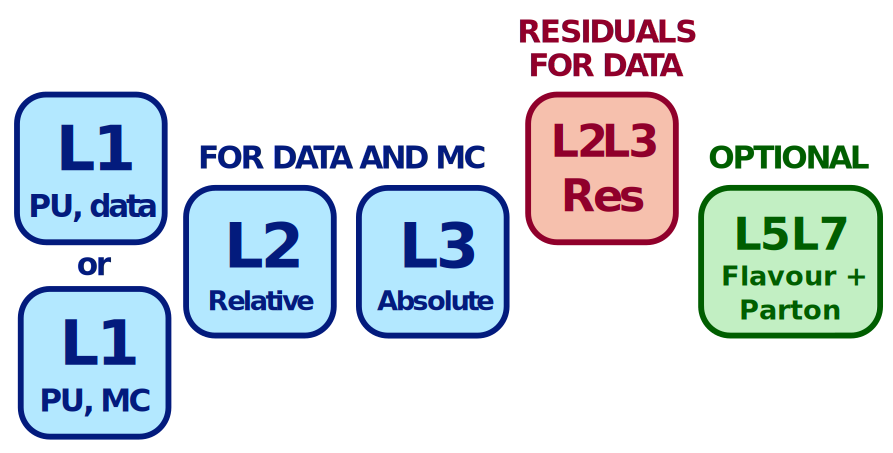
\includegraphics[width = 0.6 \textwidth]{Chapters/Chapter3/Figures/JEClevels.pdf}
 \caption{Schematical overview of the factorized approach adopted in CMS for incorporating jet energy calibrations for data and simulation (MC).}
 \label{fig::JEClevels}
\end{figure}
%The factorized approach starts by firstly removing the contribution of pileup events

\begin{myindentpar}
  \begin{description}
    \item[L1 pileup offset correction] \hfill \\
    The first contribution to the factorized correction chain aims to remove the additional energy deposits originating from pileup interactions in order to only maintain the high-$\pT$ scattering. The corresponding correction term is determined purely from simulation and is based on the average difference in transverse momentum between matched jets with and without additional pileup interactions.
    \\
    
    \indPar The offset energy needed to be subtracted from the jet energy is calculated with a \textit{hybrid jet area method}, which uses the effective area of the jets multiplied by the average energy density in the event and represents the softness of the jet activity. The full correction formula used at CMS is:    
    \begin{equation}
     \mathcal{C}_{L1}\left(\pT^{raw}, \eta, A_{j}, \rho \right) = 1 - A_{j} \dfrac{\left\lbrace \rho_{0}(\eta) + \rho . \beta(\eta) . \left[ 1 + \gamma(\eta).\log(\pT^{raw}) \right] \right\rbrace}{\pT^{raw}}
    \end{equation}
    with $\eta$ the jet pseudo-rapidity, $A_{j}$ the jet area and $\rho$ the per-event $\pT$ offset density. 
    The correction factors $\rho_{0}$, $\beta$ and $\gamma$ are determined in bins of $\eta$ by fitting the offset function using uniquely matched reconstructed jets from the with-PU sample and without-PU sample. 
    The correction formula is applied to both simulated and data events such that an additional scale factor should be taken into account in order to incorporate the small discrepancy between data and simulation.
    This scale factor is only applied for data events and is calculated from the PU-offset corrected transverse momenta of the reconstructed jets.
    %Previous studies have indicated a small discrepancy between data and simulation, which needs to be accounted for since the pileup offset correction is determined completely from simulation. Therefore an additional scale factor needs to be applied to data events to ensure that on average the energy of the reconstructed jets corresponds with the generated MC particle jets. This scale factor is multipied with the jets' PU-offset corrected transverse momenta. 
    
    \item[L2L3 Monte Carlo calibration] \hfill \\
    Now that the $\pT$-response of the jets is independent of the pileup, represented by the number of primary vertices, a following correction should be applied to ensure that the energy of the reconstructed jets corresponds - on average - with the generated jets at particle level and to obtain an $\eta^{PF}$-dependent response. This second calibration is again completely simulation-based and is determined by inverting the $\pT^{gen}$ and $\eta^{PF}$ binned response.
    \begin{equation}
     \mathcal{C}_{L2L3}(p_{\rm T, L1}^{PF}) = \dfrac{1}{\left\langle \frac{p_{\rm T, L1}^{PF}}{\pT^{gen}} \right\rangle \left(\pT^{gen}, \eta^{PF} \right)}
    \end{equation}
    The correction factors are derived from a QCD multijet sample for which a jet reconstruction identical to the one used in data is applied.
    
    \item[L2Residual data-based relative ($\eta$-dependent) correction] \hfill \\
    This first data-based calibration, abbreviated to L2Res, aims at removing the residual difference in $\eta^{PF}$-dependence between data and simulation. For this dijet events with one jet contained in the barrel ($\vert \eta \vert$ $<$ $1.3$) are used. This approach allows to correct the $\pT$ response of all jets relative to the response of central jets based on the expected $\pT$ balance between both jets in the event.
        
    \item[L3Residual data-based absolute ($\pT$-dependent) correction] \hfill \\
    After correcting the relative jet energy scale, the absolute jet energy scale should still be determined. This should only be done for central jets since the L2Res calibration ensures that these values can be used outside the barrel safely. 
    The correction factors are determined using $Z+$jet (with $Z$ $\rightarrow$ $\mu^{+}\mu^{-}$ or $e^{+}e^{-}$) and $\gamma+$jet events since this allows to exploit the precise measurement of the $Z$ and $\gamma$ as reference objects.
    \\
    The L3Res correction tackles the two main remaining differences between data and simulation: slightly lower response for data than for simulation and $\pT$-dependency for the ratio of data to simulation response. These two contributions are independent and can thus be factorized as well. The constant scale factor is determined from the very precise $Z$ $\rightarrow$ $\mu^{+} \mu^{-}+$jet events while the $\pT$-dependent correction factors are obtained by combining the response of all different decay channels in a global fit.
  \end{description}
\end{myindentpar}

Each subcorrection in this factorized approach has specific JES uncertainties which are combined into a systematic uncertainty used in physics analyses. The overall uncertainty is obtained by quadratically adding the uncertainties of each level and is dominated by the $\pT$-dependent difference in pileup offset between data and simulation, the uncertainty of the jet $\pT$ resolution and the lepton/photon scale uncertainties for the L1, L2Res and L3Res subcorrection, respectively.

\subsubsection*{Jet energy resolutions}
Besides the jet energy scale also the transverse momentum or energy resolution (JER) can be influenced by discrepancies between data and simulation. %(\textit{\textbf{Nothing here about difference wrt original configuration?}})
The measurement of the JER is performed using similar methods as applied for determining the JES, but instead of looking at the mean of the response distribution the width is considered.
The jet $\pT$ resolution is determined using QCD dijet and $\gamma+$jet events and results in an $\eta$-dependent data/MC scale factor exceeding unity~\cite{}. Hence the $\pT$ resolution is about $10 \%$ worse for data than for simulation in the barrel, a value which quickly raises to roughly $25\%$ -on average- in the endcap. In order to account for this difference, the resolution for simulation events is worsened by smearing the energy of the corrected PF jets.

\subsubsection*{Identification of b-quark jets}

Identifying the jets originating from b-quark decays consists of constructing observables in order to exploit the differences between b-quark jets and light jets. The algorithms developed for this purpose, many exist in literature, are capable of distinghuishing the event topology of interest from the large bulk of background events which only contain light-parton jets.
The different b-jet-identification or b-tagging algorithms rely on the reconstructed objects defined above although some minor optimization requirements are implied for the track selection to improve efficiency~\cite{}.
\\
One of the main b-quark jet characteristics is the relatively long lifetime of the b-hadron resulting in the presence of a displaced vertex with respect to the interaction point. Since only the tracking detectors offer the spatial resolution needed to detect the displacement between the primary and secondary vertices, they are reconstructed purely from the track collection. In order to be able to cope with multiple proton-proton interactions the tracks are required to be within a cone of $\Delta R$ $=$ $0.3$ around the jet axis, defined by the direction of the jet momentum. 
The actual reconstruction of secondary vertices is an iterative process using an adaptive vertex fit. This fit algorithm estimates the position of the vertex candidate and removes all its associated tracks from the track collection. This fit procedure is repeated until no new vertex candidates can be found. During the first iteration the interaction point is used as a constraint in order to identify the prompt\footnote{Prompt tracks are tracks originating near the pp interaction point.} tracks.

The different b-tagging algorithms existing today can be divided into two distinct categories; one which distinghuishes b-quark jets from light jets based on the track impact parameters and another based on the secondary vertices. Within this thesis only the second type of b-tagging algorithms will be considered, namely the \textit{Combined Secondary Vertex} (CSV) algorithm~\cite{}. This algorithm combines the secondary vertex information with the track-based lifetime properties. Because both characteristics are combined the algorithm is also capable of discriminating between b-quark and light-parton jets when no secondary vertex was reconstructed. In such a configuration the reduced track constraints sometimes give rise to a pseudo-vertex.
\\
The b-tagging algorithms are constructed in such a way that they should only be applied for three predefined operating points which correspond to a specific misidentification probability for light partons of roughly $10 \%$, $1 \%$ and $0.1 \%$ for an average jet $\pT$ of about $80$ $\GeV$ defined respectively as \textit{Loose}, \textit{Medium} and \textit{Tight}. In this analysis only the Tight operating point is considered (\textit{\textcolor{red}{Need to determine the efficiency percentages from the ttbar sample}})

\subsection{Missing transverse energy}\label{subsec::MET}

The vast majority of physical objects produced in particle collisions can be reconstructed from the collection of energy deposits. 
However neutrinos are the exception to the rule since they are weakly interacting and carry neutral charge. Therefore they will traverse the entire detector and escape detection rendering an accurate reconstruction rather challenging.
\\
So in order to ensure the reconstruction of neutrinos or other hypothetical neutral weakly interacting particles, a signal extremely important for many physics analyses, a specific work-around is applied which is based on indirect observations rather than direct measurements. The solution lies to a great extent in the geometrical characteristics of the particle detectors, by requiring them to be hermeticaly closed such that all other particles are propertly detected and cannot leave the detector unseen.
Thus the missing transverse momentum, which corresponds to all neutrinos and other weakly interacting neutral particles present in the event, can be defined from the total transverse momentum of all observed final-state particles~\cite{}. This procedure allows to exploit the high reconstruction efficiency of the particle-flow algorithm for the neutrino reconstruction.
\begin{equation}
 \vecmet = - \sum \vec{\pT}
\end{equation}
\textit{Calibration of $\met$}
%\textit{Some information about $\met$ resolution}\\
%\textit{Which corrections are applied ?}\\
%\textit{For which reason is $\met$ used ?}

%%\dropchapter{0.4in}
\chapter{title} \label{chp:labelTitle}
%\epigraphhead[70]{\epigraph{\textit{If I could remember the names of all these particles, I'd be a botanist.}}{Enrico Fermi}}
%\undodrop

\chapter{The Matrix Element method} \label{ch::MW}

The measurement of the right-handed tensor coupling of the Wtb interaction discussed in this thesis is performed using the Matrix Element method.
This is an advanced analysis technique which allows to extract theoretical information from experimental events without requiring prior knowledge of the possible new-physics scenarios.
%The method finds its name in the fact that 
%\textit{The Matrix Element method has been developed several years ago and has been used extensively at the Tevatron, especially in the top-quark physics sector.}
%\\
\\
The Matrix Element method assigns a probability to each theoretical hypothesis on an event-by-event basis, by calculating the matrix element of the considered process.
The obtained event probabilities are then combined into a likelihood and the most probable hypothesis is determined using a likelihood-maximisation method.
\\
\\
A detailed overview of the technicalities and applicability of the Matrix Element method can be found in this Chapter.
At first, the theoretical framework used to calculate these event probabilities will be discussed in Section~\ref{sec::MWTheory}.
In order to demonstrate the use of the Matrix Element method, the measurement of the top-quark mass will be presented as an example/feasibility study in Section~\ref{sec::MEMExample}.

\section{Theoretical framework (IMPROVE)} \label{sec::MWTheory}

The Matrix Element method has been developed several years ago in order to make maximal use of the kinematic information available.
Since this method capable of analysing processes with a complex final state, typically containing several jets and missing energy, it has been used extensively in the top-quark physics sector at the Tevatron~\cite{MEMTevatron}.
Given the challenging conditions the LHC is faced with, the use of the Matrix Element method has been revived recently and it has found applications in different physics areas; including the discovery of the Brout-Englert-Higgs boson~\cite{HiggsMEM}.
\\
\\
The fact that the Matrix Element is capable of dealing in an efficient manner with event signatures involving missing energy together with the option it provides to determine the most optimal theoretical parameter of any imposed theoretical model\footnote{The Matrix Element method also has a second widely used application, where it analyses two competing hypotheses and determines which one corresponds the most with the available experimental information.}, has made it the appropriate analysis technique to use for the measurement of the $\gR$ coefficient.
\\

Section~\ref{subsec::MWLik} will focus on the determination of the Matrix Element method and the procedure followed to calculate the matrix-elements of each event. Section~\ref{subsec::FRModel} will discuss the details of the imposed theoretical model specifically developed for the study of the anomalous couplings in the Wtb interaction vertex.

\subsection{Likelihood definition and evaluation} \label{subsec::MWLik}

The probability for each experimental event to agree with the considered theoretical model, for which the information is provided by the squared matrix-element, 
is defined as:
\begin{equation} \label{eq::MWEvtProb}
 P(x \vert \alpha) = \frac{1}{\sigma_{\alpha}} \int d\Phi(y) \, dq_{1} \, dq_{2} ~ f_{1}(q_{1}) \, f_{2}(q_{2}) \, \vert M_{\alpha}(y) \vert^{2} \, W(x,y)
\end{equation}
with $x$ the reconstructed event, $y$ the parton-level configuration, $\alpha$ the set of parameters, $\vert M_{\alpha}(y) \vert^{2}$ the squared matrix-element, d$\Phi$ the phase-space measure, $f_{i}(q_{i})$ the parton distribution functions and $W(x,y)$ the resolution or transfer function.
\\
This resolution function, which will be discussed in detail in Section~\ref{sec::TF}, ensures the detector effects influencing the reconstructed events are transfered to the parton-level configuration.
Normalising the obtained event weight with the total cross-section $\sigma_{\alpha}$ is necessary in order to obtain a probability density. Hence this should incorporate both the different cross-section values of the process and the different selection efficiency when varying the theoretical parameter $\alpha$ in the considered model. 
More detail on this normalisation procedure will be given in Section~\ref{sec::Norm}.
\\

The overall likelihood $\mathcal{L}_{MEM}$ from which the Matrix Element method will extract the most optimal value of the theoretical parameter $\alpha$, is obtained by multiplying all these individual event probabilities. The actual extraction is done by minimising these likelihood values.
\begin{equation}
 \mathcal{L}_{MEM}(x \vert \alpha) = \prod_{i=1}^{n} P(x \vert \alpha)
\end{equation}
In practice it is more convenient to convert the likelihood values using $\chi^{2}$ = $-2 \ln \mathcal{L}$ such that the log-likelihood curves of the event can be summed and that the overall $\DeltaChi$ = $\chi^{2}_{MEM} - \chi^{2}_{MEM,min}$ can be minimised. \textbf{Mention this MEM estimator stuff ...}
\begin{equation}
 \chi^{2}(x \vert \alpha) = -2 \ln \mathcal{L}_{MEM}(x \vert \alpha) = -2 \sum_{i=1}^{n} \ln P(x \vert \alpha)
\end{equation}

The Matrix Element method is supposed to provide the most powerful tool to extract theoretical information from a sample of experimental events.
However, the applicability of the method is seriously limited by the challenging computation procedure of the individual event probabilities.
The evaluation of each individual event requires a non-trivial multi-dimensional integration over the combined theoretical the hard-scattering process, and the experimental information, the transfer functions.
Hence even to analyse a limited data sample, a significant processing time has to be foreseen.
\\
\\
Due to the increasing number of possible applications of the Matrix Element method at the LHC and in phenomenological studies, a dedicated algorithm aimed at evaluating these event weights using a fully automated approach has been developed. This highly flexible phase-space generator (\textbf{not integrator?}), which uses the adaptive Monte Carlo integrator VEGAS~\cite{VEGAS}, has been denoted as MadWeight~\cite{MadWeightPaper}.
%\\
Before this tool was available, a separate integration procedure had to be developed for each considered process and detailed knowledge on the technical details of both matrix-element generation and phase-space integration was required to apply the Matrix Element method.
%\textit{This is no longer the case since the MadWeight integrator optimises the phase-space mapping.}
%***********************
% The notation of calling MadWeight a phase-space generator can be found on their twiki!!
% https://cp3.irmp.ucl.ac.be/projects/madgraph/wiki/MadWeight
%***********************
\\

%Now mention the fact that it is still slow and thus a stringent event selection has been asked for + limited the permutations of the b-jets!
Even with the implementation of the MadWeight integrator, the Matrix Element method remains a very time-consuming analysis technique.
Therefore it should be avoided to calculate the probabilities of events for which the expected final state particles are not, or incompletely, recovered; hence the stringent event-selection criteria imposed in Chapter~\ref{ch::EvtSel}.
Also the choice to distinguish the two b-quark jets originating from the W-boson decay in top-quark pair events has been applied for the purpose of reducing the necessary computing time, since this reduces the number of permutations to be considered with a factor of $2$.
Hence for this analysis, where the semi-muonic decay of the $\ttbar$ events is studied, this implies that only the permutations between the two light jets have to be performed during the integration procedure. 


\subsection{Implementation of the anomalous Wtb Lagrangian} \label{subsec::FRModel}

Since it has been opted for to implement the MadWeight integration procedure in the MadGraph framework, the option to analyse personally created theoretical models describing new-physics phenomena has been significantly facilitated.
%\textit{This approach allows to go from theory to simulation to comparison with experiment in a quick, efficient and accurate manner (Not completely own words!)}
%\\
Hence, any model can be created with FeynRules~\cite{FeynRules}, which is a Mathematica-based package to calculate Feynman rules, and be translated to MadGraph using the dedicated interface.
The developed model should only contain some basic information, such as the particle content, the parameters and the lagrangian, which allows the FeynRules package to derive the Feynman rules.
\\

In this analysis a new model has been created using this FeynRules package since no anomalous couplings for the top-quark pair decay vertex are expected in the Standard Model Lagrangian.
This so-called Wtb-model is constructed as an addition of the Standard Model, hence the entire particle content and parameters of this model has been kept.
The description of the anomalous couplings is then included by introducing four new complex parameters, the four coupling coefficients, and the full lagrangian described in Equation (\ref{eq::FullWtbLagr}).
Since the parameter of interest for this analysis, the $\gR$ coefficient of this Wtb interaction vertex, is associated with the decay of the top-quark and is thus not foreseen to change the final state particles, the particle content has not been altered.
\\
Within the model some simplifications have been added since the complexity of the developed model is directly related to the processing time needed for the MadWeight integration procedure to evaluate an event. %described by the introduced theoretical model.
Hence, the light-flavoured quarks (u-, d-, c- and s-quark) are assumed to be massless and, just as is the case for the Standard Model decays, the CKM-suppressed W-boson decays have been suppressed.
\\

Besides calculating the Feynman rules for the developed theoretical model, the FeynRules package also ensures the introduced lagrangian fulfills the basic set of requirements, such as hermicity, gauge invariance, $etc. $.
Nevertheless, the downside of developing such a brand new model is that there is no straightforward way to determine whether the obtained output for the various unknown parameters \textit{corresponds to the expectations/is well described}.
For the top-quark decay interaction vertex some influences of the coupling coefficients can be visualised by looking at the distortions of the angular distribution of the \textbf{top-quark decay products}, as has been mentioned in Section~\ref{sec::SubWtb}. 
Hence, a thorough comparison has been performed with the distributions obtained when simulating events with different values for the coupling coefficients using the developed Wtb-model, resulting in an excellent agreement as can be seen in Figure~\ref{fig::ModelTest}.
In addition, the model has also been used to calculate the most optimal value of some of the well-known parameters of the Standard Model, for which no unexpected deviations have been observed. 

\begin{figure}[h!t]
 \centering
 \includegraphics[width = 0.3 \textwidth]{image.png}
 \caption{\textbf{Comparison between theory and MadGraph model output.}} \label{fig::ModelTest}
\end{figure}


\section{Resolution functions} \label{sec::TF}

As mentioned in the previous section, the Matrix Element method uses the parton-level information extracted from the actual matrix element of the considered theoretical model to calculate the event probability.
Hence, in order to \textit{match/link} the three momenta of these final-state \textit{particles/partons} with the corresponding momenta of the reconstructed physics objects, carefully calculated resolution functions are \textit{required/needed/necessary}. 
\\
\textbf{Combined effect of parton showering, hadronisation and detector response.}
\\
\\
Nevertheless (its importance), this aspect of the Matrix Element method has some strong simplifications imposed.
Since such a resolution function should be determined for each particle type, describing both its direction ($\phi$ and $\theta$) and energy, it is assumed that these functions are uncorrelated.
This allows to reformulate the resolution function $W(x,y)$ in Equation (\ref{eq::MWEvtProb}) using a factorised approach:
\begin{equation}
 W(x,y) = \prod_{i}^{N} W(x_i, y_i) = \prod_{i}^{N} W_{i}^{E}(x^{i},y^i) \, W_{i}^{\eta}(x^i, y^i) \, W_{i}^{\phi}(x^i,y^i)
\end{equation}
where the index $i$ runs over the different types of physics objects in the considered event topology.
\\
\\
This \textit{factorised} description can be simplified even further since (\textit{the transfer functions of}) both object directions can be respresented with a Dirac-$\delta$ function.
This because both angles are determined very precisely (\textit{in the CMS detector/hadron detectors}) and therefore correspond very well with the measured objects, as can be seen from Figure~\ref{fig::TFAngles}. The differences shown in these distributions are determined using the parton-level and reconstructed physics object to have an angular distance $\Delta R$ smaller than 0.3, a similar condition as what is applied in Chapter~\ref{ch::EvtSel}.
As a result, the only remaining phase-space variable for which a transfer function should be determined is the energy, for which the introduced assumption is not correct due to the finite resolution on its measurement. The transfer function of the energy variable will therefore be represented with a Gaussian-like function.
\\
\begin{figure}[h!tp]
 \centering
 \includegraphics[width = 0.31 \textwidth]{image.png} \hspace{0.1cm} 
 \includegraphics[width = 0.31 \textwidth]{image.png} \hspace{0.1cm}
 \includegraphics[width = 0.31 \textwidth]{image.png}
 \caption{Draw the $\Delta \phi$ and $\Delta \theta$ to show this is very narrow! + Show difference with $\Delta E$. (Kinematic variables are the ones with all corrections as discussed in Chapter~\ref{ch::EvtSel})} \label{fig::TFAngles}
\end{figure}

In this analysis, which focusses on the semi-muonic decay of top-quark pairs, a dedicated transfer function should be developed for the jets and the muon in the event.
However, due to the possible different behaviour of the light- and heavy-flavoured jets, it has been opted for to determine two separate transfer functions for the jets.
Hence, the two jets identified as originating from the decay of the W-boson and the two jets assigned to the b-quark decay will be treated independently. 
The transfer function for the muons on the other hand will also be represented with a Dirac-$\delta$ function since its energy is determined very precisely. The different behaviour for the muon and the jets, the light-flavoured ones in this case, can be seen in Figure~\ref{fig::TFJetEDistr}.
%\textit{Looking at the energy difference for the muons also indicated that this is actually determined very precisely and can therefore also be respresented with a Dirac-$\delta$ function.}
\\
Besides simplifying the transfer-function calculation, this approach of using Dirac-$\delta$ functions for various phase-space variables and particles also significantly speeds up the Matrix Element method.
Fixing the properties of the reconstructed objects to those of the parton-level ones implies that the method does not have to integrate over the corresponding phase-space variables.
%*****************************************
% This non-integration is mentioned on page 3 of main MadWeight paper (discusses there the ideal case of no TF)
%*****************************************
\\
\begin{figure}[h!tp]
 \centering
 \includegraphics[width = 0.3 \textwidth]{image.png} \hspace{0.2cm}
 \includegraphics[width = 0.3 \textwidth]{image.png} \\ \vspace{0.2cm}
 \includegraphics[width = 0.3 \textwidth]{image.png} \hspace{0.2cm}
 \includegraphics[width = 0.3 \textwidth]{image.png}
 \caption{$Delta E$ distributions for different parton energies.} \label{fig::TFJetEDistr}
\end{figure}

The transfer function of the both the light- and heavy-flavoured jets will be described using a double-Gaussian distribution, for which the formula is given in Equation (\ref{eq::DblGausTF}).
%The factor $(a_2 + a_3 a_5)$ ensures the obtained transfer function is normalised such that the event-probability remains a probability density.
This double-Gaussian representation is the optimal choice to describe the energy difference ($\Delta E$ = $E_{parton}$ - $E_{jet}$) of jets, which is characterised by a sharp peak combined with an asymmetric tail. 
From Figure~\ref{fig::TFJetEDistr} can furthermore be concluded that the width of the overall $\Delta E$ distribution increases for higher energies of the matched parton. Hence an accurate description of both the peak and the tail is necessary in order to ensure the transfer function remains valid for a wide energy regime.
\begin{equation} \label{eq::DblGausTF}
 W^{E}(parton, jet) = \frac{1}{\sqrt{2\pi}} \frac{1}{a_2 + a_3 a_5} \left( \exp \frac{-(\Delta E - a_1)^2}{2 a_2 \,^{2}} + a_3 \exp \frac{-(\Delta E - a_4)^2}{2 a_5 \,^{2}} \right) 
\end{equation}
where the parameters $a_1$ and $a_4$ represent the mean of the first and second Gaussian, respectively, while the parameters $a_2$ and $a_5$ give the width of those respective Gaussian distributions.
The remaining parameter $a_3$ takes into account the relative contribution of both distributions.
\\

The actual determination of the two remaining transfer functions will be performed by applying a double-Gaussian fit on the obtained $\Delta E$ distribution for various $E_{parton}$ values.
For the light jets 16 bins are considered between $25 \GeV$ and $160 \GeV$, while for the b-quark jets 18 bins are used between $30 \GeV$ and $230 \GeV$.
In order to ensure sufficient statistics is available throughout the entire energy-range, only the basic event-selection requirements have been applied. So the fine-tuning criteria discussed in Section~\ref{sec::SpecificSelec} are not taken into account when determining the transfer functions.
\\
Hence for each of the considered $E_{parton}$-bins a measurement of the five $E$-dependent parameters representing the double-Gaussian transfer function is obtained.
The $E$-dependency of these transfer-function parameters is based on the parametrisation of the calorimeter energy resolution, which corresponds to $y$ = $a + b \sqrt{E} + c E$.
However, in order to ensure the parameters are well described by this parameterisation, a quadratic term, or for some parameters even a cubic term, has been added. An overview of the imposed $E$-dependency for the different $a_i$ parameters can be found in Table~\ref{table::EDependency}.
\\
\begin{table}[h!tp]
 \centering
 \caption{Imposed $E$-dependency of the different transfer-function parameters. Only in three cases the additional cubic function was necessary to obain a good description of the corresponding parameter.} \label{table::EDependency}
 \renewcommand{\arraystretch}{1.2}
 \begin{tabular}{|c|c|}
  \hline
  Light-jet parameters 								& b-quark jet parameters 							\\
  \hline
  $a_{1,0} + a_{1,1}\sqrt{E} + a_{1,2} E + a_{1,3} E^{2} + a_{1,4} E^{3}$ 	& $a_{1,0} + a_{1,1}\sqrt{E} + a_{1,2} E + a_{1,3} E^{2} + a_{1,4} E^{3}$ 	\\
  $a_{2,0} + a_{2,1}\sqrt{E} + a_{2,2} E + a_{2,3} E^{2}$ 			& $a_{2,0} + a_{2,1}\sqrt{E} + a_{2,2} E + a_{2,3} E^{2}$		 	\\
  $a_{3,0} + a_{3,1}\sqrt{E} + a_{3,2} E + a_{3,3} E^{2}$		 	& $a_{3,0} + a_{3,1}\sqrt{E} + a_{3,2} E + a_{3,3} E^{2} + a_{3,4} E^{3}$ 	\\
  $a_{4,0} + a_{4,1}\sqrt{E} + a_{4,2} E + a_{4,3} E^{2}$		 	& $a_{4,0} + a_{4,1}\sqrt{E} + a_{4,2} E + a_{4,3} E^{2}$		 	\\
  $a_{5,0} + a_{5,1}\sqrt{E} + a_{5,2} E + a_{5,3} E^{2}$		 	& $a_{5,0} + a_{5,1}\sqrt{E} + a_{5,2} E + a_{5,3} E^{2}$ 			\\
  \hline
 \end{tabular}
\end{table}

The two-dimensional histogram showing the $E_{parton}$ distribution with respect to the $\Delta E$ distribution for both the light- and heavy-flavoured jets can be found in Figure~\ref{fig::TF2DPlot}, respectively the left and right plot.
Comparing the two distributions allows to conclude that it is indeed beneficial to treat both types of jets independently since a wider $\Delta E$ distribution is clearly visible for the b-quark jets.
\\
Figure~\ref{fig::TFSlices} contains some examples of the $\Delta E$ distribution obtained for some specific parton-level energy bins. The two upper plots correspond to the light-flavoured jets while the two lower ones depict the situation for the heavy-flavoured ones.
In order to visualise the importance of using a double-Gaussian description for the transfer functions of the jet energies, the left distribution gives the distribution for the relatively low parton energies while the right corresponds to one of the more outer bins of the considered energy range.
As can be seen, the range where the double-Gaussian fit is applied has been optimised for each of the considered bins of $E_{parton}$.

\begin{figure}[h!tp]
 \centering
 \includegraphics[width = 0.45 \textwidth]{Chapters/Chapter5_MadWeight/Figures/Light_DiffEVsGenE.pdf} \hspace{0.2cm}
 \includegraphics[width = 0.45 \textwidth]{Chapters/Chapter5_MadWeight/Figures/BJet_DiffEVsGenE.pdf} 
 \caption{Two-dimensional histogram showing the parton energy $E_{parton}$ with respect to the difference in energy with the matched jet, $\Delta E$ for the light jets (left) and the b-quark jets (right). The transfer-function is determined from these histograms by fitting the $y$-axis projection of each considered $x$-axis bin with a double-Gaussian.} \label{fig::TF2DPlot}
\end{figure}

\begin{figure}[h!tp]
 \centering
 \includegraphics[width = 0.45 \textwidth]{Chapters/Chapter5_MadWeight/Figures/sliceYbin2And3_Light_DiffEVsGenE.pdf} \hspace{0.2cm}
 \includegraphics[width = 0.45 \textwidth]{Chapters/Chapter5_MadWeight/Figures/sliceYbin12And13_Light_DiffEVsGenE.pdf} \vspace{0.1cm} \\
 \includegraphics[width = 0.45 \textwidth]{Chapters/Chapter5_MadWeight/Figures/sliceYbin3_BJet_DiffEVsGenE.pdf} \hspace{0.2cm}
 \includegraphics[width = 0.45 \textwidth]{Chapters/Chapter5_MadWeight/Figures/sliceYbin12And14_BJet_DiffEVsGenE.pdf}
 \caption{Distribution of the difference in energy between the parton-level and reconstructed object for both the light jets (upper two) and the b-quark jets (lower two) fitted with a double-Gaussian function. The different shape for lower (left) and higher (right) energy values is clearly visible.} 
\end{figure}

Finally, the obtained $E$-dependent shape of the five parameters describing the double-Gaussian transfer function is given in Figure~\ref{fig::TFLight} and \ref{fig::TFBJet} for the light and b-quark jets, respectively. In case some of the considered $\Delta E$ distributions was low on statistics, it has been combined with one of the surrounding bins in order to ensure sufficient information was available for the double-Gaussian fit.
This effect is clearly visible in the depicted measurement points, especially at the edges of the considered energy range where the number of events started to decrease.

\begin{figure}[h!tp]
 \centering
 \includegraphics[width = 0.46 \textwidth]{Chapters/Chapter5_MadWeight/Figures/Light_DiffEVsGenE_a1_Fit.pdf} \hspace{0.2cm}
 \includegraphics[width = 0.46 \textwidth]{Chapters/Chapter5_MadWeight/Figures/Light_DiffEVsGenE_a2_Fit.pdf} \vspace{0.3cm} \\
 \includegraphics[width = 0.46 \textwidth]{Chapters/Chapter5_MadWeight/Figures/Light_DiffEVsGenE_a3_Fit.pdf} \hspace{0.2cm}
 \includegraphics[width = 0.46 \textwidth]{Chapters/Chapter5_MadWeight/Figures/Light_DiffEVsGenE_a4_Fit.pdf} \vspace{0.3cm} \\
 \includegraphics[width = 0.46 \textwidth]{Chapters/Chapter5_MadWeight/Figures/Light_DiffEVsGenE_a5_Fit.pdf}
 \caption{Obtained shape for the five $E$-dependent parameters describing the double-Gaussian transfer function for the light-flavoured jets. This has been fitted with the corresponding parametrisation given in Table~\ref{table::EDependency}.} \label{fig::TFLight}
\end{figure}

\begin{figure}[h!tp]
 \centering
 \includegraphics[width = 0.46 \textwidth]{Chapters/Chapter5_MadWeight/Figures/BJet_DiffEVsGenE_a1_Fit.pdf} \hspace{0.2cm}
 \includegraphics[width = 0.46 \textwidth]{Chapters/Chapter5_MadWeight/Figures/BJet_DiffEVsGenE_a2_Fit.pdf} \vspace{0.2cm} \\
 \includegraphics[width = 0.46 \textwidth]{Chapters/Chapter5_MadWeight/Figures/BJet_DiffEVsGenE_a3_Fit.pdf} \hspace{0.2cm}
 \includegraphics[width = 0.46 \textwidth]{Chapters/Chapter5_MadWeight/Figures/BJet_DiffEVsGenE_a4_Fit.pdf} \vspace{0.2cm} \\
 \includegraphics[width = 0.46 \textwidth]{Chapters/Chapter5_MadWeight/Figures/BJet_DiffEVsGenE_a5_Fit.pdf}
 \caption{Obtained shape for the five $E$-dependent parameters describing the double-Gaussian jet transfer function for the b-flavoured jets. This has been fitted with the corresponding parametrisation given in Table~\ref{table::EDependency}.} \label{fig::TFBJet}
\end{figure}

~~~

%Due to the introduced assumptions, the applicability of the Matrix Element method will need to be tested in detail in order to ensure it is not affected by a bias, as will be discussed in Section~\ref{sec::EstimatorProp}.
%\\
%\textit{But in my case linearity test is not performed using the Transfer Functions discussed here!!}

\section{Cross-section  normalisation} \label{sec::Norm}
\textit{Since it is here a rather general case, first the method for generator-level events can be mentioned and then the difference with reconstructed collision events can be made perfectly clear.}

An important aspect of the Matrix Element method is the normalisation of the event probability using the cross-section and acceptance, which might vary significantly for the considered configurations. For the top-quark mass example given in Section~\ref{sec::TopMass}, the effect of this normalisation was negligible but for the measurement of the anomalous coupling coefficient this factor has proven to be rather important. The method opted for in this analysis to determine these cross-section values will be explained in Section~\ref{subsec::XSReco}.

For the measurement of the right-handed tensor coupling the cross-section normalisation is a vital component.
Independent whether generator-level or reconstructed events are considered, without this normalisation applied the Matrix Element method does not result in the correct outcome.
The substantial influence of this normalisation component has been summarised in Figure~\ref{fig::XSInflGen}, which shows the overall $\chiSqMEM$ distribution prior to and after the cross-section normalisation has been taken into account. The considered sample has been created using the Standard Model configuration such that the minimum of the distribution should correspond to $0$.
%This because the observed variations of the overall event probability for the coupling coefficient are much smaller than was the case for the top-quark mass measurement such that the cross-section normalisation actually has a significant influence on the obtained outcome.
%***********************************
% --> Certain this is the reason?
% ==> Maybe good to think of an explanation why this cross-section normalisation is so much more important
%***********************************
\begin{figure}[h!t]
 \centering
 % Add here the gR gen-level result of FitDistributions_CalibCurve_SemiMu_RgR_AllDeltaTF_MGSampleSM_20000Evts_NoCuts_OuterBinsExclForFit_20000Evts.root with and without XS normalisation
 % Important: Cannot yet use the sample after the event-selection is applied because this still has to be explained!!
 % --> Do this without the fit maybe .. ?
 \includegraphics[width = 0.3 \textwidth]{image.png} \hspace{0.5cm}
 \includegraphics[width = 0.3 \textwidth]{image.png}
 \caption{Distribution of the overall $\chiSqMEM$-value obtained by analysing the right-handed tensor coupling using 20 000 generator-level events. The distribution on the left is without any normalisation applied while the right one corresponds to the normalised result.} \label{fig::XSInflGen}
\end{figure}

The significant impact of the cross-section normalisation on the outcome of the measurement implies that the cross-section values for the reconstructed-level analysis should be determined with great care.
However, in contrast to the easy access to generator-level samples with alternative coupling coefficients, generating similar samples containing reconstructed events is a rather challenging and time-consuming process.
As a result, it has been opted for in this thesis to derive the cross-section values for the reconstructed events from the generator-level ones.
This approach significantly facilitates the cross-section determination since any generated process by MadGraph automatically calculates the cross-section of the considered process.
%**********************
% Any other motivation why FastSim has not been considered?
% --> Certain that it would perfectly describe the SM samples??
%**********************
\\
\\
In order to ensure that the obtained generator-level cross-sections can easily be related to the reconstructed ones, the conditions present for the reconstructed collision events will be mimicked as closely as possible during the generation process. Hence the generator events have to fullfill the basic event selection requirements\footnote{Important to note here is that once these selection criteria are applied to the generated events, the obtained cross-section will actually be a combination of the cross-section of the underlying physics process and the acceptance of the considered event selection. Hence the term ``cross-section normalisation'' will \textbf{implicitely} imply the combined normalisation $\sigma \times A$ mentioned in Equation~\ref{eq::MWEvtProb}.} listed in Table~\ref{table::GenCuts}.
By applying a significant fraction of the full event selection chain onto the generated events, the expected relative difference in behaviour of each $\gR$ value on the considered kinematic constraints will be incorporated. As previously mentioned in Section~\ref{sec::CalibCurve}, the remaining event-selection criteria are supposed to be less sensitive to the value of the coupling coefficient.
%The remaining event selection criteria are believed to be less sensitive to the value of the coupling coefficient, thus their relative dependence will not be taken into account.
\\
\\
In addition, the generated processes are also selected in order to remain with a similar event signature as is the case in data. Hence the cross-section values have been determined using a combination of top-quark pair decay processes surrounded with additional jets. The actual number of considered processes has been limited to the $\ttbar$ decay with none, one and two additional jets since the contribution of the following decays quickly becomes negligible.
%********************************************
% --> Does this correspond to LO, NLO and NNLO or is this still something different??
% Question: Interesting to give some of the Feynman diagrams belonging to the different processes?
%********************************************
\begin{figure}[h!t]
 \centering
 \includegraphics[width = 0.15 \textwidth]{image.png} \hspace{0.2cm}
 \includegraphics[width = 0.15 \textwidth]{image.png} \hspace{0.2cm}
 \includegraphics[width = 0.15 \textwidth]{image.png}
 \caption{Feynman diagrams for the different generator-level processes considered for the calculation of the cross-sections. \textbf{Relevant?}}
\end{figure}

Even with these two optimisations applied, this approach will not result in a perfect agreement with the selected events. For instance, it is simply not possible to include every aspect of the full event-selection chain in exactly the same way when generating the different processes.
Hence, the obtained cross-section values will be scaled in order to take into account the influence of these non-included event selection criteria.
For this an identical behaviour throughout the entire $\gR$ range is assumed such that each cross-section value will be multiplied with the factor $\sigma_{SM}^{reco}$/$\sigma_{SM}^{gen}$. 
%********************************************
% --> Think of any other non-included effects!!
%********************************************
\\
In this factor the term $\sigma_{SM}^{reco}$ represents the measured cross-section of the selected events while the cross-section obtained for the combined generator-level sample created using the Standard Model configuration is denoted by $\sigma_{SM}^{gen}$.
The cross-section of the selected events is determined by dividing the semi-leptonic $\ttbar$ event count obtained after the full event selection chain with the luminosity of this sample, which has been given previously in Table~\ref{table::Samples}. 
\\

The final result of the cross-section calculation can be found in Figure~\ref{fig::XSDistr}, which shows the distribution of the cross-section values obtained for the generator-level events using the approach discussed above. The cross-section values for the selected events are also given in this Figure, obtained by multiplying each of the former cross-sections with the fixed scaling factor $\sigma_{SM}^{reco}$/$\sigma_{SM}^{gen}$ = $0.134$.
\\
\textbf{Remark: Used luminosity and number of events do not seem to be correct!}
\begin{figure}[h!t]
 \centering
 \includegraphics[width = 0.7 \textwidth]{Chapters/Chapter5_MadWeight/Figures/DerivedXSDistribution_gRCoefficient.pdf}
 \caption{Overview of the distribution of the generator-level cross-sections for different $\gR$ values and the reconstructed ones derived from them by applying the ratio $\sigma_{SM}^{reco}$/$\sigma_{SM}^{gen}$.} \label{fig::XSDistr}
\end{figure}

%--------------------------------------------------------------------------------------------------------- \\
%Also here there is an additional complexity when considering reconstructed events, since the cross-section of the $\ttbar$ decay depends on the value of the coupling coefficients in the interaction vertex. For generator-level events, these values are accesible for each generated sample since MadGraph automatically determines the cross-section of each generated process.
%\\
%Hence the cross-sections for these reconstructed events are derived from the MadGraph predictions by carefully calculating the generator-level cross-sections in a regime comparable to data. 
%This condition has been achieved by combining the cross-sections for each $\gR$ coefficients when no, one and two additional jets are included in the event. 
%This will not result in a perfect match to data, but will bring the considered configuration a bit closer to reality. 
%\\
%Since the cross-section should be include the effect of the event selection, the different MadGraph samples have to fullfill the different kinematic requirements given in Table~\ref{table::GenCuts}. The three different contributions are then added in order to obtain an overall cross-section for the \textbf{inclusive} 2-jet case, for which the results have been summarised in the second column of Table~\ref{table::XSValues}.
%The third column contains the cross-section values that will be applied for the measurement using the reconstructed events, and have been obtained by scaling the cross-section for each $\gR$ value with the fraction $\sigma_{SM}^{reco}$/$\sigma_{SM}^{gen}$. This ratio corrects the generator-level cross-sections to the expected reco-level one and can be applied onto all $\gR$ configurations since the relative effect of the event selection is already been incorporated by applying the basic event selection requirements on the MadGraph samples. The value $\sigma_{SM}^{reco}$ has been determined by dividing the number of selected events with the total number of events present in the sample and multiplying this with the cross-section of the semi-leptonic $\ttbar$ sample, which thus corresponds to multiplying the selected number of events with the luminosity of the simulated sample. The distribution of the generator-level cross-sections and the reconstructed ones is given in Figure~\ref{fig::XSDistr} and serves as an easy way to determine the reconstructed cross-section for other $\gR$ values if required.

\section{The Matrix Element method in practice} \label{sec::MEMExample}   %Practical application of the Matrix Element method

In order to apply the Matrix Element method, or more specifically the MadWeight integration procedure, the experimental information should be provided in a predefined format. For each particle in the event topology, including the missing energy representing the neutrino, the transverse momentum, the pseudo-rapidity, the azimuthal angle and the mass should be given.
The transverse momentum is then internally converted into a transverse energy, using the provided mass value, to ensure the available phase-space information can be accessed by the transfer functions.
\\
The actual integration procedure is performed in a straightforward manner and can be applied on any parameter described by the considered theoretical model. 
The different parameter values that need to be calculated have to be specified, and the integration procedure will then provide an event probability for each of these parameter values.
%The corresponding weight that is obtained from this integration procedure is merely a representation of the integration procedure and can not be used
\\
\\
Unfortunately for a tiny fraction of events the integration procedure fails to converge and is thus not capable of providing an event probability. 
In some cases this occurs for merely one of the considered parameter values, but nevertheless the entire event should be excluded in order to avoid having a biased overall likelihood.
This is however not a significant effect since even for the most affected sample, this corresponds to less than $0.7\%$ of the events in this analysis.
It has been ensured that the data sample is unaffected by this feature and thus has the full statistics available.
\\

The practical application of the Matrix Element method will be demonstrated by measuring the top-quark mass, a parameter for which this advanced technique has been used extensively.
Since the top-quark mass is accurately determined in the Standard Model, this measurement allows to observe any possible bias which can be introduced by applying this procedure.
The measurement has been performed both on generator-level events and on a limited number of simulated $\ttbar$ events fulfilling the full list of event-selection criteria discussed before.
\\
%In order to ensure the reconstructed events bear sufficient information to perform the measurement using the limited statistics, 
%In order to ensure the considered events had sufficient information for providing an accurate measurement, the study of the reconstructed events has been restricted to $\ttbar$ events for which each jet in the reconstructed event topology has been correctly matched with the corresponding parton.
Since this measurement serves merely as an illustrative example, the study of the reconstructed events will be restricted to $4000$ $\ttbar$ events for which each jet in the reconstructed event topology has been correctly matched with the corresponding parton. 
The resolution functions applied for the generator-level events have been significantly simplified by restricting all of them to a Dirac-$\delta$ function while for the reconstructed events the ones discussed in Section~\ref{sec::TF} will be applied.
Six different values of the top-quark mass have been scanned over between $170 \GeV$ and $175\GeV$. \textbf{Change range?}
%\textit{Hence, this will allow to obtain an accurate top-quark mass measurement with the considered limited statistics.}
\\
\\
Before the actual measurement of the top-quark mass can be performed, the cross-section values for the reconstructed events have to be determined following the same procedure as explained in Section~\ref{sec::Norm}. The obtained results is shown in Figure~\ref{fig::XSDistrTop} and clearly indicates that the top-quark mass depends less heavily on the cross-section than the $\gR$ coefficient in Figure~\ref{fig::XSDistr}. 
\textit{This implies that the importance of this cross-section normalisation is less significant for the measurement of the top-quark mass and that an incorrect determination will influence the overall result less.}
\\
\begin{figure}[h!t]
 \centering
 \includegraphics[width = 0.7 \textwidth]{Chapters/Chapter5_MadWeight/Figures/DerivedXSDistribution_TopMass.pdf}
 \caption{Overview of the distribution of the generator-level cross-sections for different top-quark mass values and the reconstructed ones derived from them by applying the ratio $\sigma_{SM}^{reco}$/$\sigma_{SM}^{gen}$.} \label{fig::XSDistrTop}
\end{figure}

The strenght of the Matrix Element method finds its origin in the fact that it analyses each event individually, assigns a probability to corresponds with the presumed hypothesis and then combines this information into one overall likelihood.
Hence events for which the reconstructed event topology and kinematic information corresponds well with the considered process will therefore contain the most relevent information and are supposed to contribute on average the most to the overall result.
\\
The difficulty of extracting information on an event-by-event basis can be visualised in Figure~\ref{fig::EvtProbsMTGen} where a number of event probabilities are shown for the top-quark mass measurement using generator-level events. The upper row contains events exhibiting the expected behaviour while the individual likelihood values in the middle row clearly indicate that the corresponding event has very little relevant information on the theoretical assumption.
Nevertheles, the Matrix Element method is capable of combining all the separate event probabilities into a overall likelihood from which the theoretical parameter will be extracted. This overall likelihood is shown as the bottom plot. % in Figure~\ref{fig::EvtProbsMTGen}.
\\
\begin{figure}[h!tb]
 \centering
 \includegraphics[width = 0.31 \textwidth]{Chapters/Chapter5_MadWeight/Figures/EventLikelihood_MG_4000Evts_AllDeltaTF_150.pdf} \vspace{0.2cm}
 \includegraphics[width = 0.31 \textwidth]{Chapters/Chapter5_MadWeight/Figures/EventLikelihood_MG_4000Evts_AllDeltaTF_450.pdf} \vspace{0.2cm}
 \includegraphics[width = 0.31 \textwidth]{Chapters/Chapter5_MadWeight/Figures/EventLikelihood_MG_4000Evts_AllDeltaTF_1450.pdf} \hspace{0.1cm} \\
 \includegraphics[width = 0.31 \textwidth]{Chapters/Chapter5_MadWeight/Figures/EventLikelihood_MG_4000Evts_AllDeltaTF_775.pdf} \vspace{0.2cm}
 \includegraphics[width = 0.31 \textwidth]{Chapters/Chapter5_MadWeight/Figures/EventLikelihood_MG_4000Evts_AllDeltaTF_1675.pdf} \vspace{0.2cm}
 \includegraphics[width = 0.31 \textwidth]{Chapters/Chapter5_MadWeight/Figures/EventLikelihood_MG_4000Evts_AllDeltaTF_3975.pdf} \hspace{0.1cm} \\
 \includegraphics[width = 0.4 \textwidth]{Chapters/Chapter5_MadWeight/Figures/OverallLikelihoodCurve_NoFit_MG_4000Evts_AllDeltaTF.pdf}
 \caption{Individual event probabilities for the measurement of the top-quark mass (upper two rows) using generator-level events, which get combined into the overall likelihood (bottom) from which the most optimal top-quark mass value can be extracted.} \label{fig::EvtProbsMTGen}
\end{figure}

The most optimal value of the considered theoretical parameter is obtained by minimising the negative logarithmic likelihood values of the full collection of experimental events.
This is done by fitting the $\DeltaChi$ values with a quadratic function on a predefined range and the obtained minimum value then corresponds to the outcome of the theoretical parameter.
\\
It has been investigated whether an improvement can be observed in case each event likelihood is fitted with such a quadratic function. The overall likelihood values is then determined by adding the individual functions instead of adding the likelihood values. 
The main advantage of this approach is that it would reduce the risk of influencing the overall outcome when one parameter value is badly calculated for a specific event. Hence, using the fitted shape would allow to extract the general shape of the likelihood values from each and be less dependent of one failing integration.
Unfortunately, due to the large statistical fluctuations present for each event and the generally small difference between the likelihood values, the shape of the individual likelihood values can not be described properly by such a quadratic function.
\\
\\
Applying the developed minimisation procedure on the $\DeltaChi$ values obtained for the top-quark measurement using generator-level events, for which the range is limited between $171 \GeV$ and $175 \GeV$, results in an outcome of the Matrix Element estimator of $173.82 \pm 0.64 \GeV$.
%For the example of the top-quark mass measurement the range has been restricted between $171 \GeV$ and $175 \GeV$ resulting in a top-quark mass of $m_{t}$ = $173.82 \pm 0.64 \GeV$ for the generator-level events. 
Since these events have been generated with MadGraph by assuming a top-quark mass of $173 \GeV$ this procedure results in a nice agreement, especially considering the limited statistics available.
\\
\begin{figure}[h!tb]
 \centering
 \includegraphics[width = 0.45 \textwidth]{Chapters/Chapter5_MadWeight/Figures/OverallLikelihoodCurve_MG_4000Evts_AllDeltaTF.pdf}
 \caption{$\DeltaChi(x_{gen} \vert m_{t})$ curve obtained for $4000$ generator-level events created in MadGraph with $m_{t}$ $=$ $173 \GeV$ fitted with a quadratic function. Minimisation this function results in a top-quark mass value of $173.82 \pm 0.64 \GeV$.}\label{fig::FitMTGen}
\end{figure}

The same procedure has then been applied to the reconstructed events, for which a similar behaviour of the individual event likelihoods exists as shown in Figure~\ref{fig::EvtProbsMT}.
Minimising the overall $\DeltaChi$ results in an outcome of this Matrix Element estimator of $173.82 \pm 0.64 \GeV$.
This deviates slightly from the top-quark mass used in the simulated events, defined as $172.5 \GeV$, which can be explained by both the limited statistics and the more challenging conditions existing for reconstructed events. Hence in order to ensure the obtained value of the Matrix Element estimator can be trusted when considering reconstructed events, a dedicated calibration procedure should be performed as  will be discussed in Chapter~\ref{ch::Analysis} for the measurement of the right-handed tensor coupling.
Nevertheless, taking into account the large statistical uncertainty and the different systematic effects likely to influence the obtained top-quark mass measurement, this feasibility study has proven that the Matrix Element method is capable of providing very precise and accurate results.
\begin{figure}[h!tb]
 \centering
 \includegraphics[width = 0.31 \textwidth]{Chapters/Chapter5_MadWeight/Figures/EventLikelihood_TTSemiLept_4000Evts_1450.pdf} \vspace{0.2cm}
 \includegraphics[width = 0.31 \textwidth]{Chapters/Chapter5_MadWeight/Figures/EventLikelihood_TTSemiLept_4000Evts_2025.pdf} \vspace{0.2cm}
 \includegraphics[width = 0.31 \textwidth]{Chapters/Chapter5_MadWeight/Figures/EventLikelihood_TTSemiLept_4000Evts_3325.pdf} \hspace{0.1cm} \\
 \includegraphics[width = 0.31 \textwidth]{Chapters/Chapter5_MadWeight/Figures/EventLikelihood_TTSemiLept_4000Evts_875.pdf} \vspace{0.2cm}
 \includegraphics[width = 0.31 \textwidth]{Chapters/Chapter5_MadWeight/Figures/EventLikelihood_TTSemiLept_4000Evts_2300.pdf} \vspace{0.2cm}
 \includegraphics[width = 0.31 \textwidth]{Chapters/Chapter5_MadWeight/Figures/EventLikelihood_TTSemiLept_4000Evts_3925.pdf} \hspace{0.1cm} \\
 \includegraphics[width = 0.4 \textwidth]{Chapters/Chapter5_MadWeight/Figures/OverallLikelihoodCurve_TTSemiLept_4000Evts.pdf}
 \caption{Individual event probabilities for the measurement of the top-quark mass (upper two rows) using reconstructed events, which get combined in the overall likelihood (last row) from which the most optimal value of the top-quark mass is extracted.} \label{fig::EvtProbsMT}
\end{figure}

\chapter{Measurement of anomalous couplings in top-quark pair decays} \label{ch::Analysis}

The technicalities of the Matrix Element method have been described in detail in Chapter~\ref{ch::MW} and will now be put to use in order to measure the anomalous couplings in the Wtb interaction vertex.
The main idea behind this advanced technique consists of combining individual event probabilities into an overall $\DeltaChi$ curve from which the considered theoretical parameter can be extracted.
%The main idea of the Matrix Element method, combining individual events probabilities into an overall negative log likelihood $\NegLL$, has been demonstrated with the simplified example of the top-quark mass determination.
This Matrix Element estimator is obtained by minimising this curve, and is denoted as $\gREst$ for the measurement of the right-handed tensor coupling.
%The main idea of the Matrix Element method is that it combines all the individual event probabilities into an overall likelihood $\mathcal{L}_{MEM}$.
%This likelihood distribution is then transformed into a negative log likelihood, which is minimized in order to extract the Matrix Element estimator $\hat{\epsilon}_{MEM}$.
%In this chapter, which will focus on the measurement of the right-handed tensor coupling of the Wtb interaction vertex, the estimator of interest is denoted as $\gREst$.
However, before the actual measurement can be performed, a number of tests have to be carried out in order to ensure the Matrix Element estimator is behaving properly.
\\
%***********************
% Repeat MEM likelihood equation??
%***********************
\\
The performance of the Matrix Element estimator has to be studied carefully since the Matrix Element method is likely to be influenced by the various assumptions and simplifications that have been introduced.
These might influence the outcome of this estimator in such a way that it significantly deviates from the correct result.
%Some of these simplifications might cause the value of this estimator to significantly deviate from the actual outcome expected from the Matrix Element method.
As a result, a detailed investigation of the correspondence between the estimator and expectation has been performed and will be discussed in Section~\ref{sec::EstimatorProp}.
%Investigating the performance of the Matrix Element estimator, explained meticulously in Section~\ref{sec::EstimatorProp}, is crucial since the Matrix Element method can be influenced by the introduced simplifications/assumptions.
%the sometimes simplified \textit{representations}.
%Determining the correspondence between the result obtained from the Matrix Element estimator and the expected $\gR$-value will be done using simulated samples, for which the Standard Model configuration should be recovered.
%
%In the ideal case, the estimator $\hat{g_{R}}$ should be identical to the $\gR$ value extracted from the event-likelihood. 
%Nevertheless, this perfect behaviour can be influenced by ... (\textit{What can be responsible for a slope different from 1? Is it also just a bias?}) and result in a ... or a bias.
%
Once the required calibrations have been identified, the developed procedure to determine the Matrix Element estimator can be applied on the collision events collected by the CMS detector.
The final results obtained for the measurement of the right-handed tensor coupling of the Wtb interaction will be given in Section~\ref{sec::gRMeas}.

\section{Performance of the Matrix Element estimator} \label{sec::EstimatorProp} %Is method needed here? --> Otherwise call it 'Performance of the estimator $\hat{g_{R}}$'

In order to ensure that the Matrix Element method behaves accordingly and results in the correct outcome, the estimator will first be determined using simulated events.
For these types of events, which have been generated using the Standard Model configuration, the expected outcome should be fixed by definition. 
Hence in case any deviation from the Standard Model expectations is observed for the outcome of the Matrix Element estimator, the developed procedure has to be calibrated.
%Hence any discrepancy between the value obtained for the Matrix Element estimator and the Standard Model ($\gR$ = 0) implies the developed procedure needs to be calibrated.
\\
Such a discrepancy does not hamper the applicability of the Matrix Element method, but simply implies that its outcome should be corrected for the observed non-optimal behaviour.
%The presence of such a discrepancy does not imply the Matrix Element method cannot be used, but simply means its outcome should be corrected for the non-optimal behaviour.
Possible reasons for such a deviation to occur are most likely caused by the assumptions in the model describing the anomalous couplings or by the simplifications applied in the developed procedure.
\\

Hence the performance of this Matrix Element estimator will be studied in detail and various aspects will be considered.
The first two performance tests focus on this correspondence between the outcome of the Matrix Element estimator $\gREst$ and the outcome expected from the simulated samples $\gR^{MC}$, which are supposed to be identical.
The possible deviations from this ideal situation are described in Equation (\ref{eq::SlopeBias}) where the slope $a$ is the subject of the first test, the so-called linearity test, and is supposed to be equal to $1$. The bias $b$ for the developed procedure will be studied when determining the offset of the estimator.
The third and last performance test which has been considered will focus on the statistical properties of the variance of the Matrix Element estimator.

%The value obtained from the Matrix Element estimator is supposed to correspond exactly to the information stored within the overall likelihood of the Matrix Element method.
%However, this ideal behaviour can be seriously influenced by assumptions made in the constructed model or by simplifications applied in the developed procedure and thus resultin a significant deviation from %the correct result.
%This is represented in Equation (\ref{eq::SlopeBias}), which shows the two aspects which will be studied in the first performance tests that have been carried out.
%These have as goal to determine the relation that exists between the result obtained from the estimator, $\gREst$, and the expected outcome of the $\chiSqMEM$ distribution, $\gR^{MEM}$.
%The final performance check will focus on the statistical properties of the estimator.
%Hence, two performance tests will be performed in order to determine the relation between the expected result and the obtained estimator value.  
%
%The applicability of the Matrix Element method can be seriously hampered by either the constructed model and the approximations made herein or otherwise by the procedure developed to extract the estimator from the event likelihood.
%Here the two possible deviations from the perfect behaviour will be discussed separately, first the linearity test which focusses on the slope and afterwards the presence of an offset will be checked.
\begin{equation} \label{eq::SlopeBias}
 \hat{g_R} = a \cdot \gR^{MC} + b
\end{equation}
%For all these studies simulated events will be used since for these types of events the outcome should correspond to the Standard Model configuration.

\subsection{Linearity test}

%Why separate linearity test?
In this thesis it has been opted for to perform the linearity test independently from the offset determination, because for the first one several samples generated with different values of the right-handed tensor coupling are required.
Since this is a rather challenging procedure for reconstructed events, especially compared to the ease with which generator-level samples can be created, it has been decided that generator-level events will be used for this study. The created samples will contain 20 000 events in order to be comparable in size to the considered data sample.
The influence of the reconstructed events will be incorporated afterwards in the offset-determination study, which will thus only look at the outcome obtained for the Standard Model configuration.
\\

%What does the linearity test do, why a non-linear result can be obtained
The goal of the linearity test is to ensure that the outcome of the Matrix Element estimator for simulated events is directly related to the input value of the $\gR$ coefficient.
Hence the measurement will be repeated for various generator-level samples, all created by imposing a different $\gR^{MC}$-value during the generation process.
\\
It is necessary to perform this linearity test since a deviation might occur in case the model describing the anomalous couplings in the Wtb interaction vertex is affected by the various assumptions that have been introduced.
A second possible explanation for observing a difference between the value of the Matrix Element estimator and the $\gR^{MC}$ value imposed during the generation process can be found in the applied event-selection criteria.
If the varying detector acceptance conditions for different $\gR^{MC}$ values are not perfectly described by the cross-section normalisation, the outcome of the estimator can be significantly influenced.
However, as was discussed in detail in Section~\ref{sec::Norm}, the full event-selection chain for reconstructed events cannot be applied for generator-level events and will have to be mimicked by applying a limited set of selection criteria. These can be found in Table~\ref{table::GenCuts} and do not include the additional analysis-specific criteria discussed in Section~\ref{sec::SpecificSele}.
\\

%What is done and what is expected
The $\gR^{MC}$ value imposed during the generation process is then compared with the $\gR$ values estimated with the Matrix Element method using generator-level events with the basic event-selection criteria applied.
In the ideal case both values should be identical, which is indeed the case for this analysis as can be concluded from Figure~\ref{fig::CalibCurve}.
The linearity test clearly indicates that the dependency of the estimated values of $\gR$ on the values $g_{R}^{MC}$ can be described by a straight line with slope close to $1$ ($a$ = 0.97).
Even though the actual bias of the method will be determined afterwards using reconstructed events, the offset obtained here ($b$ = -0.005) corresponds well with the expectation of an unbiased estimate.
Hence it can be concluded that the Matrix Element method behaves properly when considering generator-level events.
\\
%What is shown in the figure, and which range is important.
The linearity test has been limited to the range $\left[-0.17, 0.17\right]$ since this is the relevant region where the Standard Model configuration should be recovered. 
%However, due to the precision of the obtained results, the region of interest can be limited further to values of $\vert \gR \vert$ smaller than 0.1, for which the linear behaviour is clearly visible.
%\\
%Why deviation outside range!
The deviation from the expected shape outside the region of interest are most likely caused by the simplifications applied in the constructed theoretical model describing the Wtb interaction vertex or the assumptions made while developing the analysis procedure and the estimator definition. 
%In order to perfectly describe the physics processes over the entire $\gR$ range a more profound theoretical description of the Wtb interaction vertex is required, which lies beyond the scope of this thesis.
\begin{figure}[h!t]
 \centering
 %\includegraphics[width = 0.65 \textwidth]{Chapters/Chapter6_Analysis/Figures/CalibrationCurve_SlopeComparision_DifferentCuts.pdf}
 \includegraphics[width = 0.65 \textwidth]{Chapters/Chapter6_Analysis/Figures/LinearityTest_FitResult.pdf}
 \caption{Outcome of the linearity test based on generator-level events, for which the obtained curve is described by a straight line. Hence both the developed model and method behave as expected and no calibration is required.} \label{fig::CalibCurve}
\end{figure}
%********************************
%Question: Fit also done by excluding the outer bins?
%********************************
%
%Some conclusions
%The performed linearity test has clearly indicated that both the model and method are behaving accordingly and that the obtained results are independent of the considered coupling coefficient.
%Hence, no calibration is required to restore the expected linear behaviour of the Matrix Element method.

\subsection{Offset calibration} \label{subsec::CutValue}

The aim of the second performance test is to determine if the Matrix Element estimator has a bias.
Even though the linearity test has proven that an excellent agreement exists when analysing generator-level events; both for the slope and the bias; this cannot be generalised immediately to reconstructed events.
Since the bias might be affected by the different nature of reconstructed events, it needs to determined using the reconstructed events fulfilling the entire event-selection chain introduced in Chapter~\ref{ch::EvtSel}.
Since these events have been created by imposing $\gR^{MC}$ = 0, the outcome of the Matrix Element estimator should be zero as well.
%Applying the full analysis procedure on this sample of reconstructed events would ideally result in the Standard Model configuration.
In case a deviation from the expectation would be observed, the bias will be taken into account and the final result will be calibrated accordingly. 
\\

Although on generator-level the event kinematics are correct by definition as well as the jet combination, this is not always the case when performing the analysis on reconstructed objects. The variance on the event kinematics can be large and the wrong jet combination can be used as input for the Matrix Element method. This might result in difficulties for the numerical integrations performed in the Matrix Element method. Before studying the bias on the $\gR$ estimator, some additional event cleaning criteria will need to be applied in order to filter out these problematic events.
%However, from the first application of the Matrix Element method on reconstructed events could be concluded that the method should be adapted to ensure it is capable of handling these type of events.
%Since the obtained $\NegLL$ distribution corresponded to a decreasing line with minimum located at the edge of the considered range, the observed discrepancy is more than merely a bias introduced by the developed procedure to determine the Matrix Element estimator.
%A closer look at the issue indicated that this is most likely caused by a certain type of events the Matrix Element method is unable to analyse properly.
%Hence before the actual measurement can proceed, the reason behind this deviating behaviour should be understood thoroughly such that a procedure can be developed to limit its influence.

\paragraph{Understanding the nature of reconstructed events} \hfill \\ %Understanding the nature of the \textit{bad} events
\\
Applying the analysis procedure on reconstructed events does not result in the expected outcome of the Matrix Element estimator due to a small fraction of events for which the event probability appears to be wrongly calculated.
%On the contrary, the different $\DeltaChi$ values can be described by an increasing straight line \textit{with mimimum located at the edge of the range}.
This is not completely unexpected since reconstructed events are likely to be influenced by detector inefficiencies and ill-determined event kinematics.
In addition, the Matrix Element treats all events as semi-leptonic top-quark pair decays such that any deviation from the expected topology can result in an incorrect event probability.
%The inconsistent outcome obtained for generator-level on the one hand and reconstructed events on the other hand clearly suggest that the Matrix Element method behaves differently for the two types of %events.
%This is not completely unexpected since reconstructed events tend to be influenced by 
\\
\\
The distribution of the value of the $\NegLL$ obtained for $\gR$ = $0$, shown in Figure~\ref{fig::SMLik} for both generator-level and reconstructed events, clearly indicates a difference in shape between both types of events.
%The most optimal visualisation of the different behaviour for generator-level and reconstructed events, is obtained by looking at the value of the negative likelihood for $\gR$ = $0$.
%The overall distribution of this variable for both types of events is shown in Figure~\ref{fig::SMLik}, indicating a clear difference in shape.
The right distribution is obtained using reconstructed $\ttbar$ events for which the four jets have been correctly matched with the generator-level parton since this allows to exclude the contribution of events for which the wrong jet combination is used. Hence the significant difference in shape for the reconstructed and generator-level events, for which the obtained distribution is shown on the left, implies that this difference is definitely caused by the different nature of reconstructed events and not by badly reconstructed event topologies.
\begin{figure}[h!t]
 \centering
 \includegraphics[width = 0.47 \textwidth]{Chapters/Chapter6_Analysis/Figures/SMLikelihoodValue_MG.pdf} \hspace{0.2cm}
 %Taken from directory: Events_CalibCurve/CalibCurve_SemiMu_RgR_AllDeltaTF_MGSampleSM_20000Evts_CutsAlsoOnMET/SMLikelihoodValue_GenEventsSM.pdf
 \includegraphics[width = 0.47 \textwidth]{Chapters/Chapter6_Analysis/Figures/SMLikelihoodValue_RECO.pdf}
 %--> Update this!!
 \caption{Normalised distribution of the $\NegLL$ value obtained at $\gR$ = $0.0$ for both the generator- (left) and reconstructed-level (right) events.} \label{fig::SMLik}
\end{figure}

The presence of this tail for the reconstructed events seems to suggest that for a small fraction of events a significantly lower event probability is obtained from the Matrix Element integration procedure.
In order to determine whether this behaviour changes when the wrong jet combinations are used during this integration, the same procedure has been applied on a sample of $\ttbar$ events for which at least one jet has not been matched with the correct generator-level parton\footnote{Since the two jets assigned to the hadronic decay of the W-boson can not be distinguished and will therefore both be considered by the Matrix Element integration procedure, this jet-assignment is allowed to be switched.}. 
\\
The normalised distributions for these $\NegLL$ values obtained for $\gR$ = 0 of both considered $\ttbar$ samples are given in Figure~\ref{fig::SMLikCorrVSWr}.
Since the distribution obtained for the wrong event topologies is rather similar it can be concluded that using the wrong jet combination does not deteriorates the observed difference between generator-level and reconstructed events. 
Hence this proves that this feature is truly associated with applying this advanced analysis technique on reconstructed collision events.
%Hence this feature is an undesirable drawback of applying this technique on reconstructed collision events.
%the incorrect determination of the event topology is not causing the peculiar behaviour of the Matrix Element method, but that it is 
%This allowed to compare both the outcome of the Matrix Element estimator and the distribution of this $\NegLLEvt$ variable with the previously considered sample containing only correctly reconstructed $\ttbar$ events.
%\\
%Figure~\ref{fig::SMLikCorrVSWr} contains the normalised distributions of the $\NegLLEvt$ variable evaluated at the SM configuration for the two considered $\ttbar$ samples.
%Even though some differences clearly exist between the two samples, the position of the peak and the relevance of the intermediate region for example, the tail of this distribution is almost identical.
%So this clearly demonstrates that the Matrix Element method treats events with a wrong event topology differently, but also confirms that these type of events are not responsible for the discrepancy observed for reconstructed events.
%\\
\begin{figure}[h!t]
 \centering
 \includegraphics[width = 0.65 \textwidth]{Chapters/Chapter6_Analysis/Figures/SMLik_Norm.pdf}
 \caption{Normalised distribution of the $\NegLL$-variable obtained at $\gR$ = 0 for correctly reconstructed (green) and wrongly reconstructed $\ttbar$ (red) event topologies.} \label{fig::SMLikCorrVSWr}
\end{figure}

A final attempt has been made at finding an explanation of this peculiar behaviour observed for the reconstructed events by investigating the dependence of other event variables on this $\NegLLEvt$ one.
The goal is to find a distinguishing feature that could be used to reject the events negatively affecting the output of the Matrix Element method.
In order to be unaffected by other influences, only the $\ttbar$ sample containing events for which the topology is correctly reconstructed has been considered.
\\
\\
This study will focus on the shape of the event probabilities calculated by the Matrix Element method. For each event this event probability is converted into a negative log likelihood according to Equation (\ref{eq::Likelihood}), for which the evolution as a function of the $\gR$ value is expected to be described by a parabola.
%In this study it has been chosen to focus on the distribution of the event probabilities calculated by the Matrix Element method.
%This distribution should, once the probabilities are converted into a negative log likelihood, correspond to a parabola with minimum located at the Standard Model configuration.
%However, it should be noted that studying event-based variables for the Matrix Element method is rather challenging since this technique requires enough statistics in order to be sufficiently accurate.
%which should correspond in the ideal case to a parabola with minimum value located at $\gR$ = 0 once converted into a negative log likelihood.
%The different variables which have been considered are all related to the steepness of this distribution such that can be visualised for how many events the expected behaviour is recovered.
%\\
\\
Hence for each event can be determined whether this expected shape is recovered by looking at the value obtained for the second derivative evaluated at $\gR$ = $0$. In case the minimum of the parabola corresponds to the expected value of $\gR$ = 0, this second derivative should be positive. 
The value given on the y-axis of the left histogram in Figure~\ref{fig::SMLik2D} has been calculated using the $\gR$ points $-0.1$, $0.0$ and $0.1$ and has an average value of 0.82, which corresponds with the expectation of an average positive second derivative. Nevertheless a rather strange behaviour can be observed if this variable on the x-axis, the $\NegLL$ value obtained at $\gR$ = 0.0, becomes larger than approximately $65$. Events with a very large, positive or negative, second derivative correspond to events containing a lot of information and are therefore not expected to be located in the tail of this distribution shown in Figure~\ref{fig::SMLik}.
\\
Hence the second variable which has been considered represents the maximal variation in event-probability observed for each event, which is in general an indication of the steepness of the quadratic function fitted through the $\NegLL$ values. This maximal variation has been determined by subtracting the negative likelihood value from the lowest one and is depicted on the y-axis of the right histogram in Figure~\ref{fig::SMLik2D}.
From this can be concluded that most events have a rather flat shape, while most events residing in the tail of the distribution of this $\NegLL$ variable obtained at $\gR$ = 0.0 have a significantly higher maximal variation for the event-probabilities. Hence these events have not only a higher negative log likelihood value assigned but the differences between the different $\NegLL$ values are also significantly larger, again implying that this peculiar behaviour for reconstructed events is most likely caused by events for which the integration of the Matrix Element method did not manage to converge.
\\
%The dependence of these variables on the $\NegLLEvt$ variable are shown in Figure~\ref{fig::SMLik2D}, where this variable is each time placed on the $x$-axis.
%The upper left histogram contains the maximum difference observed for the $\NegLLEvt$ distribution, thus indicating the importance of this event in the overall Matrix Element method likelihood since events with a large difference influence the overall shape the most. 
%This clearly indicates that most events have a rather flat shape, with the exception of some outliers located mainly at low values of this $\NegLLEvt$ variable. However, a significant deviation is visible once the $\NegLLEvt$ variable becomes larger than approximately $65$, which is also the position of the tail in Figure~\ref{fig::SMLikCorrVSWr}.
%\\
%The upper right histogram shows the value of the second derivative of the parabola drawn through the point $\gR$ = $0$ and the two surrounding points ($\gR$ = $\pm$ $0.05$). 
%\textbf{This will be the standard method!!}
%For the main bulk of events this value is small but still slightly positive, indicating that the corresponding parabola is rather flat. However, for higher values of this $\NegLLEvt$ variable, the value obtained for this second derivative starts to behave unexpectedly.
%\\
%In the lower two histograms the difference of the $\NegLLEvt$ variable between the Standard Model configuration and the outer left or right $\gR$ value is plotted.
%This value is related with the maximum observed difference, with the exception that the former one depends more on the expected shape of the $\NegLLEvt$ distribution.
%This difference should be negative for the outer left $\gR$ variable and positive for the outer right one in order to have a parabola with minimum located at $\gR$ = 0.
%In order to have a nice parabola with minimum located at $\gR$ = 0, implying that this difference should be negative for the outer left $\gR$ variable and positive for the outer right one.
%Also here the desired behaviour is recovered partially for events with a low $\NegLLEvt$ value, but starts to deviate once this variable becomes larger than $65$.
\begin{figure}[h!t]
 \centering
 \includegraphics[width = 0.47 \textwidth]{Chapters/Chapter6_Analysis/Figures/SMLik_vs_ScdDerFine.pdf} \vspace{0.2cm}
 \includegraphics[width = 0.47 \textwidth]{Chapters/Chapter6_Analysis/Figures/SMLik_vs_MaxDelta.pdf} 
 %\includegraphics[width = 0.45 \textwidth]{Chapters/Chapter6_Analysis/Figures/SMLik_vs_LeftDeltaLnLik_CorrectTT.pdf}
 %\includegraphics[width = 0.45 \textwidth]{Chapters/Chapter6_Analysis/Figures/SMLik_vs_RightDeltaLnLik_CorrectTT.pdf}
 \caption{The second derivative of the negative likelihood values evaluated at $\gR$ = 0 (left) and the difference of the maximal and minimal $\NegLL$ value (right), both as a function of the value of the negative likelihood value for $\gR$ = 0.} \label{fig::SMLik2D}
\end{figure}

Unfortunately, the two histograms that have been considered did not allow to determine which specific event-characteristic is responsible for this peculiar behaviour when reconstructed events are analysed by the Matrix Element method.
However they still allow to conclude that it starts to occur once the $\NegLLEvt$ variable obtained at $\gR$ = 0.0 becomes larger than about $65$.
Hence the value of this variable will need to be limited in order to discard the events located in the tail of the distribution such that the result obtained from the Matrix Element method is no longer biased.
%Hence, the only option to reduce the influence of the events the Matrix Element is incapable of handling, is by limiting the value of this $\NegLLEvt$ variable for each event.
%It is rather important to discard the events located in the tail of the distribution since they contribute on average the most to the overall $\NegLL$ distribution from which the Matrix Element estimator is extracted.
%This is necessary since the events located in the tail of the distribution become rather important because they contribute on average the most to the overall $\NegLL$ distribution from which the value of the Matrix Element estimator is \textit{extracted/determined}.

\paragraph{Matrix Element event-cleaning procedure} \hfill \\
\\
A dedicated event-cleaning procedure will be developed in order to ensure the events residing in the tail of the distribution shown in Figures~\ref{fig::SMLik} and \ref{fig::SMLikCorrVSWr} are excluded.
%The event-cleaning procedure has to be developed with great care in order to ensure it only excludes the events residing in the tail of this distribution shown in Figures~\ref{fig::SMLik} and \ref{fig::SMLikCorrVSWr}.
No additional attempt is made to reduce the contribution of badly reconstructed event topologies since this is already taken care of by the event-selection criteria formulated in Chapter~\ref{ch::EvtSel}.
Especially since the contribution of these type of events has been significantly reduced due to the stringent event-selection criteria that have been applied.
An accurate estimation of the most optimal cut-value will now be performed by applying the analysis on several cut-values and determining for which value the Matrix Element estimator corresponds to the expectation of $\gR^{MC}$ = 0.
%From the various event variables that have been studied could be deduced that this peculiar behaviour that is observed for reconstructed events is caused by events for which the value of this $\NegLL$ variable obtained at $\gR$ = 0 is larger than approximately $65$. Hence events for which this value becomes larger should be excluded from the analysis.
%A more accurate determination 
%This is an acceptable approach since in case the Matrix Element method would originally have been capable of dealing with reconstructed events, any observed bias would have been corrected for.
%In contrast, the procedure followed now will adapt the procedure to extract the Matrix Element estimator by ensuring that the reconstructed events treated correctly and thus unaffected by an offset.
%For this cut-value determination, the entire collection of selected events passing the full event-selection chain will be used.
\\
\\
%The actual determination of this cut-value starts by scanning over the relevant region of the $\NegLLEvt$ distribution.
Since the most optimal cut-value is most likely located around $65$, the range of interest where to apply the cut on has been restricted between 60 and 70.
For each considered cut-value all events for which this $\NegLL$ value obtained at $\gR$ = 0 is smaller than the cut-value will be selected and the measurement of $\gR$ will be performed using the full collection of simulated events surviving this cut.
%This region has been scanned over in steps of $1$ and for each cut-value, the obtained value of the Matrix Element estimator $\gREst$ is determined.  % and stored in Figure~\ref{fig::CutValueFit}.
The obtained estimator value for each cut has been added in Figure~\ref{fig::CutValueFit}, which clearly shows the sensitivity of the Matrix Element estimator on the applied cut-value.
The different points are then fitted using a polynomial of degree $3$ such that the cut-value where $\gREst$ = 0 can be derived. This corresponds to requiring this $\NegLL$ value obtained at $\gR$ = 0 to be smaller than 63.87.
%The overall distribution of the obtained minima is then fitted with a polynomial of degree $3$ in order to ensure the distribution is perfectly described by the curve of the fit in the region of interest.
%From this the $\NegLLEvt$ value is determined for which no bias is observed, corresponding to a cut-value of $63.87$.
\\
\begin{figure}[h!t]
 \centering
 \includegraphics[width = 0.65 \textwidth]{Chapters/Chapter6_Analysis/Figures/MinComp_MCOnly_StraightLineAtZero.pdf}  %Data lumi used (be consistent)!
 \caption{Obtained values of the Matrix Element estimator $\gREst$ when applying different restrictions on the $NegLL$ value obtained at $\gR$ = 0. The optimal cut-value is determined using a 3$^{rd}$ order polynomial.} \label{fig::CutValueFit}
\end{figure}

%Result obtained for all MC samples combined!
Once this cut is applied, the bias is corrected for and the $\DeltaChi$ obtained for the full collection of simulated samples corresponds reasonably well with the expected Gaussian behaviour around $\gR$ = 0.
As has been explained in Section~\ref{sec::MEMExample}, the minimisation procedure is applied by fitting these values with a quadratic function. It has been chosen for to restrict the range of this fit between $\gR$ = $-0.15$ and $\gR$ = $0.15$ in order to avoid that the Matrix Element estimator is significantly influenced by deviations from this Gaussian description observed for higher $\gR$ values.
%With this $\NegLLEvt$ cut applied, not only the minimum is recovered at the correct location but also the obtained $\DeltaChi$ curve corresponds nicely with the expected Gaussian behaviour.
%This curve, which is fitted with a quadratic function in order to determine the optimal value of the Matrix Element estimator, is given in Figure~\ref{fig::MinNominal}.
This minimisation procedure results in a $\gR$ value of 0.0015 $\pm$ 0.0026, which is statistically compatible to $0$. The stated uncertainty reflects the luminosity of the data sample that will be considered for this analysis.
%The value of $\gR$ which is extracted from this function for the full collection of simulated events corresponds to 0.0015 $\pm$ 0.0089, which is statistically compatible with $0$.
\\
\begin{figure}[h!t]
 \centering
 \includegraphics[width = 0.7 \textwidth]{Chapters/Chapter6_Analysis/Figures/MinimumDistribution_MC.pdf}
 \caption{Obtained $\DeltaChi$ curve using all simulated samples after requiring the $\NegLLEvt$ variable obtained ad $\gR$ = 0 to be smaller than $63.87$.} \label{fig::MinNominal}
 %Due to the followed procedure to determine the optimal cut-value, the obtained minimum is statistically compatible with $0$.} \label{fig::MinNominal}
\end{figure}

%*********************************
% Relevant to mention something of the influence of this cut??
%*********************************
%The effect of this event-cleaning procedure on the different samples has been summarised in Table~\ref{table::CutInfl}, which varies significantly for the considered samples.
%\begin{table}[h!t]
% \centering
% \caption{Influence of the event-cleaning procedure on the different samples. RELEVANT??} \label{table::CutInfl}
% \renewcommand{\arraystretch}{1.2}
% \begin{tabular}{c|c}
%  Sample 		& Event reduction 	\\
%  \hline
%  $\ttbar$ (good)	& $\%$ 			\\
%  $\ttbar$ (wrong) 	& $\%$ 			\\
% \end{tabular}
%\end{table}

%*************************
% Decide: Interesting to keep this TF part???
%*************************
%Next it has been investigated how such a significant tail can arise and why the Matrix Element seems to be incapable of handling a specific type of reconstructed events.
%One of the more obvious differences between generator-level and reconstructed events is the tendancy to be influenced by detector inefficiencies and ill-determined kinematic variables. For the reconstructed events this is a significant point of concern, amplified by the fact that the resolution functions of these events allow the kinematics to \textit{vary} in a much wider range.
%
%The importance of the applied resolution function can be visualised in Figure~\ref{fig::SMLikTF} which shows this $\chiSqMEM$ variable in case the resolution function developed in Section~\ref{sec::TF} is considered and otherwise in case the basic Gaussian function is used to describe the smearing of the \textbf{what exactly?}.
%Comparing these two shows a clear dependence on this resolution function, again indicating that the events in the end of the tail cannot converge since the reconstructed kinematic information does not agree with the expectation within the range allowed by the resolution function.
%\\
%\begin{figure}[h!t]
% \centering
% \includegraphics[width = 0.35 \textwidth]{image.png} %Maybe show the two on top of each other? This way repeating the same figure can be avoided!!
% \caption{Distribution of the $\chi^{2}_{MEM}$-value for the $\gR$ = $0.0$ configuration for the resolution functions created specifically for this analysis (green) and for the basic Gaussian resolution %function of the Matrix Element method (blue).} \label{Fig::SMLikTF}
%\end{figure}

%Possible conclusion:
Applying the Matrix Element method on reconstructed collision events has clearly indicated that these type of events are inflcuenced by inefficiencies non-existing for generator-level events.
%Even though the phenomena responsible for the different behaviour of generator-level and reconstructed events are not completely mastered, it is acceptable to conclude that the reconstructed events are significantly influenced by inefficiencies non-existing for generator-level events. 
Moreover, since the Matrix Element method treats every event as if it is a perfectly described semi-leptonic top-quark pair decay, any deviation from the expected topology is likely to result in the event probability being badly calculated due to a failing phase-space integration.
Nonetheless, it has been established that the origin of this different behaviour is not caused by the applied event-selection procedure but is a true feature of any analysis deploying the Matrix Element method in a realistic collider environment.
\\
Hence a detailed event-cleaning procedure needs to be applied in order to exclude the events causing this peculiar behaviour observed for reconstructed events.
%This implies it is allowed to develop a detailed event-cleaning procedure, which is intended to reduce the contribution of these type of events.
This has been accomplished by requiring the value of $\NegLL$ obtained at $\gR$ = 0 to be lower than $63.87$ for each event and will be applied in the remainder of this analysis.
The remaining bias is statistically compatible with $0$ and thus confirms that the presence of an offset is taken care of by the applied cut-value.

\subsection{Statistical properties} \label{subsec::StatProp}

The third and final test which has been performed in order to ensure the Matrix Element estimator $\gREst$ behaves properly is related to its statistical properties.
This is a necessary aspect to study since it allows to understand whether the uncertainty obtained from the estimator is correct. 
In case the uncertainty of the estimator would be over- or underestimated, the uncertainty of the final result will need to be calibrated accordingly.
\\
%The developed technique to extract the relevant information from the Matrix Element method has proven to be uninfluenced by any bias, as has been shown in Section~\ref{sec::CalibCurve}.
%Furthermore, the optimal cut-value for the event-cleaning procedure is chosen as such that the expected Standard Model value is recovered for the simulated events. 
%Since the remaining simulation samples are all almost negligible compared to this one, the leading background contribution in this analysis is single-top production in the tW-channel which is about 50 times smaller, no significant influence on the overall outcome is expected from these types of events.
\\
%However, additional research is still required in order to make sure the statistical properties of this analysis are well described.
The statistical properties of this estimator are evaluated using a resampling technique which generates a set of samples by randomly selecting events from the full collection of simulated samples until the data luminosity of $19.6$ $\fbinv$ is reached.
The considered events are all required to pass the full set of event-selection criteria, including the $\NegLL$ cut-value discussed earlier.%, such that their average result should correspond to the Standard Model configuration.
%in accordance with a previously specified luminosity, in general the luminosity of the data sample.
%This allows to obtain a representation of actual data and to verify whether the average result can be compared with expectation.
%Each of these generated samples is then treated as an actual data sample and the full analysis is applied in order to determine the distribution of both the 
\\

The considerable amount of statistics available for the simulated samples allows to create $1 000$ of these samples, so-called pseudo-experiments, without introducing a significant correlation between the different pseudo-experiments.
Each of these samples is a representation of the data sample and will be treated as such by the developed procedure to obtain the value of the Matrix Element estimator.
The obtained minimum $\hat{g}_{R,i}$ and corresponding uncertainty $\hat{\sigma_i}$ for the considered pseudo-experiments are shown in Figure~\ref{fig::MinAndUnc}.
\\
\begin{figure}[h!t]
 \centering
 \includegraphics[width = 0.45 \textwidth]{Chapters/Chapter6_Analysis/Figures/PseudoExperiments_MinimumDistr_AllMC.pdf} \hspace{0.5cm}
 \includegraphics[width = 0.45 \textwidth]{Chapters/Chapter6_Analysis/Figures/PseudoExperiments_UncDistr_AllMC.pdf}
 \caption{Distribution of the measured $\gR$ value (left) and its uncertainty (right) for the 1000 considered pseudo-experiments.}  \label{fig::MinAndUnc}
\end{figure}

The mean value of the right-handed tensor coupling $\left\langle \gR \right\rangle$ for the different pseudo-experiments can be determined by applying a Gaussian fit on the distribution of the measured $\gR$ coefficients.
%From the outcome of the Matrix Element estimator, shown on the left in Figure~\ref{fig::MinAndUnc}, the mean value of the right-handed tensor coupling $\left\langle \gR \right\rangle$ can be obtained using a Gaussian fit.
%
The pull, for which the distribution should correspond to a Gaussian function with mean of $0$ and width of $1$, can then be determined using:
%then allows to determine the bias and pull distribution via
%From the distribution on the right, containing the result of the estimator $\gREst$, the mean value of the right-handed tensor coupling can be determined.
%This value, denoted as $\left\langle \gR \right\rangle$ then allows to determine the bias and pull distribution via
%These values are then compared to the expected results such that the average bias and pull distribution can be determined via
\begin{equation}
 \textrm{pull}_{i} = \frac{g_{R,i} - \left\langle \gR \right\rangle}{\sigma_{i}}
\end{equation}
%The obtained bias is equal to , which is as expected statistically compatible to $0$ since the cut-value has been chosen as such to be free of any offset.
The obtained distribution for the pull is given in Figure~\ref{fig::PullDistr}, which clearly corresponds with the expected behaviour.
The value of the width is equal to $0.979$ $\pm$ $0.025$, implying a perfect agreement is observed and thus no correction is needed for the estimated uncertainty on the Matrix Element estimator $\gREst$.
\begin{figure}[h!t]
 \centering
 \includegraphics[width = 0.7 \textwidth]{Chapters/Chapter6_Analysis/Figures/PseudoExperiments_PullDistr_AllMC.pdf}
 \caption{Pull distribution obtained for the 1000 considered pseudo-experiments, which can be described by a Gaussian function with mean = $-0.001$ $\pm$ $0.032$ and width = $0.979$ $\pm$ $0.025$.} \label{fig::PullDistr}
\end{figure}

\section{Measurement of $\gR$ with the Matrix Element method} \label{sec::gRMeas}

The different performance tests discussed in the previous section have clearly indicated that the Matrix Element estimator $\gREst$ is behaving adequately.
Hence the full analysis procedure can now be applied on the data events collected by the CMS experiment in order to determine the value of the right-handed tensor coupling of the Wtb interaction.

\subsection{Results on data}
Applying the full analysis procedure on the data events results in the $\DeltaChi$ values, obtained by converting the event-probabilities using Equation (\ref{eq::DeltaChi}), shown in Figure~\ref{fig::MinData}.
%Following the same procedure, the $\DeltaChi$ values obtained from the integration of the Matrix Element method for each $\gR$ configuration in the considered range are given in Figure~\ref{fig::MinData}.
The outcome of the Matrix Element estimator is then determined by fitting this curve with a 2$^{nd}$ degree polynomial, since a Gaussian behaviour is assumed.
\begin{figure}[h!t]
 \centering
 \includegraphics[width = 0.75 \textwidth]{Chapters/Chapter6_Analysis/Figures/MinimumDistribution_Data.pdf}
 \caption{Obtained $\DeltaChi$ curve for the data-sample at $8 \TeV$.} \label{fig::MinData}
\end{figure}

Applying the minimisation method on this fitted function results in a $\gR$-value for the selected data events of:
\begin{equation} \label{eq::DataResult}
 \gR = -0.0071 \pm 0.0083
\end{equation}
This value of the right-handed tensor coupling of the Wtb interaction vertex indicates an excellent agreement with the Standard Model, indicating that this measurement does not observe any influence of anomalous couplings in the decay of top-quark pairs.
The statistical uncertainty obtained for the data events can be compared with the uncertainty expected from the study of the statistical properties of the Matrix Element estimator, which have been discussed in Section~\ref{subsec::StatProp}.
Also here an excellent agreement is obtained.


Comparing Figure~\ref{fig::MinNominal} and \ref{fig::MinData} indicates that the assumed Gaussian behaviour is not perfectly achieved and especially for $\gR$ values further away from zero the deviation becomes rather significant.
Nevertheless, this does not hamper the applicability of the Matrix Element method since a similar behaviour is observed for data and simulation. This can be seen from Figure~\ref{fig::MSPlotChiSq}, where the added lines are merely connecting the dots.
\begin{figure}[h!t]
 \centering
 \includegraphics[width = 0.75 \textwidth]{Chapters/Chapter6_Analysis/Figures/MSPlotChiSq.pdf}
 \caption{Obtained $\DeltaChi$ curve for both the data and full simulation sample at $8 \TeV$.} \label{fig::MSPlotChiSq}
\end{figure}

\subsection{Systematic uncertainties}

Several systematic effects might change the outcome of the Matrix Element estimator and their influence should be carefully investigated.
Such a systematic uncertainty can be caused by several sources: an incomplete understanding of the detector performance which then results in an incorrect modelling of the simulation, the assumptions made in the likelihood-extraction procedure, or even by the algorithms used during the reconstruction process.
%*************************
% Is this last one correct ? Is there any systematic that I'm studying which is influenced by this ... (Or should jet reconstruction actually be insensitive to JES if it would be well reconstructed)...
%*************************
\\
Their effect can in general be determined by varying the parameter responsible for the considered systematic uncertainty up- and downwards with one standard deviation for the entire collection of considered simulation samples.
The entire analysis procedure used to obtain the $\gR$ measurement on the data sample is applied on these simulated samples, resulting in a value of the Matrix Element estimator for the considered systematic shift.
The average difference between the two obtained $\gR$-values is then defined as the systematic uncertainty in this analysis, except if the corresponding statistical uncertainty is larger than the actual systematic uncertainty.
\begin{equation} \label{eq::Syst}
 \Delta \gR =  \frac{\vert \gR^{\textrm{down}} - \gR^{\textrm{up}} \vert}{2} %\pm \frac{\sqrt{\sigma(\gR^{down})^2 + \sigma(\gR^{up})^2}}{2}
\end{equation}

The complexity of the Matrix Element method has an important consequence for the way the systematic uncertainties will be evaluated in this analysis.
Since for some of the considered systematic effects this up- and downwards shift results in altered event kinematics, the full integration procedure of the Matrix Element method should be repeated.
%Normally this should be done for all considered simulation samples but due to the long processing time this would involve, it has been opted for to only consider the relevant samples.
In order to reduce the required processing time, it has been opted for in this analysis to only redo the calculation for the relevant background samples.
\\
\\
This is an acceptable approach since the contribution of the considered background samples is severely restricted by the stringent event selection. Hence they are not expected to significantly influence the obtained measurement of the $\gR$ coefficient, as can be seen from Table~\ref{table::BckInfl}.
Here the value of the Matrix Element estimator is given when the main $\ttbar$ signal sample is combined with each of the different background samples that have been considered. An individual measurement cannot be performed for these background samples due to the limited statistics available after the full event-selection chain is applied.
Hence the contribution of each separate background sample can be derived from this table by comparing the combined result with the value obtained using all the available simulated samples, denoted as ``Total simulation'' in this table.
\\
\begin{table}[h!t]
 \centering
 \caption{Obtained result of the Matrix Element estimator when combining the signal sample ($\ttbar$) with the different background samples considered.} \label{table::BckInfl}
 \renewcommand{\arraystretch}{1.2}
 \begin{tabular}{|c|c|}
  \hline
  Sample 			& Obtained $\gREst$-value 	\\
  \hline
  $\ttbar$ 			&  -0.0013 $\pm$ 0.0027		\\
  $\ttbar$ + Single top 	&  0.0010 $\pm$ 0.0026		\\
  $\ttbar$ + W-jets  		&  -0.0009 $\pm$ 0.0026		\\
  $\ttbar$ + Z-jets 	 	&  -0.0013 $\pm$ 0.0026		\\
  \hline
  Total simulation 		& 0.0015 $\pm$ 0.0026 		\\
  \hline
 \end{tabular}
\end{table}

As was already clear from Table~\ref{table::DataMCComp}, Table~\ref{table::BckInfl} confirms that the most important background sample corresponds to the single-top quark decay while the remaining ones only slightly alter the value obtained for the $\ttbar$ signal sample. 
%Table~\ref{table::BckInfl} clearly indicates that only the contribution of the single-top quark decays affects the obtained $\gR$-value.
Hence the single-top background will be taken into account for the computation of the systematic effect of the jet energy scale uncertainty, which is expected to be one of the dominating systematic effects of this measurement.
The systematic uncertainty corresponding to the jet energy resolution on the other hand is presumed to be much smaller and will therefore be determined using only the signal $\ttbar$ sample.
Nevertheless, since the up- and downwards shift of the relevant parameter are compared to each other, the obtained overall systematic uncertainty is not supposed to be influenced in case some of the background samples are not considered.
\\
\\
The remaining systematic uncertainties that have been studied do not change the kinematics of the event, but simply alter the relative contribution of each event to the overall $\NegLL$ value. 
Hence the full set of simulation samples will be considered for these systematic effects since no additional computing time is required. %, which are believed to be less significant in this analysis since they only shift the overall $\DeltaChi$ curve up- or downwards without actually altering its shape.
%Besides the fact that the samples already have been created and thus no effort is required to use all simulated samples, t
This has as advantage that in case the considered systematic is dominated by the corresponding statistical uncertainty this uncertainty can be determined using all the available statistics.
\\
However it should be noted that this is a rather conservative approach since the correlation between the different systematic samples implies that the statistical uncertainty on these systematic shifts is smaller.
Hence more accurate results could be obtained in case a dedicated resampling technique would be applied. Nevertheless for this measurement the overall uncertainty is dominated by the systematic effects, implying that only a minor improvement on the total uncertainty would be achieved by applying this technique.
\\

Once the method to assess the different systematic uncertainties has been established, their effect has been propagated to the outcome of the Matrix Element estimator.
The influence of each considered systematic uncertainty can be found in Table~\ref{table::SystValues}, where the values highlighted using boldface font represent the actual uncertainty used to determine the total systematic effect.
From this summarised overview can directly be concluded that the majority of the considered systematic uncertainties is dominated by the corresponding statistical uncertainty and thus have a very small
influence.
A more detailed evaluation of the different systematic uncertainties can be found below.
\\
\begin{table}[h!t]
 \centering
 \caption{Overview of the different systematic uncertainties considered for the measurement of the right-handed tensor coupling $\gR$. For each contribution the larger among the estimated shift and its statistical uncertainty is quoted, as indicated by the bold script.} \label{table::SystValues}
 \renewcommand{\arraystretch}{1.2}
 \begin{tabular}{|c|c|}
  \hline
  Source 				& Estimated effect on $\gR$ 		\\
  \hline
  %Likelihood extraction procedure 	& \textbf{0.0071} $\pm$ 0.0030 		\\
  Jet energy scale 	 		& \textbf{0.0056} $\pm$ 0.0018 		\\
  Jet energy resolution 		& 0.0010 $\pm$  \textbf{0.0019} 	\\
  b-tagging efficiency 			& 0.00001 $\pm$ \textbf{0.00185} 	\\
  mis-tagging efficiency  		& 0.00004 $\pm$ \textbf{0.00185} 	\\
  Pileup reweighting  			& 0.0008 $\pm$ \textbf{0.0019} 		\\
  Background composition 	 	& 0.0028 $\pm$ \textbf{0.0032} 		\\
  Offset calibration			& 0.0015 $\pm$ \textbf{0.0026} 		\\
  Minimum-extraction 			& \textbf{0.0032} 			\\
  $Q^{2}$-scale				& 0.00004 $\pm$ \textbf{0.00396}	\\
   ME-PS matching 			& \textbf{0.0097} $\pm$ 0.0059		\\
 \hline
  Total 				& 0.0137				\\
  \hline
 \end{tabular}
\end{table}

%\newpage
\begin{myindentpar}
  \begin{description}
    %\item[Likelihood-extraction procedure -- Maybe give this later, or just drop] \hfill \\
    %The most important systematic uncertainty of the performed measurement is related to the procedure developed to extract the $\gR$ coefficient from the $\DeltaChi$-curve obtained from the Matrix Element method.
    %In this procedure it is assumed that the curve describing the $\DeltaChi$ points calculated by the Matrix Element method exhibits a Gaussian behaviour and can thus be fitted by a quadratic function.
    %However, for the points located at the edges of the considered range, deviations from the expected shape start to appear and might influence the outcome.
    %\\
    %This possible systematic effect is taken into account by calculating the value of the Matrix Element estimator when the fit is restricted to the inner lowest points of the $\DeltaChi$ curve.
    %Since this systematic has no up- and downscaling component, the uncertainty quoted in Table~\ref{table::SystValues} corresponds to the difference in result observed for the two methods.
    %\\
    %The obtained systematic uncertainty is rather large, which emphasises the significant difference between both approaches. This can be visualised in Figure~\ref{fig::MethodDiff} where both procedures have been applied on the entire collection of simulated events. 
    %However, even though the alternative method is more precise it is missing valuable information obtained from the Matrix Element method further away from the Standard Model point. % where the contribution of the anomalous couplings is likely to be observed. 
    %The discrepancy between the two methods can most likely be reduced if the scanned $\gR$-range is refined in the proximity of Standard Model configuration.
    %can be explained by the limited number of configuration points measured in the proximity of the minimum (and the lack of uncertainty of the Matrix Element method).
    %\begin{figure}[h!t]
    %  \centering
    %  \includegraphics[width = 0.65 \textwidth]{Chapters/Chapter6_Analysis/Figures/MinimumExtractionMethod_MC.pdf}
    %  \caption{Comparison between the two considered likelihood-extraction procedures in order to determine the systematic uncertainty related to the curve used in the minimisation method. The dashed light-blue curve is obtained using only the three inner points while the solid red line corresponds to the standard method where only the two outer points are discarded from the fit.} \label{fig::MethodDiff}
    % \end{figure}
    \item[Jet Energy scale] \hfill \\
    The energy of the reconstructed PF jets is calibrated using dedicated $\pT$- and $\eta$-dependent jet energy scale calibrations, as was explained in Section~\ref{subsec::JetReco}.
    Since the Matrix Element method evaluates in a direct manner the kinematics of the different final state particles in the event, the uncertainty on the jet energy scale should be propagated to the Matrix Element estimator.
    The effect of changing the jet energy on the outcome of the $\gR$ measurement is rather significant, but understandable since the considered event topology consists of four jets.
    %Since the considered event topology consists of four jets, it is expected that changing the jet energy has a significant effect on the $\gR$ measurement.
    %Due to the presence of four jets in the event topology, this is the most dominant systematic uncertainty for this analysis. (\textbf{Certain this is correct ...?})    
    
    %Since this probably affects the Transfer Functions the most, it would have been more correctly to calculate separate transfer functions for the JES up and down case ...
    
    \item[Jet Energy resolution] \hfill \\
    The different energy resolution observed in data and simulation requires the energy of the simulated events to be smeared using the JER correction factor.
    %However, since this change in energy can result in a different outcome of the Matrix Element method, the uncertainty on this $\eta$-dependent correction is taken into account.
    In order to evaluate the possible effect on the Matrix Element estimator, the systematic uncertainty originating from this $\eta$-dependent correction has been calculated but appears to be dominated by the corresponding statistical uncertainty.     
    
    \item[Efficiency of the b-jet identification] \hfill \\   %Is efficiency the correct word??
    The different efficiency of the b-jet identification algorithm in data and simulation has been discussed in detail in Section~\ref{sec::DataMC} and necessitated the introduction of $\pT$-dependent scale-factors, determined separately for light-flavoured and b- and c-flavoured jets.
    Even though the scale-factor itself is identical for the $b$- and $c$-quark jets, the uncertainty of the latter one is defined to be twice as large. 
    Since the uncertainties of the light- and heavy-flavoured jets are assumed to be uncorrelated, they have been determined separately.
    In both cases, the obtained systematic uncertainty is negligible and is dominated by the statistical uncertainty.
    %\\
    %Here it has been chosen to determine the systematic uncertainty for the light- and heavy-flavoured jets separately, in order to follow the same procedure as is applied for the other systematic uncertainties. 
    %Both are dominated by the statistical uncertainty, which is expected since the applied event-selection criteria are developed to . 
    %It also implies that the Matrix Element method is capable of identifying the event topologies containing relevant information and is not influenced by these b-tag scale-factors. 
    %\textit{Should it be mentioned that especially the misTag effect is almost invisible?}
    
    \item[Pileup reweighting] \hfill \\
    %Shift the number of interactions with $\pm$ $5\%$.
    The number of additional pile-up interactions in simulation is obtained by reweighting the mean number of interactions in each event. 
    In order to estimate the effect of this systematic uncertainty, this mean number of interactions has to be shifted with $\pm$ $5\%$.  
    This takes into account the luminosity uncertainty, the uncertainty on the total inelastic cross-section and even an additional uncertainty to cover the pileup modelling.
    However, the performed measurement is insensitive to this reweighting procedure and the obtained systematic uncertainty is again dominated by the statistical uncertainty.
        
    \item[Background composition] \hfill \\
    A different composition of the background samples might alter the obtained $\gR$ value since it will change the relative contribution of each background process to the overall $\DeltaChi$ shape.
    The corresponding uncertainty is calculated by comparing the $\gR$ measurement with and without background samples included, which is an extremely conservative approach.
    Due to the small effect of the different background samples on the overall simulated result, this effect is not one of the main systematic uncertainties and is dominated by the corresponding statistical uncertainty.
    %Hence no gain will be achieved by considering a less conservative approach since the dominating contribution will remain the statistical uncertainty.
    %However, as already could be deduced from the small effect of the different background samples on the overall simulated result, this systematic uncertainty is dominated by the statistical uncertainty.
    %Hence no effort has been put into changing the background fractions with a less conservative value since the dominating contribution will remain the statistical uncertainty.

    \item[Offset calibration] \hfill \\
    The offset calibration discussed in detail in Section~\ref{subsec::CutValue} is limited in precision by the statistics of the simulated event samples. Hence the bias obtained for the full collection of simulated samples is quoted as systematic uncertainty.
    
    \item[Minimum-extraction method] \hfill \\
    Since the obtained result relies heavily on the fitting procedure developed to extract the outcome of the right-handed tensor coupling from the Matrix Element output, the influence of applying a fit range different from $\left[ -0.15, 0.15 \right]$ has been taken into account.
    Hence four different fit ranges have been considered, and for each of these it has been studied whether the obtained outcome is shifted.
    \\
    In order to include this effect in the correct way, the shift observed for the data measurement should be compared to the shift obtained using the full collection of simulated samples since only the overall shift is relevant to evaluate whether a systematic effect exists. This comparison can be found in Table~\ref{table::FitRanges} where the results for the four considered fit ranges are given.
    \begin{table}[h!t]
     \centering
     \caption{Observed shift of the $\gR$ measurement when comparing the different fit-ranges to the standard adopted one of $\left[ -0.15, 0.15 \right]$. The overall shift is defined as the absolute value of the difference between the shift obtained for the data and simulation measurement.} \label{table::FitRanges}
     \begin{tabular}{cc|c|c|c}
      \multicolumn{2}{c|}{Fit range}				& Data-shift 	& Simulation-shift 	& Overall shift 	\\
      \hline
      Wide 		& $\left[ -0.20, 0.20 \right]$ 		& 0.0103	& 0.0100		& 0.0002 		\\
      Narrow 		& $\left[ -0.10, 0.10 \right]$ 		& 0.00050 	& 0.0088 		& 0.0039 		\\
      Zoomed 		& $\left[ -0.05, 0.05 \right]$ 		& 0.0100 	& 0.0071 		& 0.0029 		\\
      Asymmetric 	& $\left[ -0.05, 0.015 \right]$ 	& 0.0117 	& 0.0119 		& 0.0003
     \end{tabular}
    \end{table}    
    
    A small discrepancy between the different fit-ranges can be observed and thus, following a rather conservative approach, the largest of the overall shift values will be quoted as the systematic uncertainty associated with the method developed to extract the minimum from the fit on the $\DeltaChi$ values.
    
    \item[Hadronisation and factorisation scale] \hfill \\
    This systematic effect takes into account the uncertainty on the amount of initial- and final-state radiation and on the choice of the $Q^{2}$-scale during the event generation. This uncertainty is evaluated using dedicated $\ttbar$ samples for which the $Q^{2}$-scale is varied up and down by a factor $4$ while simultaneously the amount of initial- and final-state radiation is increased and decreased.
    \\
    
    The systematic uncertainty associated with the hadronisation and factorisation scale can not be determined in the similar straightforward manner as the other uncertainties but requires some significant adaptations. 
    This because the shape of the $\DeltaChi$ values for both the upwards and downwards shift does not correspond with the expectation, but on the contrary exhibits a rather peculiar behaviour.
    The $\DeltaChi$ values associated with $\gR$ values lower than $-0.05$ are about 20 times higher than the rest of the $\DeltaChi$ values related to higher $\gR$ values, implying that no quadratic shape can be observed.
    \\
    Such a unrealistic deviation seems to suggest that this effect is not an actual consequence of this systematic uncertainty but is rather caused by the Matrix Element method not being able to describe the introduced shift in parameter of this $Q^{2}$-scaling when $\gR$ $>>$ 0.
    This is not completely illogical since the shifts applied for this systematic uncertainty are extreme and are in addition determined with significantly lower statistics than the nominal $\ttbar$ sample.    
    \\
    
    Unfortunately this behaviour significantly complicates the determination of this systematic effect since the currently considered fitting range cannot be used.
    Hence in order to ensure the alternative fit-ranges considered before do not influence the systematic uncertainties, the total systematic uncertainty has been determined for each of these four fit-ranges.
    The obtained results can be found in Table~\ref{table::FitRangesSyst}, which clearly indicate an almost perfect agreement between the different fit ranges.
    \begin{table}[h!t]
     \caption{Total systematic uncertainty, with the exception of the uncertainty associated with the $Q^{2}$-scale, for the various fit-ranges that have been considered.} \label{table::FitRangesSyst}
     \centering
     \begin{tabular}{cc|c}
      \multicolumn{2}{c|}{Fit range}				& Total systematic uncertainty 	\\
      \hline
      Wide 		& $\left[ -0.20, 0.20 \right]$ 		& 0.0125			\\
      Narrow 		& $\left[ -0.10, 0.10 \right]$ 		& 0.0125 			\\
      Zoomed 		& $\left[ -0.05, 0.05 \right]$ 		& 0.0133 			\\
      Asymmetric 	& $\left[ -0.05, 0.15 \right]$ 		& 0.0129 	
     \end{tabular}
    \end{table}
    As a result, this insensitivity of the outcome on the considered fit range will also be assumed for the systematic uncertainty associated with the factorisation and hadronisation scale, which can only be determined using this asymmetric range due to the limited number of $\DeltaChi$ values available. This approach resulted in the systematic uncertainty given in Table~\ref{table::SystValues}.
    
    \item[Matrix Element - Parton Shower Matching Threshold] \hfill \\
    The uncertainty on the threshold applied for the matching of tree-level matrix-elements with the parton showers is evaluated using dedicated $\ttbar$ samples.
    This threshold has been scaled up and down with a factor $2$ in these samples.

    
    %\item[Top $\pT$ reweighting (Still to check!!)] \hfill \\
    %Should this be added? (Hope this doesn't mean running MadWeight again ...)
    
    %\item[Muon SF (?)] \hfill \\
        
   \end{description}
\end{myindentpar}

%Mention why the cut-value and background contribution is not added as a systematic!
Besides the systematic uncertainties discussed summarised in Table~\ref{table::SystValues}, this measurement might be sensitive to an additional systematic effect that should be investigated in detail.
This corresponds to the application of the $\NegLLEvt$ cut-value, for which the optimal value is determined using simulation events as was discussed in Section~\ref{subsec::CutValue}.
In case the conditions for this $\NegLLEvt$ variable in data deviate from those in simulation, implementing this cut might introduce a bias for the data events and thus result in a systematic effect that should be taken into account.
\\
Hence it has been investigated whether the conditions are similar for data and simulation and whether the dependency of the $\gR$ result for data corresponds with the one obtained from simulation around the chosen $\NegLL$ cut-value.
At first the $\NegLLEvt$ variable evaluated at the Standard Model configuration is compared, as can be seen from the left distribution in Figure~\ref{fig::CutValue}.
Taking into account the statistical uncertainties on the data sample, an reasonable agreement is observed. 
A%s a result, it is not expected that the determination of the optimal cut-value will introduce a discrepancy between data and simulation since the behaviour of the tail is similar for both.
The scan on the different cut-values is shown as the right plot of Figure~\ref{fig::CutValue} and, within the statistical uncertainties, confirms this that the dependency on $\gR$ of the cut-value is similar.
\\
\\
The perfect agreement between data and simulation for this cut-value determination indicates that no additional systematic uncertainty needs to be taken into account for this procedure other than the systematic uncertainty on the determination of the bias on the $\gR$ estimator.
%Except for the systematic uncertainties listed above, another possible source responsible for introducing a systematic uncertainty on the performed measurement has been studied.
%It has been investigated whether the chosen $\NegLLEvt$ cut-value does not result in a systematic effect which might change the outcome of the Matrix Element estimator.
%Since such an effect can only occur in case the conditions in data events deviate from those in simulated events, which is used to calculate the optimal value, an excellent agreement between both should be %recovered.
%Hence the overall shape obtained distribution for this $\NegLLEvt$ variable evaluated at the Standard Model configuration has been compared and the cut-value determination has also been applied for the data %sample, as can be seen from Figure~\ref{fig::CutValue}.
%Taking into account the statistical uncertainties on data, this results in an almost identical outcome such that no additional systematic uncertainty for this cut-value is necessary.
\\
\begin{figure}[h!t]
 \centering
 \includegraphics[width = 0.46 \textwidth]{Chapters/Chapter6_Analysis/Figures/MSPlot_SMLikelihoodValue.pdf} \hspace{0.2cm}
 \includegraphics[width = 0.46 \textwidth]{Chapters/Chapter6_Analysis/Figures/MinComp_MSPlot_StraightLineAtZero.pdf}   %Same lumi used (data)!
 \caption{The distribution of the $\NegLL$ variable (left) and the dependency of $\gR$ on the cut-value (right).} 
 \label{fig::CutValue}
\end{figure}

%Result obtained for JES is (Maybe possible to give the influence on this SMLik value and the different minimum functions?):
%\begin{eqnarray}
% \textrm{JES Minus: } & \gR = 0.00463076 \pm 0.002599 \\
% \textrm{JES Plus: }  & \gR = -0.00655865 \pm 0.00257043
%\end{eqnarray}

%Results obtained for matching are:
%\begin{eqnarray}
% \textrm{Matching down: } & \gR = 0.00733939 \pm 0.00810279 \\
% \textrm{Matching up: }   & \gR = 0.0267044 \pm 0.00856545
%\end{eqnarray}

%Results for b-tag systematic have to be combined for the light and b/c result.
%Obtained values are (only using AllTT):
%\begin{eqnarray}
% \textrm{Plus:} & \gR^{bc} = 0.00130204 \pm 0.00258509 \textrm{ and } \gR^{l} = 0.00139988 \pm 0.00264932 \nonumber \\
% \textrm{Minus:} & \gR^{bc} = 0.00133473 \pm 0.00272017 \textrm{ and } \gR^{l} = 0.00123783 \pm 0.00265251 \nonumber \\
% \textrm{Nominal:} & \gR = 0.00131995 \pm 0.00265084
%\end{eqnarray}
%Obtained values are (only using systMC):
%\begin{eqnarray}
% \textrm{Plus:} & \gR^{bc} = -0.00101574 \pm 0.00256493 \textrm{ and } \gR^{l} =  -0.000946789 \pm 0.00262858 \nonumber \\
% \textrm{Minus:} & \gR^{bc} = -0.00100316 \pm 0.00269887 \textrm{ and } \gR^{l} = -0.00107116 \pm 0.00263181 \nonumber \\
% \textrm{Nomina:} & \gR = -0.00100778 \pm 0.00263012
%\end{eqnarray}

%Results obtained for pileup reweighting (AllTT):
%\begin{eqnarray}
% \textrm{Plus:} & \gR =  0.000543221 \pm 0.00265971\\
% \textrm{Minus:} & \gR = 0.00225299 \pm 0.00264266 \\
% \textrm{Nominal:} & \gR = 0.00131995 \pm 0.00265084
%\end{eqnarray}


The combination of the considered systematic uncertainties with the $\gR$ measurement from the data sample results in a final $\gR$ value equal to:
\begin{equation}
 \gR = -0.0071 \, \pm \, 0.0083 \, (\textrm{stat.}) \, \pm \, 0.0134  \, (\textrm{syst.})
\end{equation}
%This is compatible with the Standard Model hypothesis, which predicts the Wtb interaction is purely represented by the left-handed vector coupling $V_R$.
%Hence the absence of any anomalous couplings implies $\gR$ is supposed to be equal to $0$.
This is compatible with the Standard Model hypothesis, which corresponds to a right-handed tensor coupling of $0$; as is the case for the other anomalous couplings; such that the Wtb interaction can be uniquely represented by the left-handed vector coupling $V_L$.

%\chapter{Measurement of the anomalous couplings in the Wtb interaction vertex} \label{ch::Analysis}

\section{Additional event selection ...} \label{sec::Prep}
\subsection{Cross-section determination for reconstructed events}
The benefit of studying generator-level events is that the MadGraph software can be used to determine the  $\ttbar$ cross-section, which is not possible anymore when considering actual reconstructed events. 
Hence the previously determined generator-level cross-section values for each of the anomalous coupling coefficient parameters should be extrapolated to the actual $\ttbar$ cross-section.
\\

The main problem in obtaining these reco-level cross-section values for the different parameters of the $\gR$ anomalous couplings coefficient is that the measured $\ttbar$ cross-section cannot be recovered in MadGraph. And unless a FastSim sample is created for a non-SM $\gR$ coefficient there is no information about the $\ttbar$ cross-section for non-SM coupling coefficients.
\\
Hence the calculated MadGraph cross-sections should be scaled in such a way to correspond to the measured $\ttbar$ cross-section at the Standard Model configuration. In order to be as precise as possible the MadGraph cross-section have been calculated using $\ttbar$ events with $0$ and $1$ additional jets. Adding this single additional jet allows to correspond a bit more to the actual reconstructed environment where $\ttbar$ events with multiple additional jets are considered. The case where 2 additional jets are allowed has omitted since this requires a very long CPU time to produce the MadGraph cross-section and only has a very small influence on the overall cross-section. 
\\

A summary of the cross-section values obtained for the two considered $\ttbar$ processes is given in Table~\ref{table::MGXS_ttbarCut}. The event selection cuts which have been applied on MadGraph level are rather basic and simply require the $\pT$ of the jets to be larger than $30$ $\GeV$, of the leptons larger than $26$ $\GeV$ and of the neutrino larger than $25$ $\GeV$. Additionally the pseudorapidity should be smaller than 2.5 for all considered particles (2.1 even for leptons) and the $\Delta R$ values for all the objects should be maximally 0.3 in order to be consistent to what is applied for reconstructed events.
\begin{table}[h!t]
 \caption{Cross-section values obtained from MadGraph for various $\gR$ coefficients after application of a basic event selection.} \label{table::MGXS_ttbarCut}
 \centering
 \begin{tabular}{|c||c|c|c|c|c|c|c|}
  \hline
  $\gR$ coefficient 		& -0.3 		& -0.2 		& -0.1 		& 0.0 		& 0.1 		& 0.2 		& 0.3 		\\
  \hline
  XS $\ttbar$ + 0 jet ($1/pb$) 	& 1.279 	& 1.825 	& 2.639 	& 3.809 	& 5.457 	& 7.668 	& 10.632 	\\
  XS $\ttbar$ + 1 jet ($1/pb$) 	& 0.745 	& 1.0653 	& 1.545 	& 2.233 	& 3.200 	& 4.501 	& 6.2363 	\\
  \hline
 \end{tabular}
\end{table}

Apart from determining the cross-section with MadGraph, the expected Standard Model $\ttbar$ cross-section after the full event selection chain should be determined. This value can be determined by using the luminosity of the considered Monte Carlo sample together with the number of events surviving the applied event selection cuts.\\
\textcolor{blue}{\textbf{\underline{Remark:}} Should still double-check whether this number of events is the one before or after the additional mass-window cuts which will be applied !!! This will still significantly change the cross-section values ....}\\
\begin{equation}
 XS = \frac{\# events}{Luminosity ~ \mathcal{L}} = \frac{434125}{220488.346} = 1.960816083 1/pb
\end{equation}

This reconstructed cross-section value can then be used to rescale the MadGraph cross-sections such that a RECO-level cross-section value exists for each of the $\gR$ coefficients considered.
The exact way how this should be done should still be revised since a simple scaling down of the third order polynomial fitted through the individual MadGraph cross-sections would result in negative cross-section values which is ofcourse not possible. The method currently adopted is an separate scaling of each of the individual cross-sections with the ratio of the SM reco value and the SM generator value. The cross-section values then obtained are summarized in Figure~\ref{fig::XSRecoFromMG}.

\begin{figure}[h!t]
  \centering
  \includegraphics[width = 0.9 \textwidth]{Chapters/Chapter6_Analysis/Afbeeldingen/XSDistributions.pdf}
  \caption{Conversion from MadGraph cross-section to reco-level cross-section.}
  \label{fig::XSRecoFromMG}
\end{figure}

The reason why it is allowed to use the same acceptance-ratio for all the considered $\gR$ values is because previous generator-level studies have proven that the event selection has a rather stable influence throughout the entire $\gR$ range. This can be seen from Table~\ref{table::AccInfl} which contains the influence of the basic event selection on the MadGraph samples.
\begin{table}[h!t]
 \caption{Influence of the event selection on the different MadGraph samples.} \label{table::AccInfl}
 \begin{tabular}{|c||c|c|c|c|c|c|c|}
  \hline
  $\gR$ coefficient 	& -0.3 		& -0.2 		& -0.1 		& 0.0 		& 0.1 		& 0.2 		& 0.3 		\\
  \hline
  MG XS ($1/pb$) 	& 5.5612	& 8.24066	& 12.39876	& 18.54042	& 27.3093	& 39.4799	& 55.9507	\\
  MG XS cuts ($1/pb$) 	& 1.27966	& 1.825208	& 2.6393	& 3.80921	& 5.45665	& 7.66805	& 10.63243 	\\
  \hline
  Acceptance ($\%$) 	& 23.0105	& 22.1488	& 21.2868	& 20.5454	& 19.9809	& 19.4227	& 19.0032	\\
  \hline
 \end{tabular}

\end{table}


\subsection{Improvement when applying additional cuts}
Since MadWeight requires a significant amount of time for processing a huge benefit could be obtained when some additional event selection cuts are applied specifically for removing the badly reconstructed $\ttbar$ events. For this reason two separate, but slightly overlapping cuts have been studied:
\begin{itemize}
 \item Restricting the $\chi^{2}$ value for the Mlb-Mqqb value: 
 \begin{equation}
  \chi^{2}_{Mlb-Mqqb} = \frac{(\hat{Mlb} - Mlb)^{2}}{\sigma_{Mlb}^{2}} + \frac{(\hat{Mqqb} - Mqqb)^{2}}{\sigma_{Mqqb}^{2}}
 \end{equation}
 \item Restricting the obtained hadronic top and W-boson mass.
\end{itemize}

These two cuts are applied after the requirement of having at least two jets which are identified as Tight b-jets by the Combined Secondary Vertex b-tagging algorithm. At first the influence of the two cuts have been studied independently in order to find the most optimal cut values and afterwards they have been combined. In case of the $\chi^{2}_{Mlb-Mqqb}$ value a simple cut-value has been chosen while for the mass-window case the allowed deviation from the expected (fitted) mass values for reconstructed $\ttbar$ events is based on the standard deviation obtained from the gaussian fit.\\
A summary of the applied cuts can be found in Table~\ref{table::CutInfl}.

\begin{table}[h!b]
 \caption{Influence of the two considered event selection cuts applied after the general event selection (muon and electron channel).} \label{table::CutInfl}
 \centering
 \begin{tabular}{|c|c|c|c|c|c|c|}
  \hline
				& Cut ($<$) 	& $\#$ Correct 	& $\#$ Wrong 	& $\#$ Unmatched 	& Reduction ($\%$)  	& s/b ($\%$) 	\\
  \hline
  Original 			& 		& 241222 	& 119925 	& 423807 		& 	 	 	& 30.7307 	\\
  \hline
  \hline
  $\chi^{2}_{Mlb-Mqqb}$		& 10 		& 239009 	& 99506 	& 261893 		& 23.5104 		& 39.8078 	\\
  \hline
  Mass-window $\sigma$  	& 2 		& 214535 	& 54246 	& 116967 		& 50.8572 		& 55.6153 	\\
  \hline
  \hline
  Combined 			& 		& 214510 	& 53558 	& 114629 		& 51.2459 		& 56.0522 	\\
  \hline
 \end{tabular}
\end{table}
From the table is perfectly clear that the considered event selection mainly remove the wrong and unmatched events and almost does not influence the already correctly reconstructed $\ttbar$ events. The $s/b$ is almost doubled by these simple constraints and the data sample which need to be processed by MadWeight is halved resulting in a significant reduction in required CPU time. From the results for the wrong and unmatched events can also directly be concluded that these constraints will also reduce the actual background samples even further.
\\

The results which will be discussed from now on will all have these two constraints applied, besides the general event selection explained before.

\section{Likelihood extraction method} \label{sec::Method}
\subsection{Obtaining minimum from Likelihood distribution}
In order to transform the MadWeight output into a minimum value of $\gR$ in the most optimal way possible three different likelihood fit methods have been tested and compared. At first it seemed that applying a separate fit on each of the individual MadWeight event likelihoods would allow to extract information from each event and therefore result in the most precise measurement. However studying these individual likelihood distributions clearly shows that quite a lot of the considered events actually do not have the expected distribution. Even worse is that some events tend to have large fluctuations in the MadWeight probabilities implying that this specific event should not be given the same importance as a weight with a smooth distribution.
\\
In order to be able to still keep the individual fiting method it was also studied how the fit behaves when the $\gR$ coefficients which deviate the most from the expected quadratic distribution are removed and then the remaining points are refitted. This approach seemed to work decently when a lot of coefficients are considered at the same time, something which is rather uninteresting for CPU sake. So since in the configuration used in the actual analysis only contains 9 $\gR$ coefficients even removing only 2 coefficients is too much and results in unstable results.
\\
And even using the individual fit output to reject specific types of events did not result in the desired improvement for generator-level results. Hence not much advantage can be gained by using this rather complex fitting method.
\\

Therefore the method used to extract the $\gR$ information from the likelihood distribution is just the general MadWeight method which sums the probabilities of each $\gR$ configuration. This overall distribution is then fitted with a quadratic distribution in order to obtain the minimum of the $\gR$ coefficient.\\
From Figure~\ref{fig::FitComp} can however be concluded that the basic MadWeight method does not differ that much from the two other methods and is hence thrustworthy.

\begin{figure}[h!t]
 \centering
 \includegraphics[width = 0.9 \textwidth]{Chapters/Chapter6_Analysis/Afbeeldingen/Comparison_EventTypes_ExtraCuts_FitTypes.pdf}
 \caption{Comparison between the three different fitting methods considered for extracting the MadWeight output. For this measurement only correctly reconstructed $\ttbar$ events have been considered after the full event selection.} \label{fig::FitComp}
\end{figure}

\subsection{Calibrating MadWeight output}
The first generator-level obtained over the full range of $\gR$ coefficients indicated that the measurement introduces a bias and does not perfectly recovers the coefficient value used to create the MadGraph sample. Hence this effect will also be visible for the reconstructed events and should therefere be corrected.
\\
In order to be certain that it is really a specification of the measurement and not just an error for some of the $\gR$ coefficients the obtained generator-level results have been fitted with a straight line. In case the slope of this fit would indeed be close to $1$ the considered effect is stable throughout the considered range and is certainly an effect of a small bias.
\\

The obtained result, done for the three fitting methods, indeed shows a shape very similar to a straight line as can be seen in Figure~\ref{fig::CalibCurve}. And again the result obtained by the general MadWeight fitting method does not differ that much from the fit on the best points. However the fit on the full $\gR$ range actually deviates the most from expected distribution and is clearly not the most optimal method. The range has been restricted from $-0.2$ to $0.2$ since this is the main region of interest for the actual measurement, especially since if any deviations from the Standard Model would occur they are not expected to be larger than this range. So this restricted range should definitely be enough to have an accurate and wide enough calibration distribution.

\begin{figure}[h!t]
 \centering
 \includegraphics[width = 0.9 \textwidth]{Chapters/Chapter6_Analysis/Afbeeldingen/ComparisonDifferentFits_CutsAlsoOnMET.pdf}
 \caption{Calibration curve for generator-level results.} \label{fig::CalibCurve}
\end{figure}

This calibration curve can now be applied by either fit the individual minimum measurements with a quadratic function in order to take into account the small deviation from the straight line. The other possibility is to keep the fit shown in Figure~\ref{fig::CalibCurve} and use the result of the full $\ttbar$ Monte Carlo sample to reposition the origin of this calibration curve.
\\
So when looking back at the result obtained in Figure~\ref{fig::FitComp} (which is currently only for correctly reconstructed $\ttbar$ events) the origin should correspond to a measured value of $\gR$ = $-0.023$. This distribution can then be used to translate the measured data, and background, result into an actual unbiased measurement of the right-handed tensor coupling.

\subsection{Cos $\theta^{*}$ reweighting}
One last individual event correction which can be applied in order to remove any introduced bias of the event selection is the application of the $\csTh$ reweighting. This can be applied both for generator-level events as for reconstructed events and actually just reweights the events to correct for the different influence of the event selection on the $\csTh$ value. This because events with a very low $\csTh$ are more easily removed by the event selection cuts (or the other way around, check with plot) ...
\\

So the above studies have been repeated with this additional reweighting procedure and result in the following output.

\begin{figure}[h!t]
 \centering
 \includegraphics[width = 0.9 \textwidth]{Chapters/Chapter6_Analysis/Afbeeldingen/Comparison_EventTypes_ExtraCuts_CosTheta_FitTypes.pdf}
 \caption{Comparison between the three different fitting methods considered for extracting the MadWeight output. For this measurement only correctly reconstructed $\ttbar$ events have been considered after the full event selection and the $\csTh$ reweighting procedure.} \label{fig::FitCompCos}
\end{figure}

Comparing Figure~\ref{fig::FitComp} and \ref{fig::FitCompCos} is actually rather surprising, especially since previous generator-level studied indicated that the influence of this $\csTh$ reweighting was minimal while for the reconstructed events this is rather significant. So maybe it should be double-checked that the application of this $\csTh$ reweighting is done in the correct way for the $\ttbar$ events...

\begin{figure}[h!t]
 \centering
 \includegraphics[width = 0.9 \textwidth]{Chapters/Chapter6_Analysis/Afbeeldingen/ComparisonDifferentFits_CutsAlsoOnMET_CosTheta.pdf}
 \caption{Calibration curve for generator-level results after $\csTh$ reweighting has been applied.} \label{fig::CalibCurveCos}
\end{figure}
\section{Results and systematics} \label{sec::Results}


\chapter{Conclusions}\label{ch::Concl}

The discovery of the Brout-Englert-Higgs boson in the summer of 2012 provided once again a confirmation of the correctness and the predictive power of the Standard Model.
Nevertheless several questions remain unanswered and the possible presence of beyond the Standard Model phenomena should be studied in detail.
The discovery of the top-quark in 1995 by the CDF and D\O~ has provided for an excellent window to search for such effects due to its high mass and large production cross-section at the LHC.
\\
The decay of the top-quark is described by the Wtb interaction vertex, which is in the Standard Model exclusively characterised by the left-handed vector coupling.
The existence of a new-physics phenomena could possibly alter this interaction vertex such that the presence of anomalous couplings should be investigated.
One of these contributions is represented by the right-handed tensor coupling, which is the coupling coefficient that has been studied in this thesis.
%The top-quark decays almost exclusively into a W-boson and a bottom quark
\\
\\
All currently available information on this right-handed tensor coupling, and the two remaining anomalous couplings coefficients in the Wtb interaction vertex, is obtained from indirect exclusion limits via the measurement of the W-boson helicity fractions.
The measurement discussed in detail in Chapter~\ref{ch::Analysis} is the first direct measurement of this right-handed anomalous tensor coupling in the top-quark pair decay vertex.
%and has been performed using top-quark pair events produced during 
%In this thesis a first measurement of the right-handed tensor coupling of the anomalous couplings in the top-quark pair decay vertex has been performed using top-quark pair events produced during 2012 at the LHC and recorded by the CMS experiment at a centre-of-mass energy of 8$\TeV$.
%
%The measurement of the right-handed tensor coupling performed in this thesis is the first measurement of this coupling coefficient using a direct analysis technique.
%All previous information about this coupling coefficient, and , have been obtained using exclusion limits from indirect measurements.
This detailed study has been conducted based on top-quark pair events produced during the 2012 LHC run and recorded by the CMS experiment at a centre-of-mass energy of 8$\TeV$.
\\
\\
As analysis technique it has been opted to use a Matrix Element method since such a technique allows to determine potentially the best estimate of any theoretical parameter given a set of experimental events.
The Matrix Element method, or more precisely the MadWeight integrator, calculates for each event a probability which represents whether the available kinematic information of this experimental event corresponds with the imposed theoretical assumption, as explained in Section~\ref{sec::MWTheory}. 
%This calculation has been provided by the fully automated MadWeight integration procedure, which ensures an optimised phase-space mapping of the considered final-state particles in order to allow for a more efficient calculation.
%Such a Matrix Element method starts from the tree-level matrix-element, which is provided by the MadGraph event generator for the MadWeight integrator, and takes into account the detector inefficiencies through resolution functions.
\\
%
%The Matrix Element method is capable of making maximal use of the information available in an experimental events but is, as a result, a rather computing intensive analysis technique.
%Hence in this measurement the 
The measurement obtained using this technique is given below and is in perfect agreement with the predictions of the Standard Model.
\begin{equation}
 \gR = -0.0071 \, \pm \, 0.0083 \, (\textrm{stat.}) \, \pm \, 0.0137  \, (\textrm{syst.}) = -0.0071 \, \pm \, 0.0160
\end{equation}

The uncertainty for this measurement is dominated by the systematic uncertainty, for which the leading ones correspond to the Matrix-Element and Parton-Shower matching and the jet energy scale uncertainties, as was shown in Table~\ref{table::SystValues}.
Hence a significant improvement for the total uncertainty can be achieved if both systematic effects can be reduced.
\\
\\
The leading systematic, related to the ME-PS matching, is determined using dedicated $\ttbar$ samples but with rather limited statistics. Hence for this systematic effect the corresponding uncertainty is relatively large implying that the actual influence of altering this threshold for the matrix-element matching with the parton-shower cannot be determined accurately enough using the currently available samples.
A significant gain could possibly be achieved for this systematic effect by for example using NLO generators and using constraints from data.
%Since the details of this effect are not yet completely mastered, 
In addition, the applied upwards and downwards scaling with a factor $2$ is also overconservative and should be evaluated.
\\
\\
The second systematic, associated with the jet energy scale uncertainty, can be reduced partially by tightening the event-selection criteria for the transverse momentum $\pT$ since these uncertainties become more significant for lower $\pT$ values.
In this thesis the applied $\pT$ requirement is rather loose since all jets with $\pT$ above $30 \GeV$ have been considered.
%This because these uncertainties are more significant for lower $\pT$ jets and in this thesis a rather loose requirement has been applied for the reconstructed jets since their transverse momentum 
\\
\\
The remainder of the systematic uncertainties have been determined in a rather conservative manner.
Hence once the two leading systematics would be reduced, some minor improvements can still be obtained by looking into the details of the different considered systematics and, if possible, applying a less conservative approach.
In addition, the strong correlation between the different systematic samples used to determine the effect of the background composition, the b- and mis-tagging efficiency and the pile-up reweighting implies their associated statistical uncertainty is in reality much lower than what is mentioned in Table~\ref{table::SystValues}. This can significantly be improved in case a dedicated resampling technique~\cite{Jackknife} is used to determine the statistical uncertainty on each of these systematic effects.
\\
\\
The statistical uncertainty obtained for this measurement can be improved in a rather straightforward manner by including the electron channel of the semi-leptonic top-quark pair decay.
%Since this requires a significant processing time and the current measurement is dominated by systematic effects, the electron channel has not been considered.
This has currently not yet been included since the overall uncertainty on the obtained measurement is dominated by the systematic uncertainties. In addition, adding this electron channel would have doubled the necessary computing time for this analysis and would only result in a limited improvement on the overall uncertainty.
\\
\\
The final result can be compared with the indirect limits obtained from the W-boson helicity measurements performed both by the ATLAS and CMS experiments.
The most recent limits have been determined by the CMS experiment using $8 \TeV$ data, but have been obtained with single-top quark events.
These exclusion limits have been given before in Figure~\ref{fig::WtbResults}.
For the top-quark pair studies, the exclusion limits have currently only been provided for the data recorded at 7$\TeV$, and for the ATLAS experiment even for a limited dataset of merely $1.04 \fbI$.
\\
\\
The 7 TeV exclusion limit from the CMS experiment can be found in Figure~\ref{fig::gRLimitConc}, which shows the real components of the anomalous tensor couplings.
%single-top quark events at 8 TeV data while the remaining two consider top-quark pair events at 7 TeV.
%Unfortunately no indirect limit has yet been determined in top-quark pair decays using the entire collection of recorded data at a centre-of-mass energy of $8\TeV$.
%\\
%The exclusion limits shown in Figure~\ref{fig::gRLimitConc} for the real components of the anomalous tensor couplings corresponds to the top-quark pair study performed with the most integrated luminosity ($5 \fbI$ recorded by the CMS experiment).
The $\gR$ value obtained using the direct method discussed in this thesis is clearly in agreement with this $68 \%$ confidence interval and can be used to strengthen the currently existing exclusion limits for this tensor coupling.
\begin{figure}[h!tp]
 \centering
 \includegraphics[width = 0.7 \textwidth]{Chapters/Chapter7_Outlook/Figures/gRLimit_CMSLeptonJets_7TeV.pdf}
 \caption{Limits on the real components of the anomalous couplings $\gR$ and $g_L$ at $68 \%$ and $95 \%$ CL.} \label{fig::gRLimitConc}
\end{figure}


%\section{Outlook and perspectives}

%The strength of the Matrix Element method, which extracts the theoretical information from a final state directly from the matrix-element, is also its limitation since it can only consider leading-order contributions.
%Hence, a more correct description of the realistic experimental situation can be achieved if additional initial- or final-state partons can be included and analysed.
%A detailed study has been performed~\cite{MEMISRFSR} using the MadWeight integration procedure, which has clearly indicated that 

%\subsection{Possible result for VR when applying the cut?}

%\subsection{What about MEM at NLO?}

%\subsection{Possible improvements for MadWeight (?)}

%\subsection{Optimisation of the fitting procedure}
%Possible to repeat the analysis using the fit on the limited range ... (?)
%\include{chapter8/chapter8}

%Appendix
%\appendix
%\chapter{First Appendix}
\section{some section}


\backmatter

% references
\cleardoublepage
\phantomsection
\addcontentsline{toc}{chapter}{Bibliography}
\bibliographystyle{lucas_unsrt} % The CMS publication style
%\bibliographystyle{bibstyle}
\bibliography{references}
%\bibliographystyle{plain}

% the summary
\cleardoublepage
\phantomsection
\addcontentsline{toc}{chapter}{Summary}
%\chapter*{Summary\markboth{\MakeUppercase{Summary}}{}}

The Large Hadron Collider is the first particle accelerator which is capable of providing an abundant amount of top-quark pair events at record-breaking centre-of-mass energies, allowing for a thorough investigation of physics at the TeV scale.
The data collected by the CMS detector during the 2012 run of the LHC is considered in this thesis and the event signature of interest corresponds to the semi-muonic decay of top-quark pair events.
These events have been used to determine whether the top-quark decay vertex is described purely by a left-handed vector coupling, as predicted by the Standard Model of elementary particle physics, or whether additional couplings occur due to new-physics phenomena. In this thesis the focus was on the estimation of the right-handed tensor coupling, denoted as $\gR$.

The study discussed in this thesis is the first direct measurement of the right-handed anomalous tensor coupling of the top-quark decay vertex.
It has been performed using a Matrix Element method, which is capable of extracting potentially the best estimate of any theoretical parameter from a sample of experimental events.
This advanced analysis technique evaluates each event and calculate a corresponding event probability using a dedicated phase-space integration.
%As a result, applying such a Matrix Element method requires a significant computing time such that 
It has been opted to apply a stringent event selection by for instance exploiting the specific characteristics of the b-quark jets in order to improve the reconstruction efficiency.
Two such jets are expected in top-quark pair events since the top-quark decays almost exclusively into a b-quark and a W-boson. 
%Since this reduces the number of selected events that will be processed by the phase-space integrator the required processing time is also seriously decreased.
%In addition, the number of selected events used in the analysis are reduced implying that also the 

With $19.6 \fbI$ of collision data taken at a centre-of-mass energy of $8 \TeV$ a right-handed tensor coupling value of
\begin{equation}
 \gR = -0.0071 \, \pm \, 0.0083 \, (\textrm{stat.}) \, \pm \, 0.0134  \, (\textrm{syst.}) = -0.0071 \, \pm \, \nonumber 0.0160
\end{equation}
was measured, which is consistent with the prediction of the Standard Model ($\gR$ = 0).
Comparing the obtained result with the currently existing exclusion limits for this right-handed tensor coupling also indicates an excellent agreement.
Hence it can be concluded that the Matrix Element method has been successfully applied on the reconstructed collision events recorded by the CMS experiment and has resulted in a rather accurate and first direct measurement of this anomalous coupling coefficient $\gR$.

% resume in dutch
\cleardoublepage
\phantomsection
\addcontentsline{toc}{chapter}{Samenvatting}
%\chapter*{Samenvatting\markboth{\MakeUppercase{Samenvatting}}{}}

{\Large{\bf Titel vertaling}}\\






% acknowledgments
\cleardoublepage
\phantomsection
\addcontentsline{toc}{chapter}{Acknowledgements}
%\chapter*{Acknowledgements\markboth{\MakeUppercase{Acknowledgements}}{}}





\cleardoublepage

%\end{linenumbers}
\end{document}